\documentclass[a4paper]{report}

\usepackage[utf8]{inputenc}
\usepackage[T1]{fontenc}
\usepackage[english, italian]{babel}
\usepackage{amsmath}
\usepackage{hyperref}
\hypersetup{
	colorlinks=true,
	linkcolor=black,
	urlcolor=blue,
	breaklinks=true
}
\usepackage{graphicx}
\graphicspath{ {./images/} }
\usepackage[margin=0.975in]{geometry}
\usepackage[format=hang, font=footnotesize]{caption}
\usepackage{tabularx}
\usepackage{float}
\usepackage{fancyvrb}


%% document commands
\newcommand{\softwarename}[1]{\underline{#1}}
\newcommand{\softwarecommand}[1]{\textsc{\texttt{\textbf{#1}}}}
\newcommand{\strings}[1]{\textsf{#1}}
\newcommand{\shellcommand}[1]{
	\\
	\texttt{\hspace*{0.5cm}#1}
	\\\\
}
\newcommand{\scommand}[1]{\texttt{#1}}	%shell command inline

\title{%
\textbf{Malware Analysis} \\
\large Quasi tutto quello che c'è da sapere}
\author{Luca Gugole}

\begin{document}
\maketitle

\tableofcontents

%%%%%%%%%
%% introduzione
\chapter{Introduzione ai malware e ai tipi di analisi}
La parola \textbf{\textit{malware}} nasce dalla contrazione tra le parole \textit{Malicious} e \textit{Software} e può essere definito come un software o firmware che compie processi non autorizzati che hanno un diverso impatto sulla confidenzialità, integrità o disponibilità di un sistema informativo.
Solo nell'ultimo decennio c'è stato un incremento dell'87\% di infezioni causate da malware. Oggi il 93\% degli attacchi è causato da ransomware.

I malware possono essere utilizzati essenzialmente da tre grandi categorie:
\begin{itemize}
\item Insiders: dipendenti o ex dipendenti che, volendo vendicarsi della propria azienda utilizzano i loro privilegi di amministratore o le loro conoscenze dei sistemi aziendali per compiere attacchi.
\item Cyber criminali: sono criminali che spesso utilizzano i malware per creare un guadagno.
\item Stati-nazione: stati che utilizzano dei malware con lo scopo di arrecare danni ad altri stati e alle loro strutture strategiche, oppure cercando di destabilizzarli.
\end{itemize}

Le modalità per installare i malware all'interno di una macchina di solito si basano quasi esclusivamente sull'ingegneria sociale. ....
%%
\section{Tipologie di malware}
I malware possono essere suddivisi in diverse tipologie:
\subsection*{Virus}
Oggi in disuso, il virus è un malware che ha la capacità di replicarsi sulla macchina su cui viene installato. Per essere eseguita necessità però dell'azione dell'utente che utilizza la macchina. Gli antivirus sono generalmente in grado di identificare i virus.
Si possono distinguere in tre tipologie: le \textit{macro} che arrivano sui computer delle vittime tramite un allegato, i \textit{virus polimorfici} che sono caratterizzati dal fatto che hanno comportamenti diversi in base a quale sistema operativo possiede la vittima, ed i \textit{companion} che si mascherano da programmi legittimi. 
\subsection*{Worm}
Sono simili ai virus ma non hanno bisogno di un'azione dell'utente per essere eseguiti. Inoltre hanno la capacità di diffondesi su vari dispositivi attraverso la rete. Il loro scopo è generalmente quello di installare delle backdoor.
\subsection*{Logic Bomb}
Non molto diffuso, la logic bomb è progettata per compiere dei danni solo quando un determinato evento si verifica. Spesso utilizzato dagli Insider all'interno delle aziende.
\subsection*{Trojans}
Significa "cavallo di Troia" e si presenta come un software sicuro e legittimo quando in realtà viene progettato per compiere azioni malevoli quali operazioni bancarie fraudolente o creare delle backdoor. Ultimamente i trojans vengono utilizzati come vettore per scaricare altri malware sul computer della vittima.
\subsection*{Rootkits}
Sono una tipologia molto pericolosa poichè il loro scopo è dare accesso ai privilegi di amministratore all'attaccante. I rootkit si installano tra il sistema operativo e l'hardware fisico (ad esempio nel kernel), per questo sono difficili da individuare e qualora venissero individuati spesso non possono essere rimossi se non letteralmente distruggendo il disco.
Vengono utilizzati dagli hacker per diversi scopo tra cui quello di assicurarsi di mantenere il loro controllo sulle macchine infette.
\subsection*{Dropper/Downloader}
I dropper e i downloader sono dei malware il cui scopo è quello di portare sulla macchina attaccata altre tipologie di malware scaricandoli dalla rete. I dropper includono il malware stesso all'interno dell'eseguibile come una risorsa, oppure sono contenuti in allegati malevoli.
\subsection*{Key logger}
Molto utilizzata dagli ingegneri sociali, è un malware che ha lo scopo di raccogliere tutti i caratteri digitati sulla tastiera. Tipicamenti i caratteri registrati vengono salvati in un file di testo all'interno del file system e inviati all'attaccante tramite la rete.
\subsection*{Ransomware}
Malware il cui scopo è compromettere la disponibilità dei dati sulla macchina delle vittime. Ciò avviene con la cifratura dei dati personali presenti nelle cartelle e l'unico modo per decifrarli è pagare un riscatto (tipicamente in Bitcoin). Non è mai assicurato il rilascio della chiave di decifratura dopo aver pagato il riscatto, per questo è sempre consigliato di non pagare mai. Il malware più famoso è stato WannaCry.
\subsection*{Bot}
Infettano le macchine per fare in modo di creare una rete di computer infettati dal bot, le cosiddette \textit{botnet}, e spingerle a fare attacchi di Denial of Service (Dos e DDos) e interrompere il servizio di target specifici. Rimangono in attesa del comando dell'attaccante per essere attivati.
Esempi famosi sono Mirai, che colpiva i dispositivi IoT, e Satori.
\subsection*{Cripto Miner}
Tipologia di malware che infetta un dispositivo per installarci sopra un software che mina criptovalute al posto dell'attaccante. Oggi questi malware sembrano essere sempre meno diffusi.

%%
\section{Cyber Kill Chain}
Articola le fasi di un attacco informatico. \`E importante per capire come è avvenuto l'attacco e quali vulnerabilità ha sfruttato. Si compone di 7 fasi.
\begin{enumerate}
\item \textbf{Reconnaissance}: obbiettivo è quello di conosciere il target e raccogliere più informazioni possibili. Ci sono due tecniche principali:
\begin{itemize}
\item Attiva: si raccolgono informazioni interagendo con il target. Alcuni strumenti utilizzati sono, ad esempio, \textit{nmap}, portscanning, vulnerability scanners
\item Passiva: si raccolgono informazioni senza interagire direttamente con il target ma si utilizzano dei servizi esterni. Ad esempio lanciando \textit{whois} o \textit{nslookup}.
\end{itemize}
\item \textbf{Weaponization}: in questa fase si sceglie un modo per attaccare e si crea il mezzo. E\` in questo momento che si crea il malware, chiamato anche "payload". Alcuni strumenti di questa fase sono, ad esempio, Metasploit, Exploit DB o Social Engineering Toolkit.
\item \textbf{Delivery}: in questa fase si adotta un metodo per consegnare il payload malevolo sulla macchina della vittima. Ciò può avvenire ricorrendo alle tecniche di ingegneria sociale, quindi cercando di inviare il malware tramite email, link infetti, chiavette USB e molto altro.
\item \textbf{Exploitation}: fase di esecuzione del malware sulla macchina della vittima. L'esecuzione avviene sfruttando delle vulnerabilità del sistema utilizzato.
\item \textbf{Installation}: in questa fase l'obbiettivo è quello di mantenere il controllo della macchina infetta, raggiungendo così persistenza. Alcune tecniche consistono del sostituire i file DLL di Windows con dei file infetti oppure modificando alcune chiavi di registro.
\item \textbf{Command \& Control (C2)}: questa è la fase in cui l'attaccante comunica con il computer della vittima da remoto stabilendo un canale di comando e controllo.
\item \textbf{Actions on objectives}: fase dell'azione malevola progettata fin dall'inizio. L'attaccante potrebbe cifrare tutti i file del computer oppure raccogliere dati personali della vittima.
\end{enumerate}

\begin{figure}[!ht]
\centering
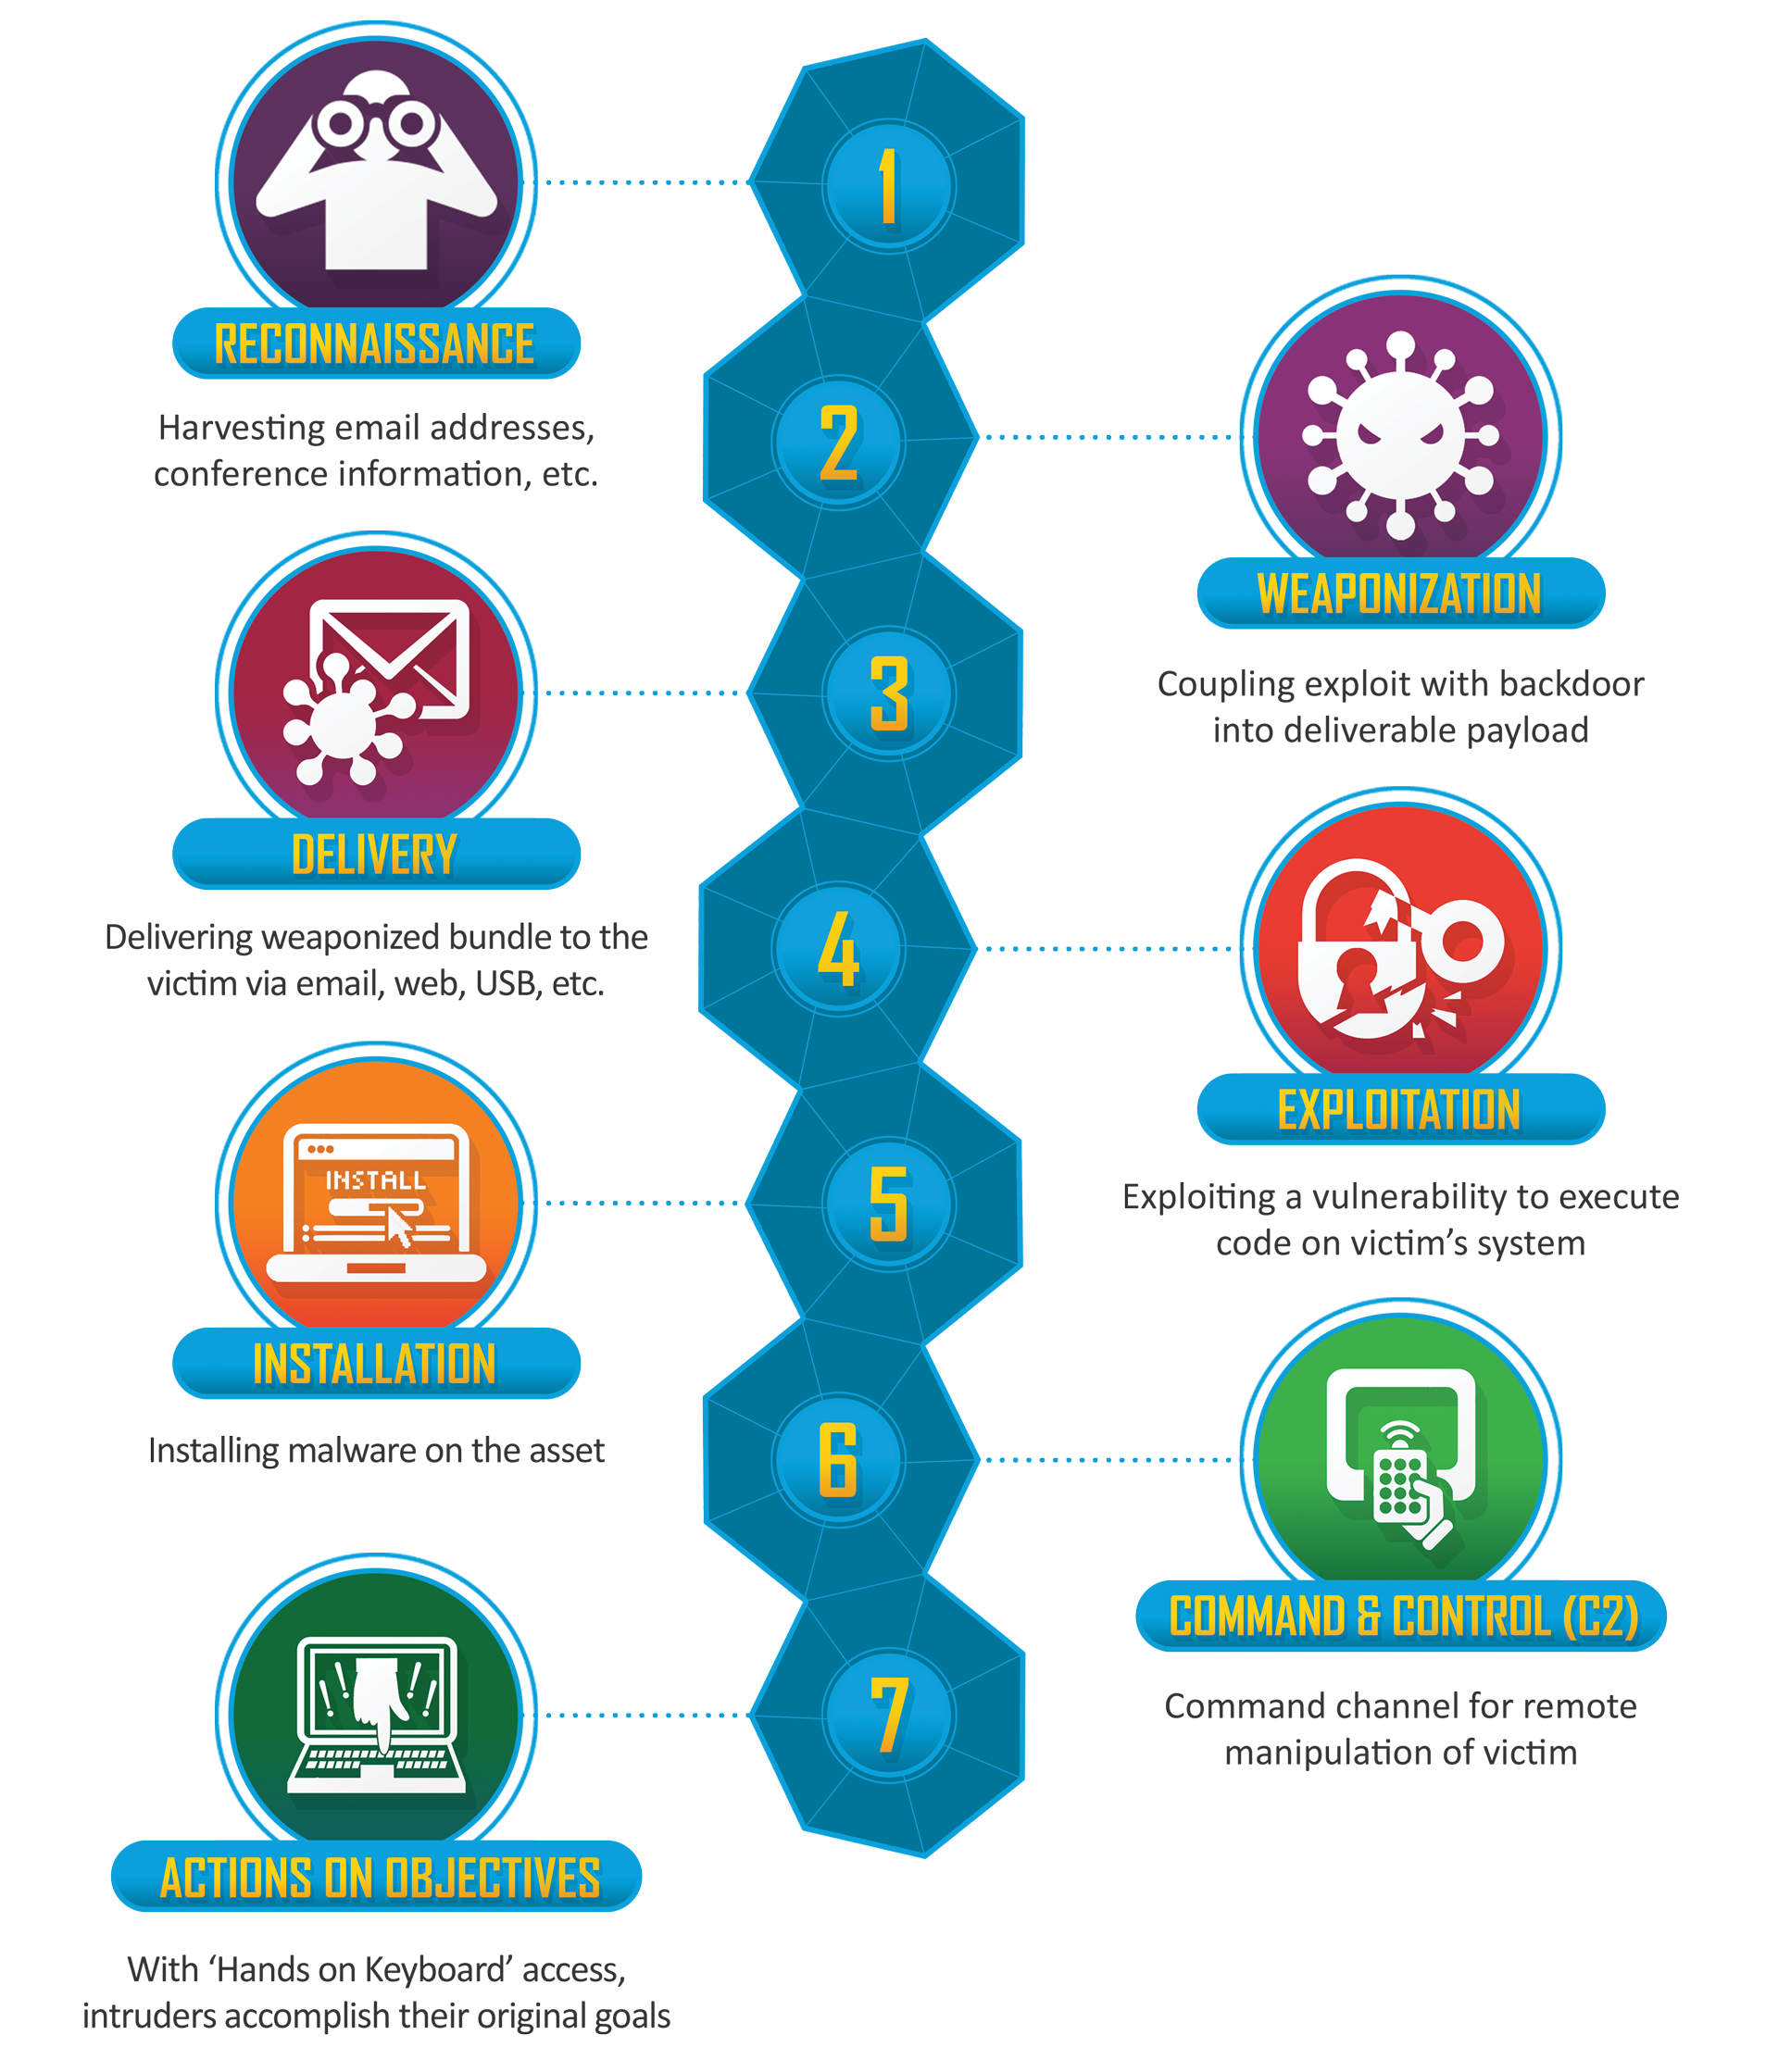
\includegraphics[width=0.7\textwidth]{cyber-kill-chain}
\caption{Schema che mostra i vari passi della Cyber Kill Chain.}
\end{figure}

%%
\section{Analisi dei malware}
L'analisi di un malware è un processo che consiste principalmente in due fasi: l'\textit{analisi statica} e l'\textit{analisi dinamica}. Con l'analisi statica si cerca di analizzare il malware senza eseguirlo, mentre con l'analisi dinamica lo si esegue per vederne il comportamento. Per capire cosa fa un malware spesso si ripete l'analisi più volte, sia statica che dinamica. I due tipi di analisi possono essere a loro volta suddivisi in \textit{analisi di base} e \textit{analisi avanzata}. Nelle analisi di base si va ad analizzare l'eseguibile senza addentrarsi nel codice in cui è stato scritto, mentre nelle analisi avanzate si eseguono operazioni come il reverse engineering o il debugging del codice malevolo. Per riepilogare i tipi di analisi da eseguire e che saranno illustrati nei prossimi capitoli sono:
\begin{enumerate}
\item Analisi statica di base
\item Analisi statica avanzata
\item Analisi dinamica di base
\item Analisi dinamica avanzata
\end{enumerate}

%%
\section{Comportamenti dei malware}
I malware sfruttano molte tecniche per cercare di mascherare il loro lavoro, non solo alla vittima ma anche ai malware analyst. Alcune di queste tecniche sono il cercare di capire se l'eseguibile sta girando su una macchina reale o su una macchina virtuale e per scoprirlo analizzano inanzitutto la quantità di risorse dedicate al sistema in termini di CPU, RAM e quantità di disco, inoltre analizzano i programmi installati sul dispositivo, per esempio, se sono presenti strumenti come Regshot oppure ProcessMonitor sanno che stanno girando sulla macchina di un malware analyst mentre se individuano programmi come Office oppure Adobe Reader sanno che la vittima è un normale utente. Tecniche più raffinate sono l'analizzare le date di creazione, di modifica e di accesso dei file, da cui si evince che, se sono troppo recenti, la macchina potrebbe essere stata appena creata con lo scopo di individuare e analizzare il malware in questione. 

Molti malware prima di connettersi alla rete, controllano se la connessione è disponibile. Il malware analyst può tentare di far credere al malware che la connessione sia disponibile utilizzando strumenti come FakeNet e InetSim.

%%
\section{Preparazione dell'ambiente}
Per eseguire l'analisi di un malware è importante preparare un ambiente in cui poterlo eseguire in modo sicuro, isolato e senza rischi per l'analizzatore.
Esistono i cosiddetti malware lab con macchine dedicate e con una rete completamente isolata, ma questo approccio è utilizzato da aziende e grandi organizzazioni.

Altrimenti, è possibile utilizzare delle macchine virtuali che hanno il vantaggio di isolare sia il sistema operativo sia la rete. Con le macchine virtuali si possono inoltre riportare a istantanee precedenti ed eliminare gli effetti di un malware.
La preparazione dell'ambiente virtuale procede come segue:
\subsection*{Scelta del software di virtualizzazione}
Scegliere il software che può fornirci la creazione di macchine virtuali. I software più famosi sono VMware, Hyper-V e VirtualBox. Il primo è un software commerciale e quindi a pagamento (ha una gestione migliore delle risorse per esperti), mentre gli altri due sono free. VirtualBox è quello che verrà utilizzato da qui in avanti all'interno di questo testo.
\subsection*{Creazione di una nuova macchina virtuale}
Per creare una macchina virtuale, in VirtualBox, basta cliccare su Nuova e impostare le caratteristiche che desideriamo, quali capacità del disco, memoria RAM dedicata, core del processore dedicati e stato della rete. In particolare è consigliato impostare come requisiti minimi le seguenti specifiche:
\begin{itemize}
\item Almeno 1 GB di memoria RAM;
\item Almeno 2 core del processore;
\end{itemize}
Meglio se le specifiche assegnati si avvicinano il più possibile a quelle di una macchina reale, poichè esistono delle categorie di malware che, per rendere più difficile il lavoro del malware analyst, cercano di capire se si trovano su macchine reali o virtuali e cambiare il loro comportamento.
\subsection*{Installazione del sistema operativo}
Prima di procedere all'installazione del sistema operativo sulla macchina, bisogna scaricare l'immagine ISO per l'installazione. Se si tratta di distribuzioni Linux o comunque sistemi open source, le immagini sono scaricabili gratuitamente, mentre per altri sistemi proprietari come Windows (il sistema che si userà in questo testo) è possibile reperire delle versioni per sviluppatore attive per un tempo limitato. \` Microsoft dà la possibilità di scaricare una macchina virtuale completa all'indirizzo: https://developer.microsoft.com/en-us/microsoft-edge/tools/vms.

Si può decidere se installare gli aggiornamenti o meno del sistema operativo; questo per fare in modo di avere una particolare vulnerabilità risolta  nel tempo da un particolare aggiornamento.

Su Windows bisogna disabilitare Windows Defender, sia in real time protection che in cloud protection. Questo perchè anche i tool utilizzati possono essere visti come malevoli.
\subsection*{Installazione dei software per l'analisi dei malware}
L'installazione degli strumenti per l'analisi dei malware può avvenire manualmente, installando i software desiderati. ecc.... su github script python che installa tutti i tool.
\subsection*{Configurazione della rete}
Configurare l'opzione di rete Host-Only (scheda solo host), per impedire al malware di diffondersi attraverso la rete e infettare dispositivi al di fuori della macchina virtuale. Con quest'opzione la rete sarà confinata solamente all'interno della macchina.
\subsection*{Creazione di un istantanea}
Prima di iniziare la prima analisi, è necessario catturare un'istantanea della macchina per poter ripristinare la macchina ad ogni nuova analisi.

%%
\section{Reperire i malware}
Per esercitarsi è possibile scaricare alcuni esempi di malware da diversi siti:
\begin{itemize}
\item Hybrid Analysis
\item ANY.RUN
\item VirusBay
\item VirusShare
\item VirusSign
\item https://zeltser.com/malware-sample-sources/
\end{itemize}

%%%%%%%%%%%%%%
%% analisi statica di base
\chapter{Analisi statica di base}
Nell'analisi statica di base il file malevolo viene analizzato senza essere eseguito. Si differenzia dall'analisi statica avanzata per il fatto che non si vanno a visualizzare le istruzioni del codice malevolo ma si visualizza solo la sua signature. In questo tipo di analisi si vanno, ad esempio, a verificare le stringhe presenti nel file PE. Viene utilizzata per capire la tipologia di file che stiamo analizzando, anche per evitare che alcuni malware si nascondano sotto altre tipologie di file.

Con l'analisi statica di base si va a vedere se un file è effettivamente un malware, se è impacchettato oppure no, quali librerie importa, quali servizi di sistema utilizza e se modifica o no chiavi di registro.

Il tipico processo svolto durante l'analisi statica di base è l'analisi delle stringhe.

%%
\section{Identificazione del file}
Determinare l'effettiva estensione del file è una delle parti principali di questa analisi. Gli hacker tentano infatti di dare una doppia estensione ai file per cercare di mascherare la vera estensione .exe facendo credere che siano ad esempio dei file PDF, documenti di testo o qualsiasi altra cosa appaia innocua.

Alcune volte gli attaccanti mascherano i malware da archivi autoestraenti: con un programma apposito (ad esempio con WinRar) creano un archivio che contiene il malware e scrivono uno script da eseguire all'apertura dell'archivio, in questo modo quando l'utente aprirà il file che sembrerà in tutto e per tutto un archivio compresso, lo script tirerà fuori il malware e lo eseguirà.

L'identificazione di un eseguibile di Windows avviene attraverso l'analisi della signature. In particolare un eseguibile di Windows avrà sempre i primi due bytes dedicati alle lettere \strings{MZ} in codifica ASCII, mentre un PDF inizierà sempre con \strings{\%PDF-}. Un archivio Zip inizia con i bytes dedicati alle lettere \strings{PK}. Questa caratteristica appartiene al DOS Header di ogni file PE, in particolare si tratta del campo e\_magic. Conoscendo questi particolari un programma, come quelli che saranno descritti in questo capitolo, possono facilmente identificare la tipologia di file.

\subsection*{\softwarename{File}}
da scrivere.

\subsection*{\softwarename{ExeInfo PE}}
da scrivere.

\subsection*{\softwarename{PEiD}}
PEiD è uno strumento simile a ExeInfo PE e da informazioni su un file PE analizzato. \\

Per prima cosa, aprire PEiD come amministratore e cliccare sul tasto "..." (tre puntini) per scegliere il file. Una volta scelto il file, la finestra principale di PEiD ci mostra alcune informazioni come... \\

La figura \ref{fig:peid-main} mostra l'analisi di un keylogger.

\begin{figure}[H]
\centering
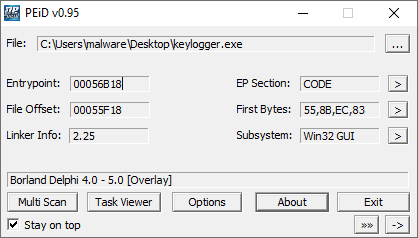
\includegraphics[width=0.65\textwidth]{peid-main}
\caption{Schermata iniziale di PEiD.}
\label{fig:peid-main}
\end{figure}


\subsubsection*{Plugin: Krypto ANALyzer}
Se si dispone del plugin Krypto ANALyzer (o KANAL) è possibile ottenere in una nuova finestra informazioni riguardanti vari algoritmi di codifica e cifratura utilizzati all'interno del malware. Un esempio è mostrato dalla figura \ref{fig:peid-kanal} che ci suggerisce l'utilizzo di ... per il keylogger analizzato sopra.

\begin{figure}[H]
\centering
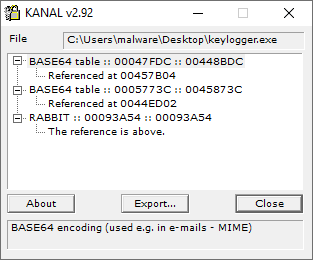
\includegraphics[width=0.50\textwidth]{peid-kanal}
\caption{Plugin KANAL di PEiD.}
\label{fig:peid-kanal}
\end{figure}

\subsection*{\softwarename{TriD}}
da scrivere. Utilizzando i pattern e non le signature non dice esattamente qual è la tipologia di file ma dà una probabilità sulla natura del file.

%%
\section{Calcolo dell'hash}
\`E possibile generare un hash del malware utilizzando diversi algoritmi come MD5, SHA-1, SHA-256, ecc.... Avere l'hash di un file malevolo è utile per farlo analizzare da servizi che cercano di individuarlo nei loro database. Il più famoso è VirusTotal: un servizio online che offre la possibilità di far analizzare un malware dai più conosciuti antivirus in commercio e fornisce i risultati delle analisi e le statistiche. Fornendo a VirusTotal l'hash del codice malevolo è in grado di dire se lo stesso file è già stato individuato in passato come sospetto. VirusTotal è disponibile all'indirizzo: https://virustotal.com.

...immagine virustotal

Alcuni strumenti utili per il calcolo dell'hash di un generico file sono descritti di seguito.

\subsection*{\softwarename{HashMyFiles}}
 
\subsection*{\softwarename{HashCalc}}

\subsection*{\softwarename{ComputeHash}}

%%
\section{Librerie e funzioni importate}
Durante l'analisi statica di base, è importante prestare molta attenzione alle llibrerie Windows, o DLL, importate dal malware. Le librerie più comunemente importate in un eseguibile Windows sono riassunte nella tabella sottostante:
\begin{table}[h!]
\centering
\begin{tabularx}{0.98\textwidth}{
	|  X 
	|  X
	|  X 
	| }
\hline
\textbf{Nome della libreria} & \textbf{Utilizzo da parte del sistema operativo} & \textbf{Utilizzo da parte dei malware} \\ [0.5ex]
\hline\hline
Kernel32.dll & utilizzata da tutti i programmi Windows & Permette al malware di interagire con il file system e la memoria RAM. \\
\hline
Advapi32.dll & manipolare i registri & Utilizzata dai malware per raggiungere persistenza.\\
\hline
User32.dll & gestire l'interfaccia utente & \\
\hline
Gdi32.dll & & \\
\hline
Ntdll.dll & & \\
\hline
WSock32.dll e Ws2\_32.dll & crea connessioni di rete & \\
\hline
Wininet.dll & implementare protocolli di rete HTTP/Https & \\
\hline
\end{tabularx}
\end{table}

Le funzioni più comunemente utilizzate dai malware dipendono dalle operazioni da eseguire.
\subsection*{Operazioni sulla memoria}
\subsubsection*{VirtualAlloc}
\subsubsection*{VirtualProtect}
\subsubsection*{VirtualFree}
\subsection*{Operazioni sui file}
\subsubsection*{CreateFile}
\subsubsection*{ReadFile}
\subsubsection*{WriteFile}
\subsubsection*{DeleteFile}
\subsection*{Operazioni sui registri}
\subsubsection*{RegCreateKey}
\subsubsection*{RegDeleteKey}
\subsubsection*{RegGetValue}
\subsubsection*{RegSetValueEx}
\subsubsection*{RegSetKeyValue}
\subsection*{Operazioni di rete}
connect, accept, send, recv, listen (utilizzata nei malware vettori), gethostbyaddr, gethostbyname,
InternetConnect
InternetReadFile
InternetWriteFile
\subsection*{Altre operazioni}
LoadLibrary
GetProcAddress
IsDebuggerPresent
WriteProcessMemory
CreateRemoteThread

altre: shellExecuteA significa che il malware lancia comandi
itoa: converte indirizzi ip in stringa (??)

%%
\section{Analisi delle stringhe} 
L'analisi delle stringhe consiste nel trovare le possibili stringhe presenti nell'eseguibile compilato e cercare di dare loro dei significati per comprendere se ci troviamo davanti ad un malware e quali sono le sue funzionalità.

Le stringhe che si vanno a cercare sono generalmente di due tipologie in base alla codifica: stringhe \textit{ASCII} o stringhe \textit{Unicode}. Nel caso delle stringhe ASCII ogni carattere della stringa viene codificato con un byte mentre nel caso dell'Unicode ogni carattere ha riservato 2 byte. In entrambe le codifiche ogni stringa viene terminata con il carattere nullo, rappresentato dallo 0.

esempio figura codifica

Gli hacker possono cercare di rendere difficile l'analisi delle stringhe tentando di impacchettare l'eseguibile. L'impacchettamento sarà descritto più avanti.

\subsection*{Stringhe di rete}
All'interno del malware possono trovarsi stringhe che in un certo qual modo indicano un'attività di rete da parte del malware. Queste stringhe possono essere indirizzi IP, nomi di host o indirizzi URL. Qui di seguiti sono indicati alcuni esempi di stringhe di rete:

...

\subsection*{Nomi di file}
Si possono trovare stringhe di nomi di file che possono riguardare file creati dal malware stesso oppure file che il malware va a ricercare all'interno del file system. Molto spesso si trovano stringhe con il nome stesso del malware e ciò indica che il malware tenta di creare copie di se stesso.

\subsection*{Stringhe di librerie}
Si può riconoscere una chiamata a librerie se sono presenti stringhe come: WriteFile, SetRegValue, ecc....

\subsection*{Stringhe di codifica}
La presenza di stringhe del tipo: "inserire stringa" indica l'utilizzo di codifica in Base64. La codifica in base64 infatti utilizza solo un determinato insieme di caratteri che comprende i numeri da 0 a 9, i caratteri da A a Z sia maiuscoli che minuscoli, il simbolo + e /. Una particolarità di questa codifica è che trasforma ogni tre byte in quattro e se la lunghezza finale non è divisibile per quattro si aggiungono i simboli di uguale =.

Per capire quindi se la codifica in base64 è stata utilizzata, dovremmo trovare la stringa A---z0---9+/ oppure stringhe che finiscono con uno o più simboli di uguale.

\subsubsection*{XORSearch}


\subsection*{Chiavi di registro}
Chiavi di registro come stringhe indicano che il malware accede, modifica, crea o cancella chiavi di registro. Ciò viene fatto di solito quando l'eseguibile malevolo vuole raggiungere una certa persistenza sulla macchina.

\subsection*{Altre stringhe}
Altre stringhe che si possono trovare sono stringhe che indicano funzionalità del malware come:

...

\subsection*{Strings}

%%
\section{Data di compilazione}
Coloro che scrivono malware tendono spesso a nascondere la vera data di compilazione che può risultare molto indietro nel tempo oppure addirittura nel futuro. \`E molto utile associare la data di compilazione con altre date all'interno dell'eseguibile come i timestamp associati alle risorse: una grossa differenza in termini di anni può indicare una manomissione della data di compilazione e far crescere il sospetto che il file analizzato sia un file malevolo.

%%
\section{Strumenti per l'analisi statica di base}
L'intera analisi statica di base si basa essenzialmente sull'analisi dei cosiddetti file PE di Windows. Il PE file (si veda l'Appendice A per saperne di più sui PE file) ci può dare molte informazioni sulle librerie importate, lo spazio di memoria allocato per l'eseguibile e molto altro. 

Prima di analizzare come è composto un PE file è importante capire che l'importazione delle librerie utilizzate da un eseguibile può avvenire in tre modi:
\begin{itemize}
\item Statica: tipica dei sistemi Unix, quando si compila un file, le librerie richiamate dal file stesso vengono incluse nell'eseguibile e non è quindi necessario risolvere nessun riferimento.
\item Dinamica: le librerie utilizzate dal file vengono caricate in memoria nel momento in cui l'eseguibile viene caricato in memoria. I nomi e i riferimenti delle librerie da caricare vengono forniti dal campo Import Address Table.
\item Runtime: viene utilizzata principalmente da chi scrive malware. Le librerie vengono caricate nello spazio di memoria allocato dall'esecuzione del malware nel momento in cui vengono chiamate dal malware stesso. Le librerie \textbf{LoadLibrary} e \textbf{GetProcAddress} vengono spesso utilizzate per caricare altre librerie, ed è un forte indicatore del fatto che il malware è stato impacchettato.
\end{itemize}

Ogni file PE è composto da diversi header tra cui DOS Header, PE Header, File Header e Optional Header che sono essenzialmente delle strutture con all'interno diversi campi utili a identificare meglio l'eseguibile analizzato. In particolare, all'interno dell'Optional Header, il campo Magic ci dice se il file è un eseguibile per architetture a 32 bit o a 64 bit, il campo AddressOfEntryPoint indica il puntatore da cui iniziare ad eseguire il codice. I malware possono però effettuare altri controlli prima di questo puntatore quindi non sempre è realmente indicativo dell'inizio delle istruzioni eseguibili. Un altro campo DataDirectory, che contiene il riferimento a diverse tabelle tra cui:
\begin{itemize}
\item Tabella Export Directory: importante se il file eseguibile è una libreria, cioè un DLL. Le funzioni in questa tabella vengono rese disponibile esternamente a chi esegue la libreria.
\item Tabella Import Directory: specifica tutte le librerie importate dal malware. Le librerie da importare sono specificate nel Import Address Table e l'importazione avviene con riferimento dinamico.
\item Tabella Resource Directory: contiene le risorse utilizzate dal file, come le icone.
\item Import Address Table: specifica tutte le librerie che il malware deve importare in memoria. Si tratta di una lista di funzioni per ogni file DLL specificato. Ci possono essere due modi per caricare le librerie contenute nella tabella: il primo consiste da parte del loader nel sostituire il nome contenuto nella tabella con l'effettivo indirizzo della libreria per indicare al malware dove recuperarle; il secondo metodo consiste nel utililzzare un valore ordinale delle funzioni all'interno di una DLL al posto del nome delle funzioni. figura...
\end{itemize}

Un indicatore che ci suggerisce che ci troviamo di fronte ad un malware impacchettato è la presenza di sezioni con nomi diversi da quelli tipici di un PE file e con permessi sia di esecuzione che di scrittura.

Per analizzare un file PE, e completare tutte i tipi di analisi descritti in questo capitolo, si possono utilizzare gli strumenti descritti qui di seguito.

I malware utilizzano le risorse per immagazzinare codice malevolo o file di configurazione. I trojan, che si mascherano da programmi legittimi, nascondono ad esempio dei file PDF malevoli all'interno delle risorse che verranno eseguiti una volta lanciato il trojan.

\subsection*{\softwarename{PEStudio}}
\`E un software pensato appositamente per fare malware analysis, infatti PEStudio tenta già di dare delle indicazioni sui campi analizzati per dire se sono malevoli o no. \`E possibile scaricare una versione PEStudio dal sito "https://www.winitor.com/features" dove sono disponibili sia una versione gratuita che a pagamento.\\

Innanzitutto avviare PEStudio come amministratore, dopodichè importare in PEStudio il file che si vuole analizzare trascinandolo sulla finestra del programma oppure cliccando su \softwarecommand{file > open file} e selezionando dalle cartelle il file da analizzare.\\

Possiamo guardare il contenuto del file header cliccando sulla sezione a sinistra \softwarecommand{file header}. Guardando l'esempio in figura \ref{fig:pestudio-fileheader} notiamo informazioni come la data di compilazione in cui una data di compilazione molto vecchia (in questo caso 2014) potrebbe essere un tentativo di depistaggio da parte dell'attaccante per nascondere il malware. Altre informazioni utili sono \softwarecommand{machine} che indica l'architettura del file (in questo caso x86), il numero di sezioni viene dato da \softwarecommand{section}. Tutte le restanti informazioni riguardano il campo delle caratteristiche.\\

\begin{figure}[H]
\centering
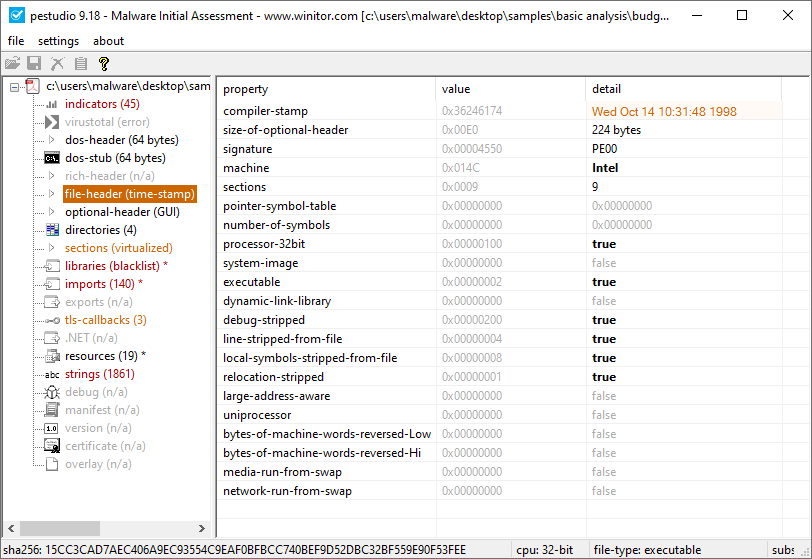
\includegraphics[width=0.65\textwidth]{pestudio-fileheader}
\caption{Schermata che mostra le informazioni estrapolate dal File Header del file caricato in PEStudio.}
\label{fig:pestudio-fileheader}
\end{figure}

Cliccando invece su \softwarecommand{optional header} si possono vedere le informazioni riguardanti l'Optional Header del file PE. La figura \ref{fig:pestudio-optionalheader} mostra il campo magic che contiene PE, l'entry point che ci indica il punto della memoria dove iniziare ad eseguire il codice (in questo caso section:.text indica che il codice parte dalla sezione .text), la dimensione del codice è indicata dal campo size-of-code e l'image base, indicato da image-base indica il punto di caricamento del PE file per il Loader.\\

\begin{figure}[H]
\centering
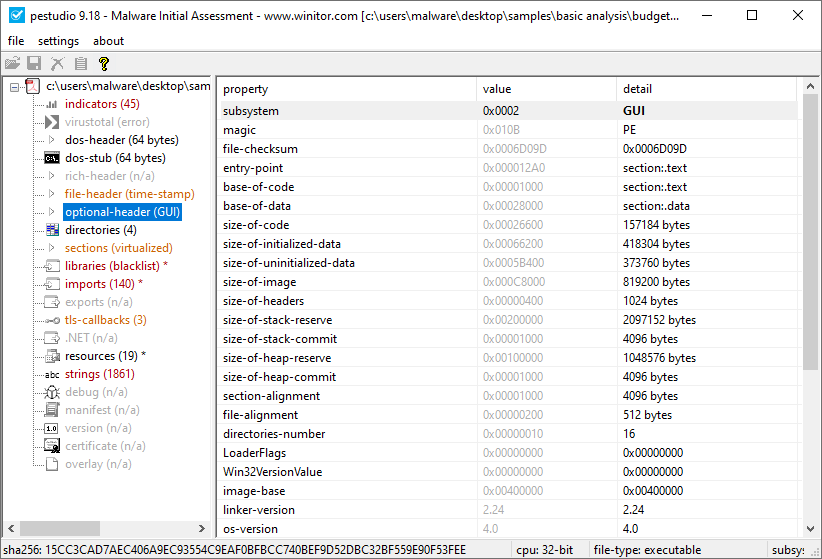
\includegraphics[width=0.65\textwidth]{pestudio-optionalheader}
\caption{Schermata che mostra le informazioni contenute nell'Optional Header del file PE caricato in PEStudio.}
\label{fig:pestudio-optionalheader}
\end{figure}

Una funzionalità importante è la visualizzazione delle sezioni che è possibile cliccando su \softwarecommand{sections} alla sinistra del programma come mostrato dalla figura \ref{fig:pestudio-sections}. Qui è importante guardare se sono presenti sezioni con nomi inusuali e che hanno permessi sia di esecuzione che di scrittura. Il campo name ci indica il nome della sezione e i campi executable, readable e writeable i vari permessi.\\

\begin{figure}[H]
\centering
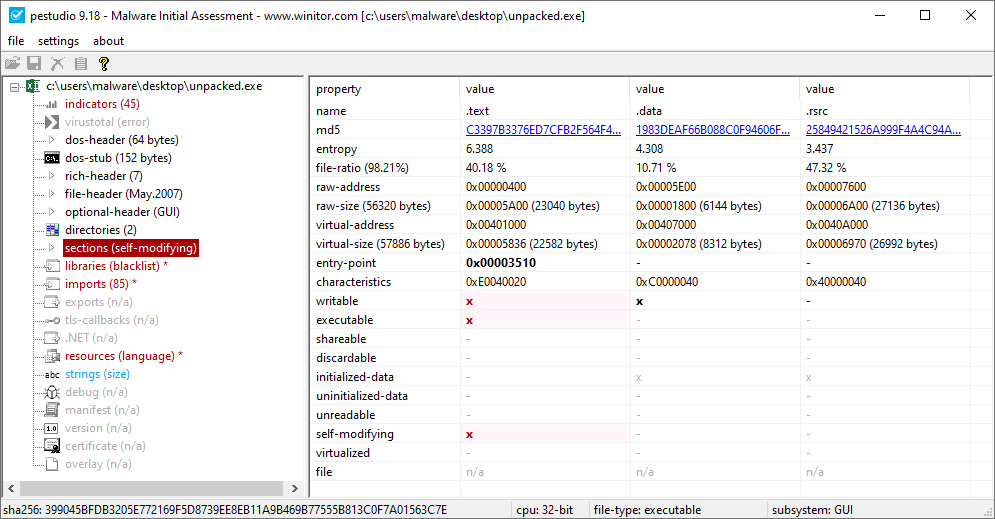
\includegraphics[width=0.65\textwidth]{pestudio-upxunpacked-sections}
\caption{Informazioni riguardanti le sezioni di un file PE in PEStudio.}
\label{fig:pestudio-sections}
\end{figure}

La sezione \softwarecommand{libraries} ci mostra le librerie importate dal PE file malevolo. Nel malware analizzato in figura \ref{fig:pestudio-libraries} notiamo che il file PE importa librerie come \strings{wininet.dll} e \strings{ws2\_32.dll} che indicano un'attività di rete da parte del malware e sono state riconosciute da PEStudio come sospette e quindi segnate da una X in rosso. \\

\begin{figure}[H]
\centering
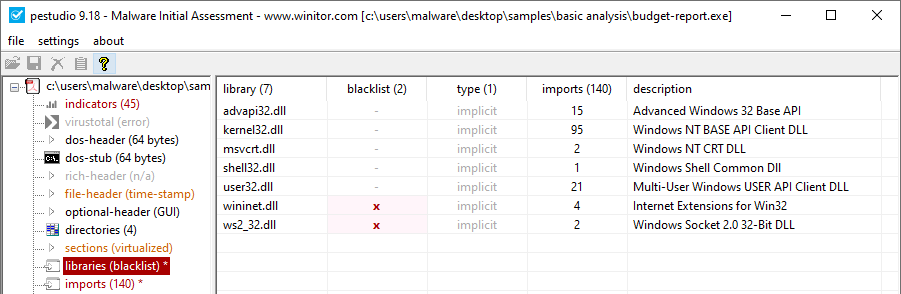
\includegraphics[width=0.65\textwidth]{pestudio-libraries}
\caption{Analisi delle librerie contenute in un file PE attraverso PEStudio}
\label{fig:pestudio-libraries}
\end{figure}

La sezione \softwarecommand{imports} mostra tutte le funzioni importate dal PE file. Anche in questo caso PEStudio ci segna quelle potenzialmente sospette. Dalla figura \ref{fig:pestudio-imports} possiamo notare comunque la presenza di librerie che possono indicare un'azione malevola da parte dell'eseguibile, in particolare: 
... elenco librerie\\

\begin{figure}[H]
\centering
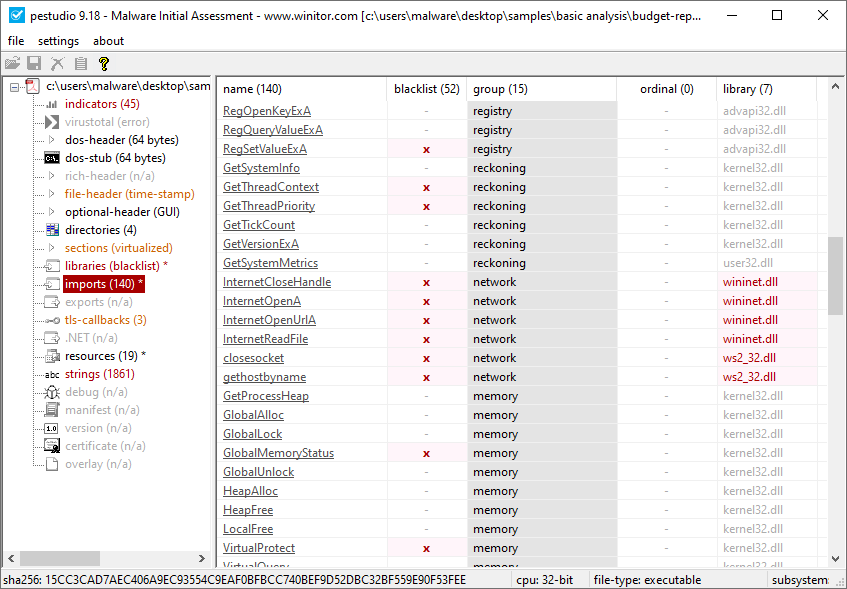
\includegraphics[width=0.65\textwidth]{pestudio-imports}
\caption{Analisi delle librerie importate all'interno di un file PE attraverso PEStudio.}
\label{fig:pestudio-imports}
\end{figure}

Nel campo risorse PE Studio ci fornisce la tipologia del contenuto della risorsa, la signature, la lingua che di solito viene specificata dal programmatore del malware oppure viene impostata in automatico dal compilatore del malware. Nelle risorse di un file PE, un attaccante può includere una risorsa di tipo eseguibile che spesso può essere il vero malware nascosto come in figura \ref{fig:pestudio-resources}. \\

\begin{figure}[H]
\centering
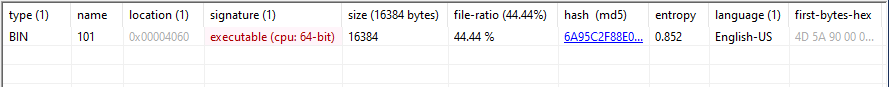
\includegraphics[width=0.85\textwidth]{pestudio-resources-exec}
\caption{Esempio di risorsa malevola contenuta in un file PE analizzata con PEStudio. In questo caso si può notare che come risorsa è stato inserito un eseguibile.}
\label{fig:pestudio-resources}
\end{figure}

Molto importante è la sezione \softwarecommand{strings} che ci mostra le stringhe trovate dall'analisi del file PE. La figura\ref{fig:pestudio-strings} mostra le come vengono rappresentate le stringhe e come PEStudio suggerisce già i possibili utilizzi delle stringhe. Analizzando con PEStudio un esempio di keylogger potremmo trovare all'interno le seguenti stringhe:

... elenco stringhe
... descrizione delle stringhe.\\

\begin{figure}[H]
\centering
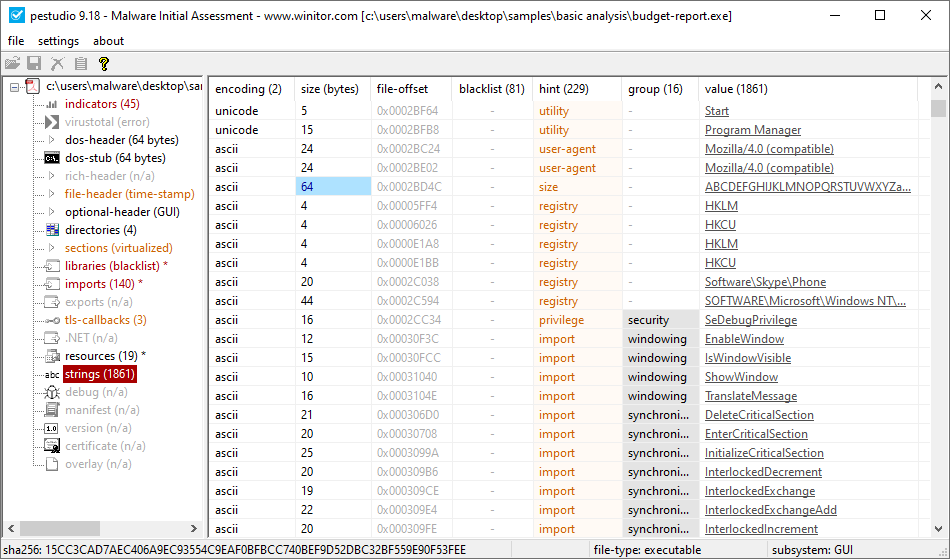
\includegraphics[width=0.65\textwidth]{pestudio-strings}
\caption{Elenco delle stringhe trovate all'interno di un file PE con l'analisi delle stringhe in PEStudio.}
\label{fig:pestudio-strings}
\end{figure}

La funzione \strings{Sleep} è spesso un segnale d'allarme poichè viene utilizzata dai malware per aggirare software antivirus o anti-malware.

Altre sezioni meno importanti per l'analisi sono \softwarecommand{directories}, che indica le data directories.

Un problema che può sorgere nell'analisi di un malware è il fatto che il malware può essere impacchettato. Per analizzare un malware impacchettato bisogna prima spacchettarlo. Per fare ciò si rimanda al capitolo sull'offuscamento.

\subsection*{\softwarename{PEView}}
Un altro software per l'analisi di un file PE è PEView. A differenza di PEStudio ...\\

Per analizzare un file con PEView la prima cosa da fare è avviare il programma con i privilegi di amministratore e verrà subito chiesto di selezionare dalle cartelle il file malevolo da visualizzare. Una volta fatto ciò PEView mostra i dati contenuti nel file PE come in figura \ref{fig:peview-main}. \\

\begin{figure}[H]
\centering
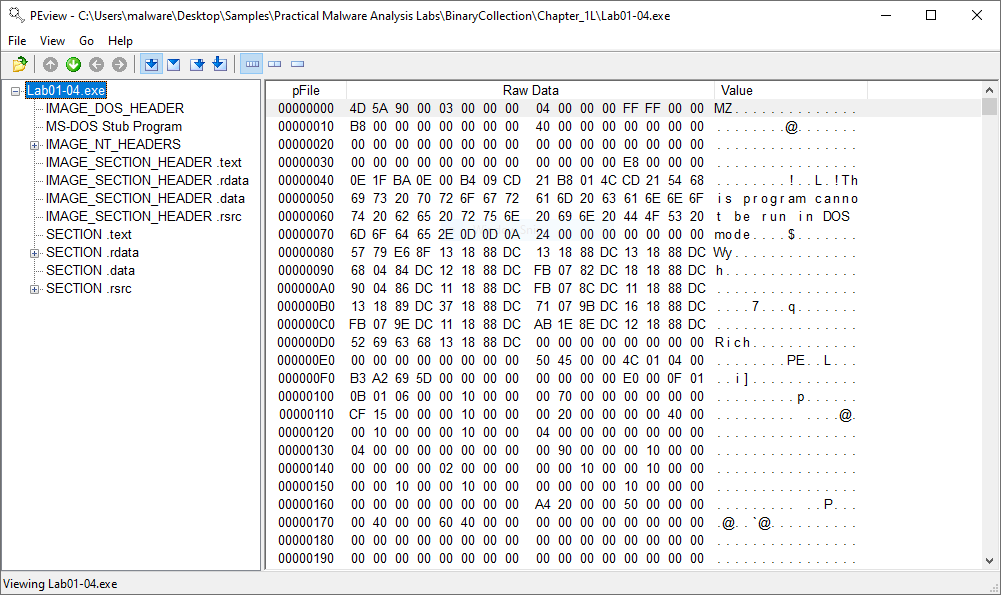
\includegraphics[width=0.65\textwidth]{peview-main}
\caption{Schermata iniziale mostrata da PEView al caricamento di un file.}
\label{fig:peview-main}
\end{figure}

Nella parte sinistra della finestra di PEView è possibile vedere anche il contenuto delle sezioni dell'eseguibile e dei vari header. Spesso all'interno dei malware viene inserito del codice eseguibile all'interno della sezione dedicata alle risorse; con PEView è possibile identificare eventuali risorse eseguibili. Nella figura \ref{fig:peview-addresstable} è possibile vedere il contenuto dell'import address table.\\

\begin{figure}[H]
\centering
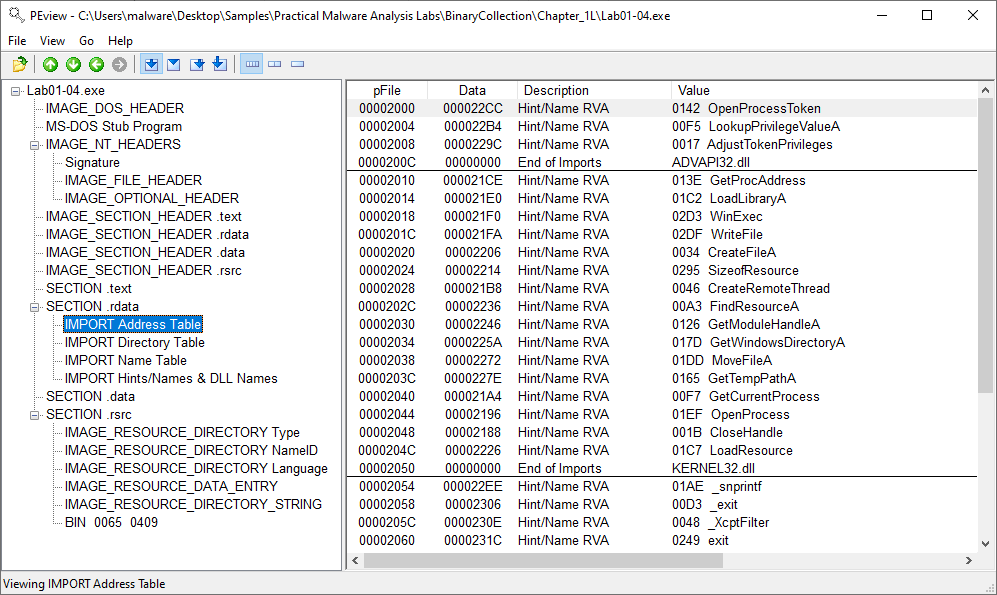
\includegraphics[width=0.65\textwidth]{peview-addresstable}
\caption{Sezione di un file PE contenente la Import Address Table visualizzata con PEView.}
\label{fig:peview-addresstable}
\end{figure}

\subsection*{\softwarename{CFF Explorer}}
Consente anche di modificare eventualmente i campi del PE file.

%%%%%%%%%%%%%%
%% analisi dinamica di base
\chapter{Analisi dinamica di base}
L'analisi dinamica è quel tipo di analisi in cui si esegue il malware e si valutano le modifiche effettuate sul sistema operativo. L'esecuzione di un malware può portare a modifiche del sistema come la creazione, l'eliminazione o la modifica dei registri di Windows, può generare traffico di rete nel momento in cui si collega a server remoti e scarica altri file sul sistema, può lanciare ulteriori processi e fare in modo di avviarsi in automatico oppure modificare a proprio piacimento il file system della vittima.

Per comprendere meglio questo tipo di analisi sui sistemi Windows si consiglia la lettura dell'appendice sul sistema Windows, in particolare sulle Windows API e sul registro di sistema.

\section{Modifica del file system}
I malware agiscono sul file system creando, eliminando o modificando file. Le funzioni interessate sono \strings{CreateFile}, \strings{ReadFile} e \strings{WriteFile}. Se, tramite analisi statica, notiamo che un malware importa queste funzioni significa che ha capacità di creare, leggere e scrivere file.

Altre funzioni potenzialmente utilizzate da un malware sono \strings{CreateFileMapping} e \strings{MapViewOfFile}. Vengono usate per emulare il comportamento del Windows Loader, cioè il processo che si occupa di caricare un file in memoria, per caricare in autonomia dell'altro codice malevolo in memoria.

\section{Modifica dei registri}
Tipicamente l'accesso ai registri non prevede l'utilizzo dei privilegi di amministratore. I malware utilizzano particolari chiavi per raggiungere determinati scopi.

Le funzioni tipicamente utilizzate per modificare i registri sono: \strings{RegOpenKeyEx}, \strings{RegSetValueEx} e \strings{RegGetValue}. Un malware che importa queste funzioni ha la capacità di leggere e impostare nuove chiavi di registro e valori associati alle chiavi.

\subsection*{Creare persistenza}
La cartella di registro \strings{HKLM\textbackslash{}SOFTWARE\textbackslash{}Microsoft\textbackslash{}Windows\textbackslash{}CurrentVersion\textbackslash{}Run} stabilisce quali programmi vengono lanciati nel momento in cui un utente effettua l'accesso alla macchina. Un malware può modificare questa cartella e aggiungere una chiave con il proprio nome e un valore con il percorso del file da eseguire all'avvio per assicurarsi di essere eseguito ogni volta che l'utente accede al proprio account. In questo modo si dice che il malware ha \textit{raggiunto persistenza}.

Altre cartelle di registro simili utilizzate per creare persistenza sono:
\begin{itemize}
\item \strings{HKLM\textbackslash{}SOFTWARE\textbackslash{}Microsoft\textbackslash{}Windows\textbackslash{}CurrentVersion\textbackslash{}RunOnce}
\item \strings{HKLM\textbackslash{}SOFTWARE\textbackslash{}Microsoft\textbackslash{}Windows\textbackslash{}CurrentVersion\textbackslash{}RunServices}
\item \strings{HKLM\textbackslash{}SOFTWARE\textbackslash{}Microsoft\textbackslash{}Windows\textbackslash{}CurrentVersion\textbackslash{}RunServicesOnce}
\item \strings{HKLM\textbackslash{}SOFTWARE\textbackslash{}Microsoft\textbackslash{}Windows\textbackslash{}CurrentVersion\textbackslash{}Policies\textbackslash{}Explorer\textbackslash{}Run}
\item \strings{HKLM\textbackslash{}SOFTWARE\textbackslash{}Microsoft\textbackslash{}Windows\textbackslash{}CurrentVersion\textbackslash{}Windows\textbackslash{}AppInit\_DLLs}
\end{itemize}

... spiegazione + controllare che HKLM sia giusto.

\subsubsection*{\softwarename{Autoruns}}
Autoruns è un semplice software interno di Windows che mostra tutti i possibili modi in cui un malware può raggiungere persistenza sulla macchina. Questo strumento si occupa di scansionare tutti i registri e tutto ciò che un malware può cambiare per auto avviarsi e lo mostra all'utente per ogni cartella di registro citata precedentemente.

Autoruns cerca di evidenziare in rosso i programmi che non hanno una firma valida, ma bisogna fare attenzione perchè possono essere evidenziati anche programmi legittimi che però non sono verificati.

\section{Attività di rete del malware}
Un malware, durante la sua esecuzione, può generare traffico di rete e connettersi a server remoti oppure fare esso stesso da server e accettare connessioni in entrata. Può quindi avere un ruolo da client o da server ed è importante capire il suo funzionamento, e per farlo si può analizzare l'ordine di chiamata delle funzioni della libreria di Windows \strings{Ws2\_32.dll}.

Nel caso in cui il malware si comporti come un \textbf{server} il suo scopo sarà quello di mantenere attiva una socket in ascolto per le connessioni in arrivo da remoto, quindi, a livello di programmazione le funzioni saranno chiamate nell'ordine:
\begin{enumerate}
\item \strings{socket}
\item \strings{bind}
\item \strings{listen}
\item \strings{accept}
\item \strings{send} e \strings{recv}
\end{enumerate}

Inanzitutto il malware chiama la funzione WSAStartup(), dopodichè crea una socket (funzione \strings{socket}) e la collega ad una porta con \strings{bind} e la mette in ascolto delle connessioni (funzione \strings{listen}). All'arrivo di una richiesta di connessione remota, utilizza la funzione \strings{accept} per accettarla e successivamente inviare oppure ricevere dati (\strings{send} e \strings{recv}).\\

Nel caso invece in cui il malware si comporti come un \textbf{client} il suo scopo sarà quello di connettersi ad un socket remoto ed inviare dati personali della vittima oppure scaricare dati come un ulteriore codice malevolo da eseguire. In questo caso l'ordine di chiamate delle funzioni della libreria \strings{Ws2\_32.dll} è il seguente:
\begin{enumerate}
\item \strings{socket}
\item \strings{connect}
\item \strings{send} e \strings{recv}
\end{enumerate}

Per prima cosa il malware utilizza la funzione \strings{socket} per creare una socket e successivamente la funzione \strings{connect} per connettersi, tramite la socket appena creata, al server remoto. Una volta stabilita la connessione invia e riceve dati a proprio piacimento (funzioni \strings{send} e \strings{recv}).\\

Analizzare il traffico con strumenti di sniffing è una tecnica di analisi molto importante
risoluzione di nomi dns inusuali vengono usati per scaricare dati dai malware.
Utilizzo del protocollo HTTP GET request utilizzate in due modi: scaricare malware sulla macchina della vittima, raccogliere informazioni utili per contattare il server Command and Control.
Le richieste POST sono utilizzate per salvare dati copiati sulla macchina della vittima (es. password). Dalle richieste POST è possibile recuperare i dati del pacchetto.
Anche il protocollo FTP può essere utilizzato. Ultimamente vengono usati anche protocolli per Samba o protocolli per il servizio email.

\subsection*{\softwarename{Wireshark}}
Wireshark è uno dei più conosciuti software per effettuare lo sniffing di pacchetti di rete ed analizzare così il traffico di una rete. In questo contesto è molto utile per capire quali operazioni un malware compie attraverso internet e come cerca di comunicare con altri dispositivi in rete.

All'apertura di Wireshark come amministratore viene chiesto di scegliere quale interfaccia di rete monitorare; una volta scelta si vedrà subito attiva la cattura di tutti i pacchetti che viaggiano in rete in una schermata simile a quella in figura \ref{fig:wireshark-main}.

\begin{figure}[H]
\centering
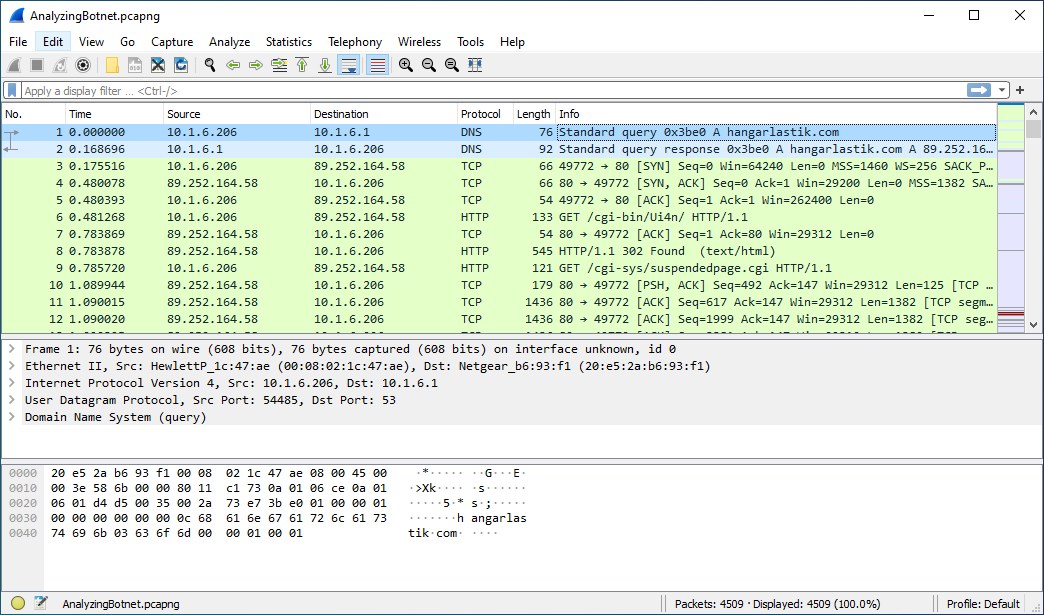
\includegraphics[width=0.98\textwidth]{wireshark-main}
\caption{Schermata principale di Wireshark e cattura di alcuni pacchetti che viaggiano attraverso la rete.}
\label{fig:wireshark-main}
\end{figure}

La finestra principale di Wireshark è suddivisa in tre schede: \textit{Packet List}, \textit{Packet Details} e \textit{PacketBytes}.

La prima scheda in alto (\textit{PacketList}) mostra essenzialmente la lista dei pacchetti catturati e alcuni campi con le informazioni essenziali. Questi campi sono:
\begin{itemize}
\item \softwarecommand{No.}: indica il numero in ordine del pacchetto;
\item \softwarecommand{Time}: tempo espresso in millisecondi che indica l'arrivo di un pacchetto;
\item \softwarecommand{Source}: l'indirizzo IP sorgente del pacchetto;
\item \softwarecommand{Destination}: l'indirizzo IP di destinazione del pacchetto;
\item \softwarecommand{Protocol}: il protocollo dello stack TCP/IP a cui appartiene il pacchetto;
\item \softwarecommand{Length}: la lunghezza in byte del pacchetto;
\item \softwarecommand{Info}: informazioni sommarie sul pacchetto selezionato;
\end{itemize}

\`E inoltre possibile aggiungere ulteriori campi come le porte sorgente e destinazione di un pacchetto. Per farlo basta cliccare con il tasto destro su una colonna a caso e cliccare su \softwarecommand{Column Preferences...}, si aprirà una finestra popup dove si può aggiungere una nuova colonna con il tasto \softwarecommand{+} nella sezione \softwarecommand{Appearance} > \softwarecommand{Columns}. Se si vogliono aggiungere i campi per la porta sorgente e destinazione nei valori delle nuove colonne si deve impostare rispettivamente \textit{Src port (unresolved)} e \textit{Dest port (unresolved)}.\\

La seconda scheda nel mezzo è la scheda \textit{Packet Details} e mostra proprio i dettagli degli header per ogni pacchetto che si seleziona. Gli header vengono suddivisi per livelli dello stack TCP/IP e ogni livello mostra i valori di ogni campo. Si possono creare nuove colonne nella lista dei pacchetti della scheda precedente con il valore di un particolare campo cliccando con il tasto destro sul campo e cliccando \softwarecommand{Apply as Column}.\\ 

L'ultima scheda, \textit{PacketBytes}, che si trova nella parte inferiore in figura \ref{fig:wireshark-main} mostra sulla sinistra il valore in byte del contenuto dell'intero pacchetto e ne fornisce, sulla destra, una possibile decodifica in un linguaggio umano. Selezionando con il mouse i campi degli header nella scheda \textit{Packet Details} è possibile vedere in modo automatico la corrispondente selezione in byte di quei campi.

\subsubsection*{Impostare dei filtri}
Su Wireshark è possibile impostare dei filtri per mostrare solo i pacchetti di reale interesse senza tenere conto di tutti gli altri pacchetti del traffico di rete.\\
\shellcommand{http.request or ssl.handshake.type == 1}
serve a mostrare solo i pacchetti di tipo HTTP o SSL/TLS.

Se si vogliono filtrare pacchetti per indirizzi IP sorgente e/o destinazione si possono scrivere filtri come\\
\shellcommand{ip.src == 192.168.1.1\\ip.dst == 151.183.38.3\\ip.addr == 192.168.1.2}

Se invece si vogliono filtrare solamente pacchetti HTTP (sia richieste che risposte) si può scrivere il filtro\\
\shellcommand{http.request or http.response}

Nel caso in cui si voglia filtrare solo uno o più pacchetti che contengono una determinata stringa (può essere ad esempio il nome o il percorso di una risorsa di un pacchetto HTTP GET) si può inserire filtri del tipo\\
\shellcommand{frame contains stringa}
e si otterranno tutti i pacchetti in cui c'è la stringa \textit{''stringa''}.

\subsubsection*{Salvare una configurazione}
Per salvare una configurazione andare su \softwarecommand{Edit} > \softwarecommand{Configuration Profiles...} e una volta aperta la finestra di configurazione cliccare sul tasto \softwarecommand{+} e assegnare un nuovo nome.

\subsubsection*{Seguire un flusso TCP}
Su Wireshark possiamo selezionare un pacchetto TCP o di livello applicativo e con il tasto destro cliccare \softwarecommand{Follow} > \softwarecommand{TCP Stream}. Questa funzione è molto utile poichè permette di mostrare in una sola finestra l'intero scambio di pacchetti in quella connessione TCP, riuscendo anche a mostrare i dati inviati tramite eventuali richieste POST o GET. (è giusto?)

\section{Esecuzione di ulteriore codice}
Eseguendo un malware è interessante analizzare i metodi in cui un malware esegue ulteriore codice generato dal malware stesso, oppure scaricato da un server malevolo. Ci sono principalmente quattro modi: tramite \textit{DLL}, con \textit{processi}, utilizzando \textit{thread} o utilizzando \textit{servizi}.\\

Le DLL sono utilizzate da un malware per caricare codice malevolo contenuto all'interno del DLL.
I malware possono anche dirottare il caricamento di DLL fruttando il loro ordine di ricerca da parte dell'eseguibile che deve caricarne le librerie. Si può immaginare uno scenario in cui un programma eseguibile, tale \strings{programma.exe}, ha bisogno dei riferimenti alle librerie utilizzate all'interno del proprio codice ed inizia a cercare il proprio DLL, detto \strings{esempio.dll}, per prima cosa all'interno della cartella dove è contenuto il programma. All'interno della cartella però non è presente il file ed allora lo si cerca in windows/system32 ma non è presente nemmeno lì, allora si va a cercarla in windows, poi nella cartella corrente ed infine, se non è presente nemmeno nella cartella corrente si va in \strings{\%PATH\%}. Un malware che vuole cercare di far eseguire a \strings{programma.exe} una copia malevola di \strings{esempio.dll} al posto di quella autentica sfrutta questo ordine di ricerca stabilito dal sistema inserendo la propria copia nella cartella del programma: in questo modo, supponendo che \strings{esempio.dll} autentico sia presente in \strings{\%PATH\%}, il sistema si interromperà subito avendo trovato un file con lo stesso nome all'inizio della sua ricerca. Verrà quindi eseguita la copia malevola di \strings{esempio.dll} al posto di quella originale.\\

L'esecuzione di codice tramite processi permette al malware di lanciare un eseguibile con proprie risorse e thread. Viene sfruttata la funzione \strings{CreateProcess} con il passaggio del parametro \strings{STARTUPINFO} che contiene la gestione dello standard input, dello standard output e dello standard error. Un malware può creare una socket per connettersi ad una shell remota e ...?\\

L'esecuzione tramite Thread, ovvero i vari pezzi di un processo, permette al malware di avere uno spazio di memoria per permettere l'esecuzione parallela dei thread ed ogni thread ha la propria stack e registri. Il malware utilizza createThread con parametro start che indica l'indirizzo di una funzione per dare a start un istruzione malevola. Il malware può comunicare con il server di Command And Control senza lanciare un'applicazione e quindi senza che sia rilevabile in modo evidente dal sistema operativo.\\

I servizi sono le applicazioni che vengono eseguite in background dal sistema operativo senza l'input di un utente. I malware usano due tipologie di servizi per raggiungere persistenza: servizi WIN32\_SHARE\_PROCESS (svchost.exe) e servizi WIN32\_OWN\_PROCESS. I servizi implementati si possono trovare nel registro di sistema \strings{HKLM\textbackslash{}System\textbackslash{}CurrentControlSet\textbackslash{}Services} dove un valore di Start uguale a 0x03 sta per ''Load on Demand'' e un valore di Type uguale a 0x20 sta per ''WIN32\_SHARE\_PROCESS''. Per sapere se un malware vuole raggiungere persistenza si devono ricercare le librerie:
OpenSCManager
CreateService
StartService

\section{System Integrity Monitoring}
\`E una tecnica per effettuare l'analisi dinamica di base e consiste nel catturare un istantanea del file system prima di eseguire il malware, una dopo l'esecuzione del malware e confrontarle per capire quali modifiche sono state apportate al sistema. Tipicamente si attende qualche minuto prima di eseguire la seconda istantanea in modo da dare al malware il tempo di compiere tutte le operazioni per il quale è stato programmato.

Con questa tecnica si possono identificare eventuali cambiamenti apportati a file come modifiche, creazioni, eliminazioni e cambiamenti apportati alle chiavi di registro.

Questa tecnica ha però delle limitazioni; non si possono conoscere eventuali modifiche riguardanti il kernel, quindi i malware di tipo rootkit non sono rilevabili, inoltre non sempre si riesce a tenere traccia dei file temporanei creati durante l'esecuzione malevola. \`E importante sapere che non tutti i cambiamenti rilevabili nella seconda istantanea sono attribuibili al malware ma alcune modifiche sono apportate normalmente dal sistema operativo.

\subsection*{\softwarename{RegShot}}
RegShot è un software che si occupa di effettuare il System Integrity Monitoring del sistema per rilevare le modifiche apportate da un malware che viene eseguito. Il software effettua una prima scansione delle cartelle e successivamente una seconda che, terminata, genera un documento con un elenco di tutti i cambiamenti rilevati dal confronto delle due scansioni.

Per effettuare la prima istantanea avviare RegShot come amministratore e ci si troverà davanti ad una schermata come quella mostrata in figura \ref{fig:regshot-firstshot}.

\begin{figure}[H]
\centering
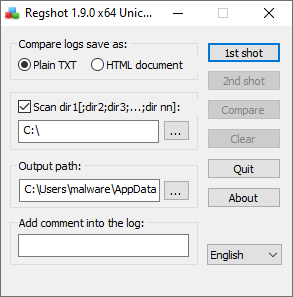
\includegraphics[width=0.4\textwidth]{regshot-firstshot}
\caption{Schermata iniziale all'apertura di RegShot. Cliccando su \softwarecommand{1st shot} si può avviare la scansione per generare la prima istantanea.}
\label{fig:regshot-firstshot}
\end{figure}

Prima di avviare la scansione del sistema cliccando su \softwarecommand{1st shot}, è possibile scegliere quali cartelle far scansionare dal software; per personalizzare questa opzione è necessario spuntare \softwarecommand{Scan dir1[;dir2;dir3;...;dir nn]} e scrivere il percorso desiderato. Nel caso della figura \ref{fig:regshot-firstshot} si è deciso di effettuare l'istantanea per tutto il disco C:\textbackslash{} che è sempre l'opzione consigliabile durante l'analisi dinamica di base. \`E possibile anche scegliere il percorso di salvataggio del documento finale con i risultati del confronto modificando \softwarecommand{Output path}, oltre al poter scegliere se il documento deve essere in formato TXT oppure HTML. In figura \ref{fig:regshot-firstshot} si è scelto di salvare il file in formato TXT.

Una volta cliccato su \softwarecommand{1st shot}, RegShot crea la prima istantanea al termine della quale risulterà selezionabile il tasto \softwarecommand{2nd shot} per effettuare la seconda istantanea come in figura \ref{fig:regshot-secondshot}. Ovviamente tra la prima e la seconda istantanea bisogna eseguire il malware e stare attenti a non effettuare altre operazioni che non siano l'avvio della seconda scansione per non inquinare i risultati finali. 

\begin{figure}[H]
\centering
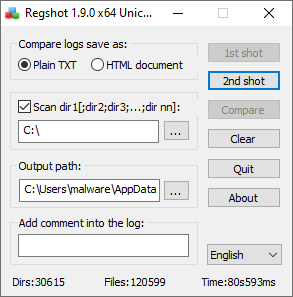
\includegraphics[width=0.4\textwidth]{regshot-secondshot}
\caption{Schermata di RegShot al termine della prima scansione. Il tasto \softwarecommand{1st shot} è selezionabile e cliccandolo si può avviare la scansione per generare la seconda istantanea.}
\label{fig:regshot-secondshot}
\end{figure}

Quando è stata completata anche la seconda scansione il tasto \softwarecommand{Compare} diventa selezionabile e cliccandolo si potrà visualizzare il documento di testo finale che mostra i cambiamenti rilevati.\\

Il documento finale avrà la forma... forma documento ed esempio per un malware.

\section{Behavioural Monitoring}
Tecnica che permette di intercettare in tempo reale i momenti in cui un processo in esecuzione compie determinate azioni, come utilizzare delle funzioni nelle API di Windows oppure accedere e modificare delle chiavi di registro.

Un modo per utilizzare questa tecnica è concentrarsi sul trovare i momenti in cui un processo accedere una serie di operazioni chiave come \strings{WriteFile} o \strings{RegSetValue}, oppure determinati processi come \strings{Process Create}.

Con questa tecnica si possono intercettare i file temporanei non visibili con la tecnica del System Integrity Monitoring, ma non si possono comunque identificare le modifiche a livello del kernel compiute da rootkit.

\subsection*{\softwarename{Process Monitor}}
Process Monitor (o ProcMon) è uno strumento fornito da Windows utilizzato per effettuare il Behavioural Monitoring in tempo reale.

Una volta avviato Process Monitor come amministratore il programma inizierà da subito a registrare tutti gli eventi che accadono nel sistema di tutti i processi attivi, come mostrato in figura . Per focalizzarci solo sugli eventi generati da un certo malware dobbiamo impostare dei filtri e bloccare il monitoraggio nei momenti in cui non ci serve: in questo modo avremmo dei risultati più specifici e accurati.

\begin{figure}[H]
\centering
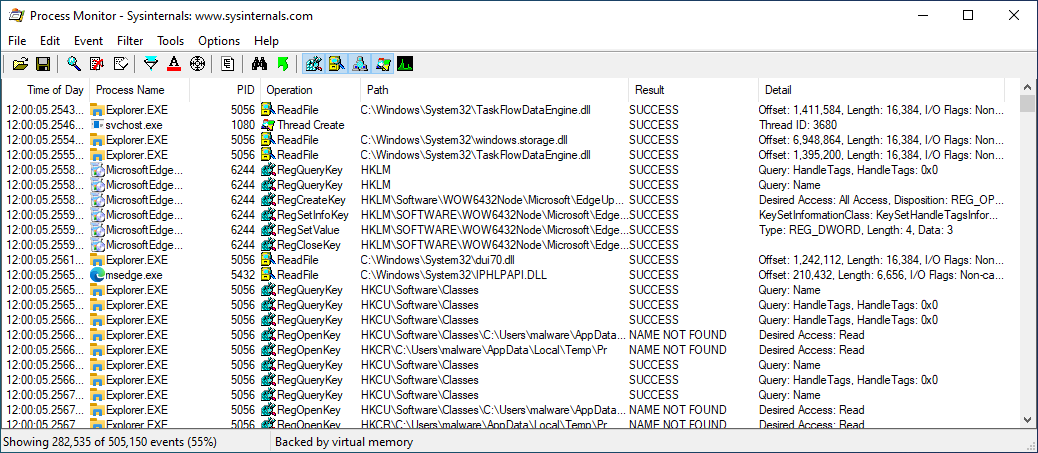
\includegraphics[width=0.98\textwidth]{procmon-main}
\caption{Schermata iniziale all'avvio di Process Monitor senza nessun filtro impostato. Il software, come si può vedere dalla figura, inizia subito a raccogliere tutti gli eventi del sistema.}
\label{fig:procmon-main}
\end{figure}

I filtri su Process Monitor sono impostabili cliccando sul tasto ? e, una volta aperta una nuova finestra, selezionando il tipo di filtro, la relazione e il nome dell'operazione come mostrato in figura . Il primo filtro da impostare, che è anche il filtro principale è il nome del processo malevolo generato dall'esecuzione del malware e si può selezionare come asserzione \textbf{Process Name is malware.exe}, con malware.exe il nome del processo in analisi. Altri filtri che si possono tipicamente settare sono riassunti nella tabella .\\
Operation is WriteFile\\
Operation is RegSetValue\\
Operation is Process Create\\
Operation is SetDispositionInformationFile\\
Operation begins with TCP\\

La figura \ref{fig:procmon-filters} mostra un esempio di impostazione dei filtri principali mostrati nella tabella.

\begin{figure}[H]
\centering
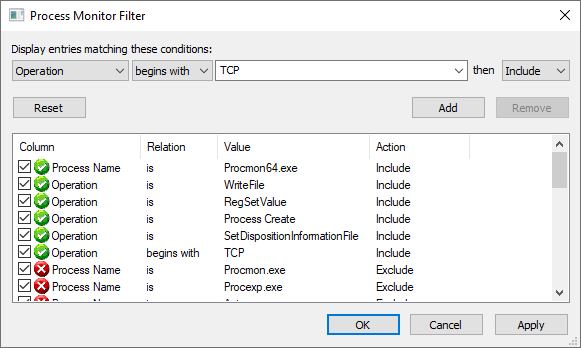
\includegraphics[width=0.7\textwidth]{procmon-filters}
\caption{...}
\label{fig:procmon-filters}
\end{figure}

Per utilizzare Process Monitor in maniera pratica ed analizzare il comportamento di un malware, per prima cosa, oltre ad aver impostato i filtri, bisogna fermare la cattura cliccando sull'icona ? che diventerà ? e starà ad indicare che in quel momento non si stanno più registrando eventi. Per pulire la memoria di Process Monitor da tutti gli eventi registrati fino ad ora cliccare sull'icona ? . A questo punto si deve riattivare la cattura ed eseguire il malware da analizzare, aspettando un po' di tempo per lasciare che il malware esegua le proprie funzioni. Supponiamo, ad esempio, di eseguire un malware chiamato \textit{budget-report.exe} che si maschera da file PDF.

Dopodichè fermare la cattura ed aggiungere ai filtri il nome del processo malware: in questo caso il filtro sarà \textbf{Process Name is budget-report.exe}. Si ha quindi il risultato di tutte le azioni filtrate compiute dal malware sul sistema, come in figura \ref{fig:procmon-analysis1}.

\begin{figure}[H]
\centering
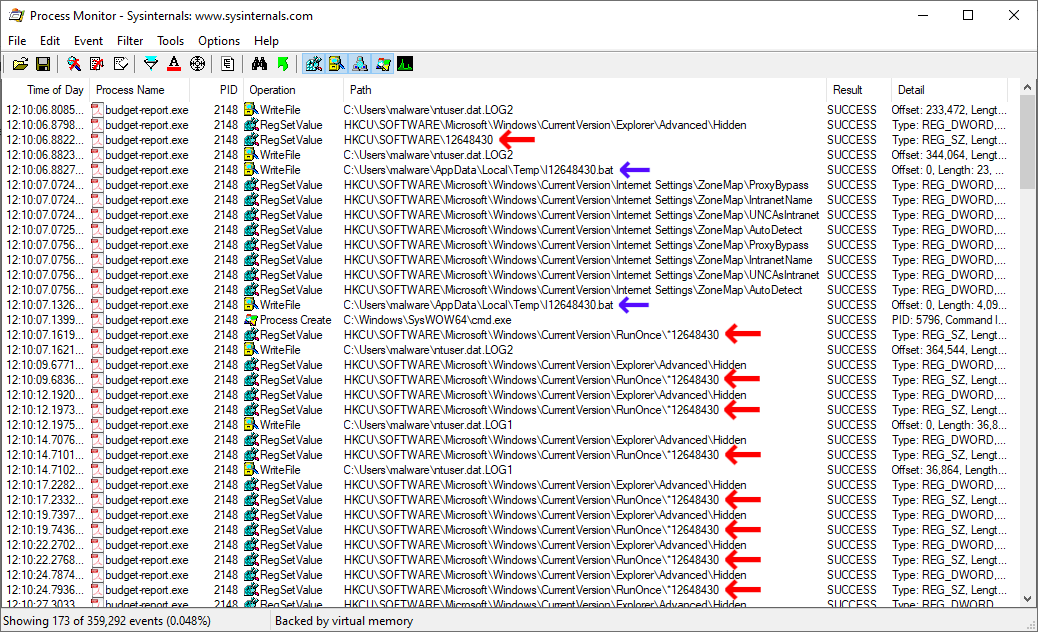
\includegraphics[width=0.98\textwidth]{procmon-analysis1}
\caption{Risultato parziale dell'analisi degli eventi registrati dal malware budget-report.exe. Si può notare nelle righe indicate dalle frecce rosse che il malware agisce sulle chiavi di registro per crearsi una persistenza, mentre nelle righe indicate dalle frecce blu che il malware ha creato dei file temporanei durante la sua esecuzione.}
\label{fig:procmon-analysis1}
\end{figure}

Il malware per prima cosa scrive su un file chiamato \strings{ntuser.dat.LOG2} e si crea una chiave di registro con un proprio numero identificativo\\
\hspace*{1.0cm}\strings{HKCU\textbackslash{}SOFTWARE\textbackslash{}12648430}\\
ed accede ad un altra chiave di registro\\
\hspace*{1.0cm}\strings{HKCU\textbackslash{}SOFTWARE\textbackslash{}Microsoft\textbackslash{}Windows\textbackslash{}CurrentVersion\textbackslash{}Explorer\textbackslash{}Advanced\textbackslash{}Hidden}\\
per modificarne il valore da 4 a 2. Quest'ultima chiave gestisce la visualizzazione di file nascosti su Windows quindi si può dedurre che il malware adotti strategie per nascondersi.\\

Le funzionalità principali di questo malware, mostrate anche in figura \ref{fig:procmon-analysis1}, sono il raggiungimento della persistenza sulla macchina della vittima, che gli garantisce l'esecuzione ad ogni accesso dell'utente. Oltre alla persistenza è importante notare anche la creazione e scrittura di file temporanei (indicati in figura \ref{fig:procmon-analysis1} con delle frecce blu) che non saremmo in grado di rilevare con un analisi di tipo System Integrity Monitoring.\\

Su Process Monitor è anche possibile visualizzare informazioni sugli eventi come le chiavi di registro modificate e il nuovo valore impostato, basta fare doppio click sulla chiave di registro. La figura \ref{fig:procmon-analysis1-event} mostra la finestra di dettaglio di un'operazione di RegSetValue.

\begin{figure}[H]
\centering
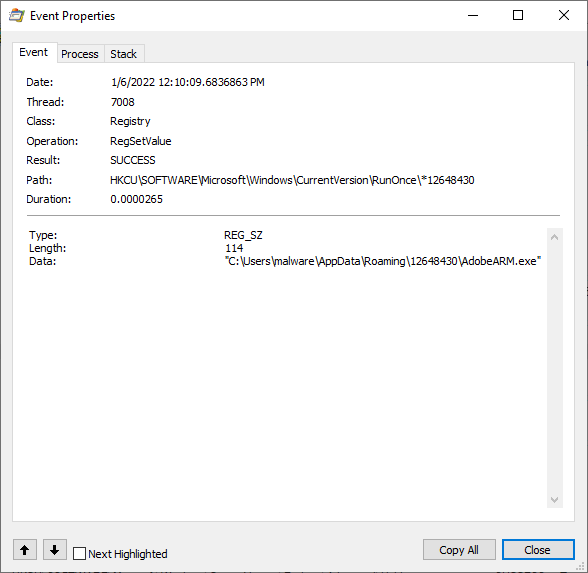
\includegraphics[width=0.5\textwidth]{procmon-analysis1-event}
\caption{}
\label{fig:procmon-analysis1-event}
\end{figure}

\section{Altri strumenti utili per l'analisi dinamica di base}

\subsection{Simulare la presenza di una rete}
Può capitare che alcune tipologie di malware cerchino di capire se il computer sul quale sono installati sia connesso alla rete oppure no, in questo modo possono evitare di eseguire alcune operazioni e mettere in difficoltà gli analisti che effettuano analisi di base. Per questo esistono degli strumenti che servono a simulare del traffico di rete e far credere ai processi in esecuzione sulla macchina che è presente una connessione ad Internet.
\subsection*{\softwarename{FakeNet}}
FakeNet è uno strumento utilizzato per simulare la presenza di una rete in un ambiente in cui la rete è stata disattivata. 

Avviando FakeNet come amministatore si aprirà un Prompt dei Comandi come quello in figura \ref{fig:fakenet-main} che segna le operazioni compiute da FakeNet.

\begin{figure}[H]
\centering
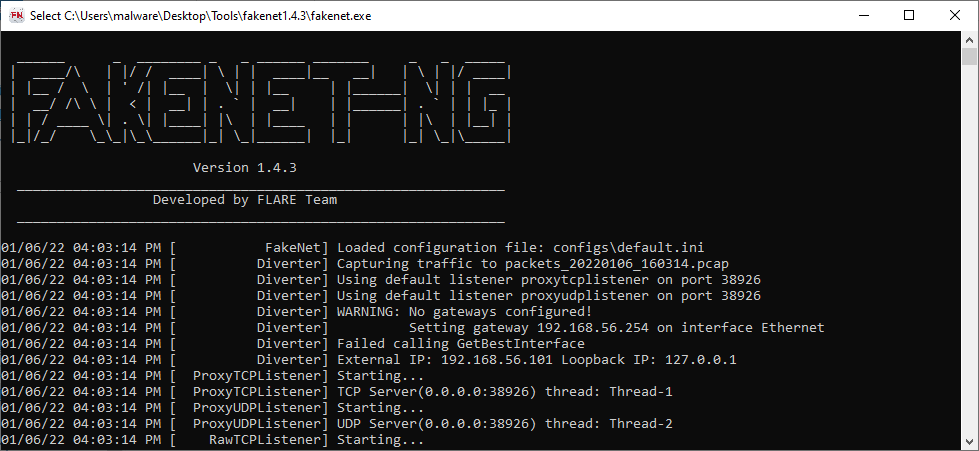
\includegraphics[width=0.8\textwidth]{fakenet-main}
\caption{Prompt dei Comandi visualizzato all'apertura di FakeNet.}
\label{fig:fakenet-main}
\end{figure}

\subsection*{\softwarename{InetSim}}
InetSim è un semplice strumento da linea di comando che può essere lanciato da terminale. Siccome questo strumento viene sviluppato solo per sistemi Linux si consiglia di avviare una macchina virtuale aggiuntiva alla macchina Windows e connettere entrambe le macchine ad una rete interna (sarà comunque spiegato nella prossima sezione).\\
Si può avviare semplicemente con il comando:\\
\shellcommand{sudo inetsim}
Le configurazioni di InetSim sono modificabili con il comando\\
\shellcommand{sudo nano /etc/inetsim/inetsim.conf}
in cui è possibile scommentare le righe che interessano e salvare il file con \scommand{Ctrl+O} e uscire con \scommand{Ctrl+X}.

\section{Come effettuare un'analisi dinamica di base completa}
Per effettuare una analisi dinamica di base completa, utilizzando tutti gli strumenti descritti finora nel capitolo, si deve seguire una precisa procedura. I passi da seguire sono:
\begin{enumerate}
\item Avviare FakeNet;
\item Aprire Process Monitor e fermare la cattura;
\item Creare la prima istantanea del sistema con RegShot;
\item Riprendere la cattura di Process Monitor;
\item Eseguire il malware e aspettare qualche minuto;
\item Fermare la cattura di ProcessMonitor;
\item Creare la seconda istantanea del sistema con RegShot e compararle;
\item Applicare i filtri a Process Monitor e visualizzare i risultati;
\end{enumerate}

...importante seguire l'ordine perchè...

\subsection{Analisi del traffico di rete}
Si può anche utilizzare un metodo alternativo a FakeNet per simulare un'attività di rete e nel contempo effettuare una cattura dei pacchetti per monitorare le connessioni ad internet del malware.


%%%%%%%%%%%%%%%
%% analisi statica avanzata
\chapter{Analisi statica avanzata}

I malware vengono scritti generalmente in linguaggi di programmazione ad altro livello, la maggior parte in C o C++ e vengono compilati da un compilatore che genera un file EXE. Questo file EXE è essenzialmente una sequenza di byte. Guardando il codice macchina si vede che i byte in esadecimale sono rappresentati da due cifre, quindi ci si trova davanti a contenuti del tipo:

... esempio sequela di esadecimali

Per effettuare l'analisi statica avanzata ed analizzare il codice partendo da istruzioni binarie si ricorre al cosiddetto \textit{Reverse Engineering}.

\section{Reverse Engineering}
Il Reverse Engineering può essere definito come l'arte di identificare algoritmi e strutture dati ad alto livello nel linguaggio Assembly. Si definiscono le funzionalità del malware, si guardano le variabili globali utilizzate e si cerca di definire un profilo del malware.\\
Con il Reverse Engineering ci possiamo accorgere di comportamenti particolari da parte del malware come andare a vedere sulla macchina della vittima quali software sono installati e quali dati possono essere inviati sulla rete. Possiamo anche visualizzare delle istruzioni o dei dati che sono stati codificati per essere nascosti e ricercare la funzione, che altrimenti non sarebbe possibile visualizzare con l'analisi di base.
\subsection{Processo di Reverse Engineering}
Il processo del Reverse Engineering si divide in 9 passi:
\begin{enumerate}
\item Identificare se il malware è impacchettato;
\item Effettuare un'analisi statica di base;
\item Effettuare un'analisi dinamica di base;
\item Disassemblare il codice;
\item Identificare la funzione \strings{main()};
\item Analizzare stringhe e API;
\item Analizzare le funzioni;
\item Aggiungere commenti o etichette alle istruzioni e rinominare funzioni e variabili;
\item Analizzare il codice che contiene riferimenti al codice già analizzato;
\item Ripetere i passi 5-7 se necessario. 
\end{enumerate}

La prima cosa importante è proprio capire da subito se il malware è stato impacchettato oppure no, e nel caso lo fosse bisogna tentare di spacchettarlo. Con un eseguibile impacchettato infatti non si riuscirebbe ad eseguire alcuna analisi precisa del suo comportamento. Con il malware spacchettato si eseguono innanzitutto le analisi statica e dinamica di base per identificare le stringhe e le librerie importate che possono essere associate ad azioni malevoli, e si raccolgono informazioni circa la sua esecuzione nel sistema operativo, quali modifiche esegue e se effettua operazioni con la rete (si vedano i capitoli precedenti).\\

Una volta compiute le prime due analisi è il momento di passare al disassemblaggio vero e proprio del malware compilato.
Il disassemblaggio avviene tramite appositi software che forniscono delle interfacce per navigare all'interno delle istruzioni in Assembly e suddividono il codice in funzioni (subroutine). Alcuni software, che verranno descritti all'interno di questo capitolo, sono IDA e Ghidra.\\

Il primo passo da eseguire una volta disassemblato il codice è identificare la funzione \strings{main()} da cui partire ad analizzare il codice, dopodichè successivamente cercare di dare un significato alle stringhe presenti e alle librerie importate, cercando di capire come vengono utilizzate e dove.\\

Dopodichè cercare di analizzare le funzioni presenti facendo lo stesso procedimento logico delle stringhe. In particolare ci si deve porre alcune domande e cercare il più possibile di dare una risposta per ogni funzione di interesse:
\begin{itemize}
\item Quant è complessa la funzione?
\item Ha variabili locali?
\item Ha degli argomenti?
\item Quali altre funzioni la chiamano e quali funzioni chiama?
\item Quali sono le principali strutture di controllo?
\end{itemize}

Importante, una volta compreso il significato di ciò che si è analizzato, è commentare per non dimenticarsi ad una successiva rianalisi. Tipicamente gli strumenti per il Reverse Engineering permettono di aggiungere commenti alle righe di codice o rinominare alcune funzioni con un nome più evocativo delle loro funzionalità. In questo modo, analizzando dell'altro codice successivamente che contiene riferimenti al codice già analizzato, sarà più semplice farsi un'idea del funzionamento generale del malware. Spesso è necessario ripetere le analisi delle stesse istruzioni più volte.

\subsection{General Stack Frame}
da riguardare

\subsection{Riconoscere le funzioni in Assembly}
\subsubsection*{main()}
La funzione main solitamente si trova verso la fine della funzione start ed è formata da tre PUSH seguite da una CALL ad una funzione. Un esempio di main() è:
\begin{Verbatim}
push eax
push edi
push dword prt [esi]
call sub_401040
\end{Verbatim}

\subsubsection*{Argomenti e variabili di una funzione}

\subsubsection*{Funzioni delle API di Windows}
\begin{Verbatim}[commandchars=\\\{\}]
HINTERNET \textcolor{blue}{InternetOpenA}(
    [in] LPCSTR lpszAgent,
    [in] DWORD  dwAccessType,
    [in] LPCSTR lpszProxy,
    [in] LPCSTR lpszProxyBypass,
    [in] DWORD  dwFlags
);
\end{Verbatim}
\begin{Verbatim}[commandchars=\\\{\}]
push 0              \textcolor{blue}{; dwFlags}
push 0              \textcolor{blue}{; lpszProxyBypass}
push 0              \textcolor{blue}{; lpszProxy}
push 0              \textcolor{blue}{; dwAccessType}
push offset szAgent  \textcolor{blue}{; "Internet Explorer 7.5/pma"}
call ds:\textcolor{magenta}{InternetOpenA}
\end{Verbatim}

\subsubsection*{printf()}
Riconoscere all'interno del codice le funzioni printf(), cioè le funzioni che stampano a video un messaggio, è più complicato del main(). Di solito l'istruzione CALL che chiama la funzione printf() è preceduta da un PUSH che rappresenta l'argomento da passare, inserito nello stack. Questo PUSH è nella forma: \scommand{push offset <loc\_stringa>}. La parola \scommand{offset} indica che viene passato l'indirizzo della stringa e non direttamente la stringa, come di norma per le funzioni printf() del linguaggio C.\\

Un esempio di codice in cui è presente la chiamata alla funzione printf() è
\begin{Verbatim}
push offset aSuccessInterne          ; "Success: Internet Connection\n"
call sub_40105F
\end{Verbatim}
in cui la funzione \scommand{sub\_40105F} è proprio la funzione printf() e \scommand{aSuccessInterne} è dove si trova la stringa da passare come parametro. Come si può notare dall'esempio, alcuni software per disassemblare il codice aggiungono automaticamente un commento nelle righe in cui sono presenti delle allocazioni a stringhe: in questo caso vediamo che la stringa in questione è \strings{Success: Internet Connection\textbackslash{}n}.

\subsubsection*{Incremento di un contatore}
\begin{Verbatim}
mov eax [ebp+var_4]
add eax 1
mov [ebp+var_4] eax
\end{Verbatim}

\subsubsection*{Stringhe}

\section{Strumenti per il Reverse Engineering}

\subsection*{\softwarename{IDA Freeware}}
IDA è un software utilizzato nell'ambito del Reverse Engineering e permette il disassemblaggio di un file eseguibile, ovvero permette di risalire alle istruzioni Assembly di cui è composto. Esistono tre versioni di IDA: \textit{Pro}, \textit{Freeware} e \textit{Demo}. La versione Pro permette di disassemblare non solo file eseguibili EXE di Windows ma anche file eseguibili per Linux e altri formati. La versione Freeware invece permette solo il disassemblaggio di eseguibili Windows in 32 bit e 64 bit. Per semplicità qui di seguito verrà descritto l'utilizzo della versione Freeware.\\

Per iniziare bisogna aprire IDA e cliccare su \softwarecommand{New} per scegliere un file da disassemblare. Una volta fatto dovremmo trovarci davanti ad una schermata come quella in figura \ref{fig:ida-main}.

\begin{figure}[H]
\centering
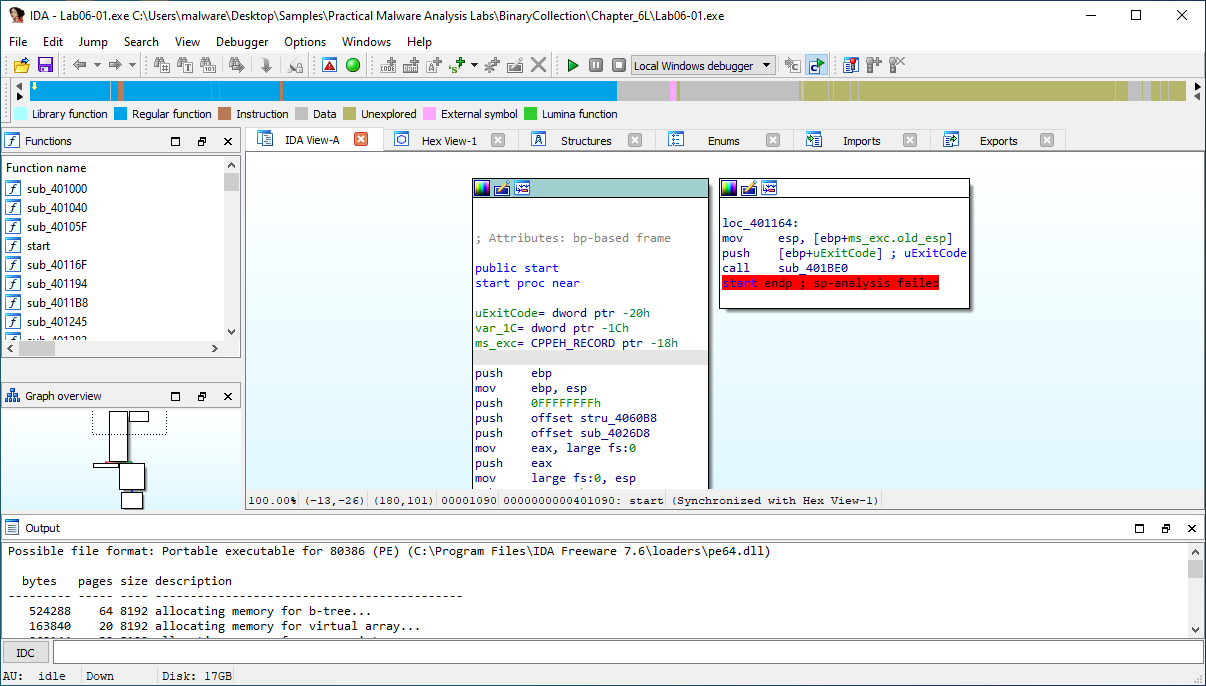
\includegraphics[width=0.9\textwidth]{ida-main}
\caption{Schermata iniziale di IDA Freeware all'apertura di un file eseguibile EXE.}
\label{fig:ida-main}
\end{figure}

IDA è composto da una finestra centrale in cui è possibile visualizzare il codice disassemblato in due forme: o in \textit{modalità grafo}, dove viene mostrato il codice come una sorta di diagramma di flusso, oppure in \textit{modalità testuale}, mostrando le istruzioni riga per riga. Per passare da una modalità all'altra si può premere la barra spaziatrice oppure cliccare il tasto destro e selezionare \softwarecommand{Graph View} o \softwarecommand{Text View}.

Quando viene aperto un file, IDA simula il caricamento in memoria del file e si posiziona sul punto del codice in cui partirebbe la memoria. Con la modalità testo è possibile vedere per ogni riga di istruzioni la sezione dell'eseguibile in cui è presente in memoria (per esempio \textbf{.text}) e il possibile indirizzo di memoria in cui verrebbe allocato.\\

Nella modalità grafo, il codice viene organizzato in modo che ad ogni JUMP (\scommand{jmp}) condizionale vengono visualizzati nel diagramma due possibili percorsi a due blocchi: uno collegato con una freccia verde che indica il caso in cui la condizione della jump è verificata e uno collegato ad una freccia rossa che indica il caso in cui la condizione della jump non è verificata. I blocchi di istruzioni sono separati anche nel caso di call ad una routine o nel caso di loop dove troviamo delle freccie blu che tornano ad un blocco precedente. Nel caso della modalità testuale si può trovare la divisione delle routine del codice per la presenza di linee tratteggiate nel lato sinistro delle istruzioni, mentre le JUMP che soddisfano le condizioni sono unite da linee continue, sempre a lato del codice.\\

La finestra \softwarecommand{Functions}, che solitamente si trova nella parte sinistra all'interno della finestra di IDA, mostra tutte le funzioni (o subroutine) presenti nel codice e selezionandole è possibile collocarsi automaticamente sulla parte di codice dove inizia quella funzione. La finestra di \softwarecommand{Output} in basso mostra alcune informazioni sul caricamento del codice.\\

Altre finestre interessanti sono quelle presenti accanto alla finestra dove è contenuto il codice. Ad esempio \softwarecommand{Imports} mostra le funzioni importate dal malware e il loro indirizzo di memoria, mentre \softwarecommand{Exports} mostre eventuali librerie esportate. \`E possibile anche visualizzare le stringhe presenti nell'eseguibile con la finestra \softwarecommand{Strings} (se la finestra non è presente la si può inserire da \softwarecommand{View} > \softwarecommand{Open subviews} > \softwarecommand{Strings}). La finestra \softwarecommand{Hex View-1} mostra il codice che si sta analizzando come sequenze di byte in esadecimale insieme ad una decodifica in caratteri ASCII.

\subsubsection{Analizzare il codice con IDA Freeware}
All'avvio di IDA, le istruzioni verranno mostrate a partire da una funzione chiamata \strings{start} che corrisponde alla AddressOfEntryPoint (? o qualcosa di simile) e non corrisponde alla funzione \strings{main} (che bisogna trovare manualmente come descritto in precedenza). Selezionando una funzione dalla lista nella finestra \softwarecommand{Functions} spesso è possibile visualizzare la lista delle variabili utilizzate nella funzione e degli argomenti della funzione tipicamente identificate rispettivamente come \scommand{var\_xx} e \scommand{arg\_xx}, con \strings{xx} offset rispetto al puntatore sullo stack; per variabili utilizzate per le chiamate a librerie importate note IDA riesce ad assegnargli il nome della libreria. La figura \ref{fig:ida-variables} mostra un esempio di variabili e argomenti di una funzione.

\begin{figure}[H]
\centering
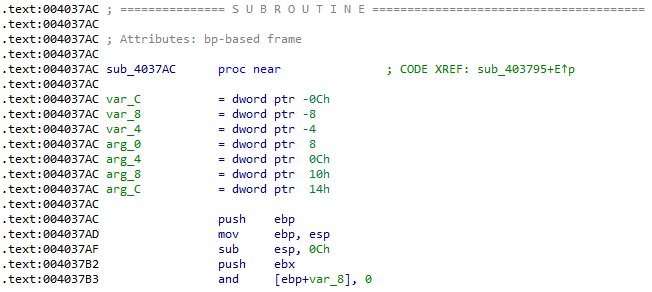
\includegraphics[width=0.9\textwidth]{ida-variables}
\caption{Visualizzazione in IDA Freeware delle variabili e degli argomenti di una funzione chiamata \scommand{sub\_4037AC} nella modalità testuale. In questo caso le variabili contenute nella funzione sono 3: \scommand{var\_C}, \scommand{var\_8} e \scommand{var\_4}, mentre gli argomenti passati alla funzione sono 4: \scommand{arg\_0}, \scommand{arg\_4}, \scommand{arg\_8} e \scommand{arg\_C}.  Il commento all'inizio \strings{Attributes: bp-based frame} è stato inserito da IDA e indica che gli offset dei nomi delle variabili e argomenti sono riferiti al registro EBP.}
\label{fig:ida-variables}
\end{figure}

Tipicamente valori come \scommand{var\_4} e \scommand{var\_8} significano che la prima variabile sarà accessibile attraverso il registro EBP con un offset di $-4$ e la seconda sarà accessibile con un offset di $-8$. Per gli argomenti delle funzioni invece un valore come \scommand{arg\_0} sarà accessibile con un offset dall'EBP di $+8$ e \scommand{arg\_4} con un offset di $+12$.
Quando in un istruzione troviamo la parola \scommand{offset} significa che si riferisce all'indirizzo di memoria e non al valore all'indirizzo di memoria. Ad esempio:\\
\shellcommand{push offset stru\_4060B8} dove \scommand{stru\_4060B8} è una variabile globale, significa che non si andrà a salvare il valore della variabile globale ma il suo indirizzo.

\`E possibile assegnare un nome a variabili e funzioni che posso identificare con determinati comportamenti a cui, per praticità, voglio dare un nome evocativo. Posso farlo cliccando sulla variabile o la funzione selezionata e premere la lettera \softwarecommand{N} oppure con il tasto desto cliccare su \softwarecommand{Rename}; si aprirà una finestra in sovraimpressione che mi permetterà di assegnare un nome che verrà mantenuto per ogni ricorrenza all'interno del file. Si possono inoltre aggiungere dei commenti ad ogni riga premento il tasto \softwarecommand{:} oppure con il tasto destro selezionando \softwarecommand{Enter comment...}.\\

Per posizionarsi all'indirizzo di una determinata funzione e poterla visualizzare si può semplicemente selezionarne il nome con il mouse e premere la lettera \softwarecommand{G}, fare doppio click oppure anche premere il tasto destro e selezionare \softwarecommand{Jump to operand}. Per tornare alla posizione precedente si può cliccare la freccia blu che va verso sinistra nella barra degli strumenti in alto. Se si vuole invece vedere la lista di tutti i riferimenti di una funzione ovvero tutti gli indirizzi dei punti in cui è stata chiamata si può selezionare con il mouse la funzione e premere \softwarecommand{X} oppure con il tasto destro selezionare \softwarecommand{Jump to xref to operand...} e si visualizzarà un lista dei riferimenti. Andando inoltre al punto in cui viene dichiarata una funzione o una variabile, IDA mostra un commento che indica il riferimento nella forma \scommand{[DATA|CODE] XREF: <function><offset>[$\uparrow$|$\downarrow$]<type>}, per esempio:\\
\shellcommand{sub\_401000		; CODE XREF: sub\_401040+4$\downarrow$p}
significa che la funzione sub\_401000 è richiamata dalla funzione sub\_401040 all'offset +4 dall'indirizzo della funzione. Un'esempio simile si può notare anche nel codice all'interno della figura \ref{fig:ida-variables}.  Per una variabile invece un riferimento del tipo:\\
\shellcommand{dword\_409938		; DATA  XREF: start+30$\uparrow$w}
significa che la variabile dword\_409938 è modificata nella funzione start all'offset +30. Il fatto che la variabile venga modificato lo si può capire dalla w alla fine, se ci fosse stato la r sarebbe stata riferita in lettura. IDA può anche mostrare una visualizzazione grafica dei riferimenti ad una funzione selezionata con l'opzione \softwarecommand{View} > \softwarecommand{Open subviews} > \softwarecommand{Proximity browser}. La figura \ref{fig:ida-proximitybrowser} mostra un esempio di questa modalità.

\begin{figure}[H]
\centering
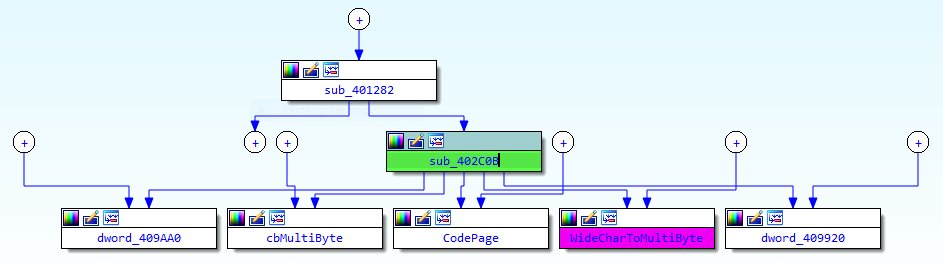
\includegraphics[width=0.98\textwidth]{ida-proximitybrowser}
\caption{Esempio di visualizzazione dei riferimenti per la funzione \scommand{sub\_402C0B}. Si può notare che questa funzione è chiamata da \scommand{sub\_401282}, mentre al suo interno chiama le variabili \scommand{dword\_409AA0}, \scommand{cbMultiByte}, \scommand{CodePage}, \scommand{WideCharToMultiByte} e \scommand{dword\_409920}. Per espandere l'albero a tutte le altre funzioni connesse si può cliccare su i simboli \softwarecommand{+}.}
\label{fig:ida-proximitybrowser}
\end{figure}

I riferimenti possono essere trovati anche per le stringhe: basta cliccare su una stringa da cercare nella finestra \softwarecommand{Strings} e premere la lettera \softwarecommand{X}. Questo mi darà la lista di tutte le funzioni che chiamano quella stringa.

\subsection*{\softwarename{Ghidra}}
Questo software opensource è stato sviluppato dalla NSA (National Security Agency) americana ed è stato pensato per semplificare il processo di reverse engineering del codice. Si differenzia da IDA per la presenza di un compilatore che permette di ricostruire le istruzioni Assembly in codice C. Inoltre Ghidra supporta la creazioni di script tramite i quali è possibile estendere le funzionalità di analisi.\\

La prima cosa da fare una volta aperto Ghidra è creare un nuovo progetto con \softwarecommand{File} > \softwarecommand{New Project}. Il software permette di scegliere se creare un progetto \textit{Non-Shared Project} o \textit{Shared Project}, dove lo Shared Project è un progetto condiviso con più analisti che sono connessi con un Ghidra Server; per lo scopo di questo testo selezionare \softwarecommand{Non-shared Project}. Verrà chiesta la cartella dove salvare il progetto e il nome da dare al progetto. Una volta aperta una schermata di Ghidra con il progetto appena creato, per analizzare un file malevolo bisogna aggiungerlo al progetto cliccando su \softwarecommand{File} > \softwarecommand{Import File}.\\

Ghidra possiede dei cosiddetti \softwarecommand{Tool Chest} visibili nella schermata iniziale del progetto, in particolare tre: l'icona ? per il Reverse Engineering, l'icona ? che permette il debugging e l'icona ? che permette di tracciare le versioni, utile se si lavora su un progetto condiviso.\\

Per eseguire il disassemblaggio del malware ed iniziare le operazioni di Reverse Engineering il file importato e cliccare l'icona ?, oppure fare doppio click. Ghidra chiederà di analizzare il file e la risposta è \softwarecommand{Yes}. A questo punto ci si troverà davanti ad una schermata come quella di figura \ref{}.

\begin{figure}[H]
\centering
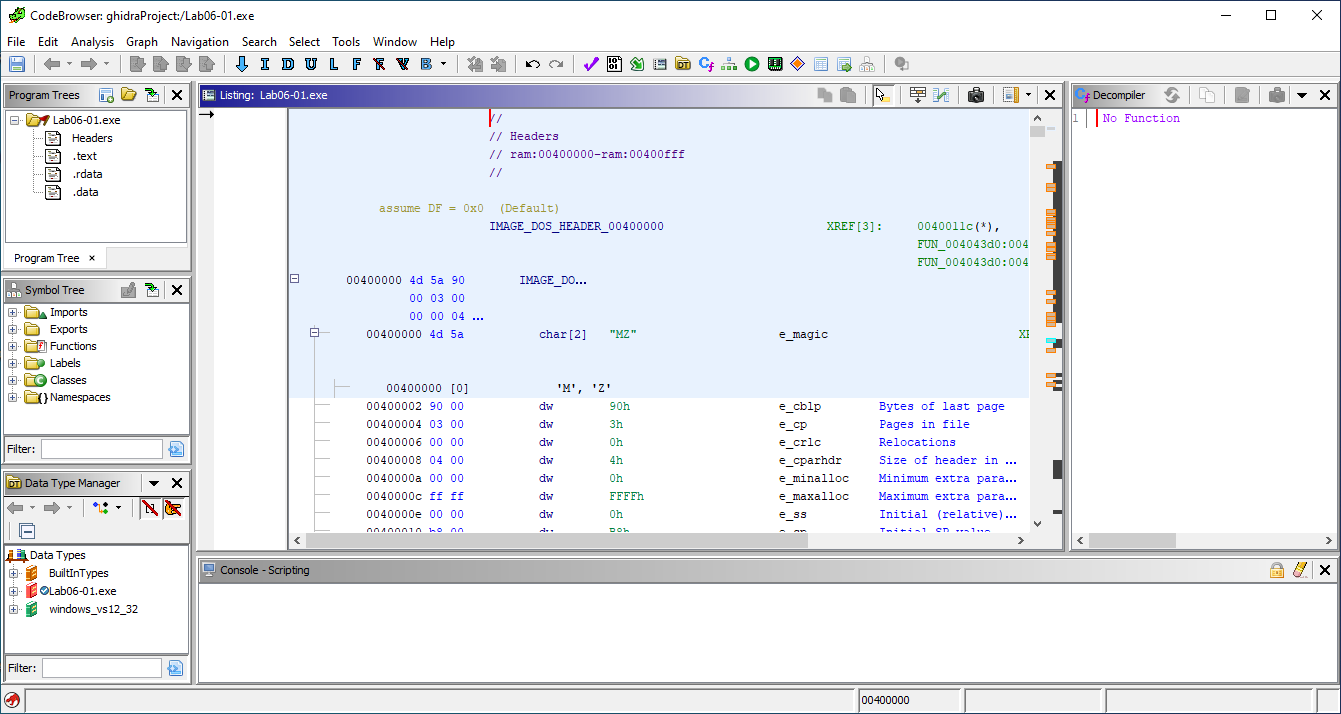
\includegraphics[width=0.98\textwidth]{ghidra-main}
\caption{}
\label{fig:ghidra-main}
\end{figure}

Ghidra, analizzando il file, cercerà di identificare funzioni, variabili globali, array, e in più cercherà di ricostruire il linguaggio C di ogni funzioni in Assembly.\\

Tra le finestre all'interno di Ghidra si trova \softwarecommand{Program Trees} che mostra la struttura del file eseguibile come le sezioni e gli header. Non è molto utile nell'analisi. La finestra \softwarecommand{Symbol Tree} invece dà informazioni sulle funzioni importate e utilizzate dal malware, le funzioni esportate e le funzioni create da chi ha programmato il malware. La finestra \softwarecommand{Data Type Manager} mostra i tipi di dati predefiniti che Ghidra è riusciuto a riconoscere. La figura \ref{} mostra le tre finestre appena descritte.\\

La finestra centrale in Ghidra è la finestra \softwarecommand{Listing} che contiene le istruzioni da analizzare. Al caricamento di un file il primo codice che ci viene mostrato non è il primo codice che viene eseguito, come accade in IDA, ma è letteralmente l'inizio del file. Se si sta analizzando un file PE si vedranno le lettere \strings{M} e \strings{Z} caratteristiche degli eseguibili di Windows.
Per trovare la funzione \scommand{strat} bisogna guardare nella finestra \softwarecommand{Symbol Tree} e cliccare sulla funzione \scommand{entry}, sotto la cartella \scommand{Functions}.

Ghidra permette di personalizzare i campi mostrati nella finestra \softwarecommand{Listing} e scegliere solo cosa mostrare oltre al codice Assembly. Per cambiare le impostazioni standard basta cliccare all'interno della finestra sull'icona ? (\softwarecommand{Edit the Listing Fields}) e compariranno dei bottoni che è possibile attivare o disattivare per aggiungere o togliere colonne.\\

Anche Ghidra permette una visualizzazione a grafo del codice ed è ottenibile selezionando \softwarecommand{Window} > \softwarecommand{Function Graph}. Si otterrà una finestra in sovraimpressione, come quella in figura \ref{}, con il grafo corrispondente al codice in modalità testuale.

\subsubsection*{Analizzare il codice con Ghidra}
Una funzione che può essere utile durante l'analisi è l'evidenziazione di tutte le istruzioni uguali. Ad esempio, si vorrebbe, una volta cliccato con il mouse su una PUSH, evidenziare in giallo tutte le altre PUDH all'interno della funzione in cui ci troviamo. Per farlo cliccare su un istruzione con il tasto centrale del mouse (di solito è la rotellina) ma se si vuole cambiare tasto e impostare, per facilità, il tasto sinistro basta andare su \softwarecommand{Edit} > \softwarecommand{Tool Options} e in \textit{Listing Fields} selezionare \textit{Cursor Text Highlight}. In questa finestra cambiare l'impostazione di \textit{Mouse Button To Activate} con il valore \textbf{LEFT}. Volendo in questa finestra è anche possibile cambiare il colore con cui si mettono in evidenza le istruzioni.

Alla sinistra delle istruzioni possiamo trovare delle frecce che facilitano la comprensione delle JUMP.

Analizzando una certa funzione, per conoscere la lista di funzioni che la chiamano e la lista di funzioni che vengono chiamate al suo interno, bisogna posizionarsi sulla funzione e selezionare \softwarecommand{Window} > \softwarecommand{Function Call Trees} e si aprirà una finestra in basso con due liste: \textit{Incoming Calls} per indicare le funzioni che chiamano la funzione in esame, e \textit{Outgoing Calls} per indicare le funzioni che sono chiamate dalla funzione in esame. Un altro metodo per analizzare i riferimenti è quella dei cross-references che sono solitamente inseriti in una colonna accanto alle istruzioni ed hanno la forma:\\
\begin{Verbatim}
istruzione1		XREF[2]:	00401049(W)
					   0040104c(R)
istruzione2		XREF[1]:	entry:0040113f(c)
\end{Verbatim}
Per l'istruzione 1  si hanno due riferimenti a funzioni che ci accedono: uno dall'istruzione all'allocazione \scommand{00401049} in modalità scrittura (W) e uno da \scommand{0040104c} in modalità lettura (R). Per l'instuzione 2 indica che la funzione in cui ci si trova è stata richiamata da \scommand{entry} all'instruzione presente nell'allocazione di memoria \scommand{0040113f}. L'istruzione 2 tipicamente è il nome di una funzione. La figura \ref{} mostra questo esempio.

\begin{figure}[H]
\centering
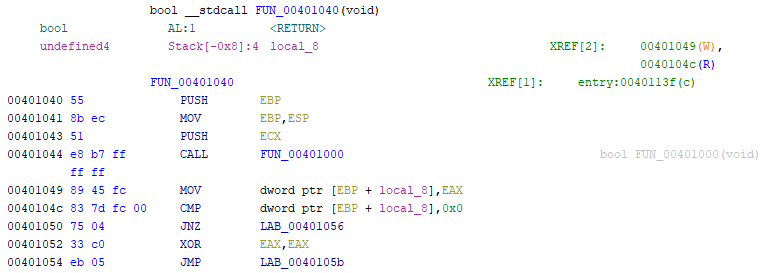
\includegraphics[width=0.98\textwidth]{ghidra-crossreference}
\caption{}
\label{fig:ghidra-crossreference}
\end{figure}

Oltre alla lista dei riferimenti si può anche generare un grafo rappresentante sempre i riferimenti selezionando \softwarecommand{Windows} > \softwarecommand{Function Call Graph}. Si aprirà una nuova finestra in sovraimpressione come quella di figura \ref{fig:ghidra-funcallgraph} dove si può notare che le funzioni sono rappresentate da cerchi e la funzione corrente è evidenziata in giallo, i cerchi che si trovano più in alto della funzione correnti hanno dei riferimenti ad essa (cioè la chiamano), mentre i cerchi che si trovano più in basso sono chiamati dalla funzione corrente.
\begin{figure}[H]
\centering
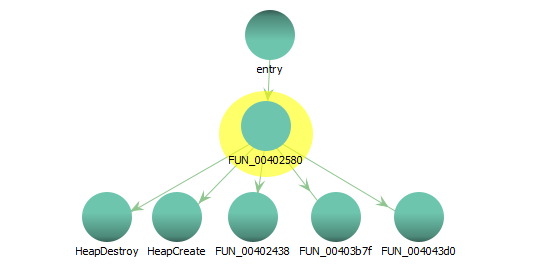
\includegraphics[width=0.75\textwidth]{ghidra-funcallgraph}
\caption{}
\label{fig:ghidra-funcallgraph}
\end{figure}

Per commentare un'istruzione si può cliccare sulla riga dov'è presente l'istruzione e con il tasto destro \softwarecommand{Comments} e selezionare una delle opzioni presenti, che varia in base a dove si vuole che venga posizionato il commento (ad esempio \softwarecommand{Set Post Comment...} posizionerà il commento dopo l'istruzione, mentre \softwarecommand{Set Pre Comment...} lo posizionerà prima).\\

\`E possibile visualizzare tutte le stringhe presenti nel file malevolo selezionando \softwarecommand{Windows} > \softwarecommand{Defined Strings}. Si aprirà una nuova finestra solitamente sulla destra del software che è rappresentata in figura \ref{fig:ghidra-strings}. Si possono visualizzare i nomi delle stringhe con le loro locazioni all'interno del codice e il tipo di dato.

\begin{figure}[H]
\centering
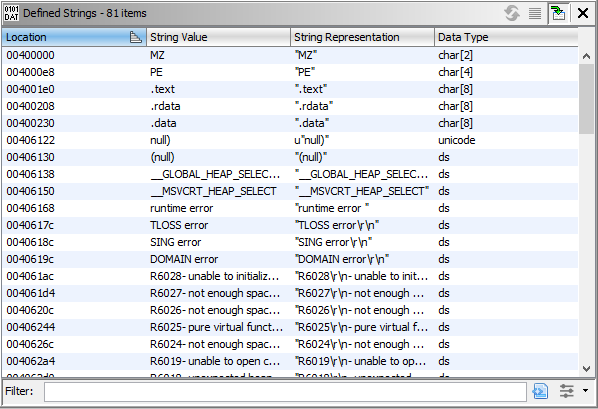
\includegraphics[width=0.7\textwidth]{ghidra-strings}
\caption{}
\label{fig:ghidra-strings}
\end{figure}

\subsubsection*{Decompile}
La funzionalità di \softwarecommand{Decompile} si occupa di decompilare il linguaggio Assembly in linguaggio C. In realtà il passaggio tra i due linguaggi non è diretto ma c'è un passaggio intermedio. Ghidra è in grado di distinguere il linguaggio Assembly dei processori x86 da quelli x86\_64 e così via grazie a dei plugin interni che trasformano tutte le istruzioni in un linguaggio particolare detto \textbf{PCode}, che viene a sua volta trasformato in linguaggio C. Si può visualizzare il codice PCode tramite la finestra \softwarecommand{Listing} > \softwarecommand{Edit the Listing fields} e selezionando una riga di codice cliccare sul tasto destro su \softwarecommand{PCode} e cliccare \softwarecommand{Enable Field}. Accanto alle istruzione comparirà il PCode. Qui di seguito è rappresentato un'esempio di codice Assembly con il corrispondente PCode.
\begin{Verbatim}
PUSH 0x3f8			
				$U2f400:4 = COPY 0x3f8:4
				ESP = INT_SUB ESP, 4:4
				STORE ram(ESP), $U2f400:4
CALL FUN_00403b7f             
				undefined4 FUN_00403b7f(undefine
				ESP = INT_SUB ESP, 4:4
				STORE ram(ESP), 0x4025b9:4
				CALL *[ram]0x403b7f:4
POP ECX					
				ECX = LOAD ram(ESP)
				ESP = INT_ADD ESP, 4:4
JMP LAB_004025c6		
				BRANCH *[ram]0x4025c6:4

\end{Verbatim}

Il codice C corrispondente invece viene mostrato nella finestra \softwarecommand{Decompile} sulla destra del codice e mostra un'interpretazione in linguaggio C della funzione dentro la quale ci si trova. La figura \ref{fig:ghidra-assemblyandc} mostra le due finestre come si presentano.

\begin{figure}[H]
\centering
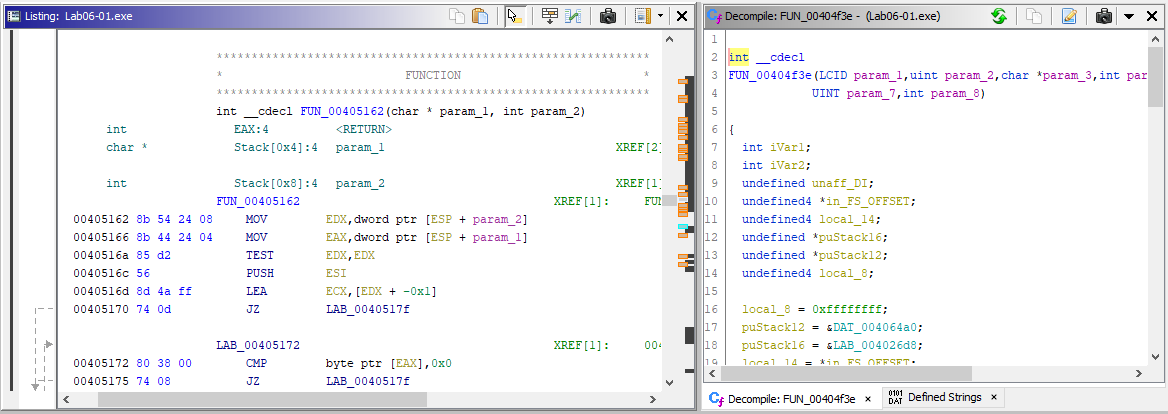
\includegraphics[width=0.98\textwidth]{ghidra-assemblyandc}
\caption{}
\label{fig:ghidra-assemblyandc}
\end{figure}

\`E possibile modificare i dati delle funzioni C per facilitare l'analisi. Per esempio è possibile cambiare alcuni valori come il nome della funzione selezionando la riga di dichiarazione della funzione, oppure anche un'altra funzione qualsiasi, e con il tasto destro cliccare \softwarecommand{Edit Function Signature}.

\subsubsection*{Utilizzo degli script}
Se si clicca sull'icona ?  si aprirà la finestra \softwarecommand{Script Manager} che contiene più di 200 script di Ghidra che possono essere utilizzati per facilitare l'analisi del codice. Gli script sono organizzati in cartelle.\\

Per eseguire uno script basta fare doppio click sul nome e verrà eseguito in Ghidra. Uno script molto utile può essere \strings{RecursiveStringFinder.py} e si può trovare sotto la cartella \softwarecommand{Strings}, e la sua funzione è quella di facilitare l'analisi delle stringhe ricercando ricorsivamente, posizionatisi all'interno di una funzione, tutte le stringhe che si trovano anche nelle funzioni richiamate.
Una volta avviato fornirà tramite la finestra \softwarecommand{Console-Scripting} il risultato della ricerca di tutte le stringhe e il relativo indirizzo di memoria.\\

Lo \softwarecommand{Script Manager} offre anche la possibilità di creare un nuovo script personalizzato che può essere scritto in linguaggio Java oppure Python. Per creare un nuovo script si può cliccare sull'icona ? nella barra in alto a destra. Una volta scelto il linguaggio e assegnato un nome allo script si aprirà una finestra con un editor per modificare il codice.
Ghidra possiede inoltre un interprete Python che esegue ogni istruzione direttamente e si può avviare andando in \softwarecommand{Window} > \softwarecommand{Python}.

\subsubsection*{GhidraDev per Eclipse}
GhidraDev è un plugin che si può installare nell'IDE Eclipse e permette di creare degli script direttamente nell'ambiente di sviluppo di Eclipse, facilitando di molto la scrittura di uno script per Ghidra.

%%%%%%%%%%%%%%%%
%% analisi dinamica avanzata
\chapter{Analisi dinamica avanzata}

\section{Debugging}

\section{Strumenti per l'analisi dinamica avanzata}
\subsection*{\softwarename{x32dbg}}
Il software x32dbg è uno strumento opensource che permette di eseguire i malware in maniera controllata e monitorare come i malware vanno a modificare determinate locazioni di memoria. 

Si inizia eseguendo x32dbg come amministratore e cliccando su \softwarecommand{File} > \softwarecommand{Open} e selezionando il malware da analizzare. Comparirà una schermata come quella in figura \ref{fig:x32dbg-main}. L'esecuzione del malware inizia automaticamente.

\begin{figure}[H]
\centering
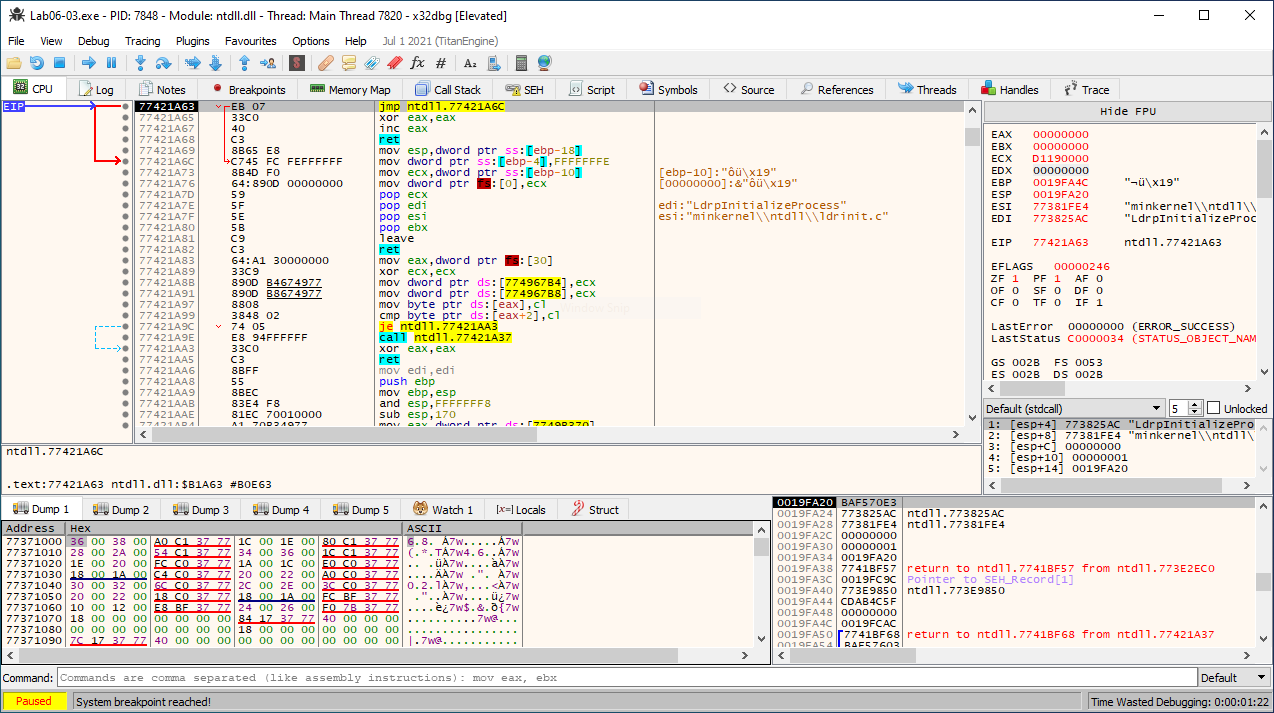
\includegraphics[width=0.98\textwidth]{x32dbg-main}
\caption{}
\label{fig:x32dbg-main}
\end{figure}

La finestra di x32dbg possiede quattro interfacce principali. La prima è una finestra che si trova al centro della finestra principale ed è dove si trova il codice Assembly con le corrispondenti aree di memoria. All'avvio del software il codice viene sospeso su dei breakpoint preimpostati, in particolare vengono inseriti dei breakpoint di sistema, sulla funzione entry e sulle TLS Callback (si veda il capitolo sull'offuscamento). \`E possibile impostare i breakpoint iniziali andando su \softwarecommand{Options} > \softwarecommand{Preferences} > \softwarecommand{Events}. Il codice Assembly è visualizzabile anche in modalità grafo, attivabile premendo la lettera \softwarecommand{G}.\\

La seconda interfaccia è una finestra che si trova a destra della prima ed è una rappresentazione dei registri della CPU e dei loro valori correnti all'indirizzo in cui l'esecuzione è ferma.\\

La terza interfaccia si trova in basso a sinistra ed è una finestra che mostra il \textit{Memory Dump}, ovvero permette di visualizzare il contenuto di diversi indirizzi di memoria.\\

L'ultima interfaccia in basso a destra è una finestra che rappresenta lo stack di memoria, e mostra i valori in riga per ogni indirizzo di una cella di memoria.\\

Una funzionalità molto utile è la scheda \softwarecommand{Memory Map} che si trova nella finestra dove viene mostrato il codice. Rappresenta l'area di memoria che è stata allocata per l'esecuzione del processo. Mostra a quali indirizzi di memoria sono state copiate tutte le sezioni dell'eseguibile, le librerie, ecc... La figura \ref{} mostra una piccola sezione della scheda con alcuni indirizzi di memoria.
\begin{figure}[H]
\centering
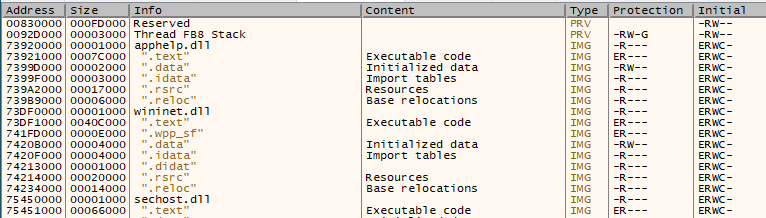
\includegraphics[width=0.98\textwidth]{x32dbg-memorymap}
\caption{}
\label{fig:x32dbg-memorymap}
\end{figure}
Un'altra scheda utile è \softwarecommand{Symbols} che mostra quali sono le le librerie importate dal malware, e cliccando su ogni libreria vengono anche mostrate la lista di funzioni importate appartenenti a quella libreria. La scheda \softwarecommand{References} mostra quelli che possono essere considerati i cross-references. Inizialmente la scheda è vuota e per popolarla bisogna posizionarsi sulla finestra che visualizza il codice Assembly e con il tasto destro cliccare \softwarecommand{Search for} > \softwarecommand{Current Module} > \softwarecommand{Intermodular calls}. Viene mostrato per ogni funzione importata dal malware tutte le funzioni che la richiamano.\\

La scheda \softwarecommand{Threads} mostra la lista dei Thread del processo malevolo. La scheda \softwarecommand{Handles} mostra invece la lista di tutti gli Handle (si veda cos'è un handle nell'appendice di Windows).

\subsubsection*{Debugging del codice}
L'esecuzione del codice avviene immediatamente all'apertura di x32dbg per fermarsi al breakpoint sulla funzione entry. Per continuare con l'analisi e quindi con l'esecuzione del debug vengono forniti dei comandi accessibili nella barra in alto della finestra principale del software. La figura \ref{fig:x32dbg-debugcommand} mostra questi tasti.
\begin{figure}[H]
\centering

\includegraphics[width=0.98\textwidth]{x32dbg-debugcommand}
\caption{}
\label{fig:x32dbg-debugcommand}
\end{figure}
Il tasto con icona 3, è la \softwarecommand{Run} e continua l'esecuzione del programma fino a che non incontra un breakpoint oppure fino a che non termina il programma.
Il tasto con icona 5, è la \softwarecommand{Step Into} che, quando incontriamo una funzione, si posiziona sulla prima istruzione all'interno della funzione e permette di eseguire passo per passo la funzione.
Il tasto con icona 6, è la \softwarecommand{Step Over} che agisce sempre quando si incontra una chiamata ad una funzione, ma in questo caso la si esegue in un unico passo e ci si posiziona sull'istruzione successiva alla chiamata.
Il tasto con icona 9, è la \softwarecommand{Execute Till Return} e serve nei momenti in cui ci si addentra in una funzione in cui ci si rende conto essere troppo complessa. Con questo comando si esce dalla funzione posizionandoci sulla istruzione RET di ritorno e si esegue automaticamente la restante parte della funzione.

Esistono due tipologie di breakpoint: \textit{Software breakpoint} e \textit{Hardware breakpoint}. L'inserimento di un Software breakpoint avviene cliccando a sinistra di una riga di un istruzione dove è presente un cerchio grigio pieno. Cliccando sul cerchio da grigio diventerà rosso e significherà che abbiamo impostato un breakpoint a quell'istruzione; cliccando di nuovo il cerchio diventerà verde e il breakpoint verrà disabilitato; cliccando ancora si rimuoverà completamente. Il problema dei Software breakpoint è che sono vulnerabili alle tecniche di anti-debugging implementate da chi scrive i malware, poichè il breakpoint è implementato con un ulteriore istruzione. Per questo esistono anche gli Hardware breakpoint.\\

La differenza con i Software breakpoint è che gli Hardware breakpoint non utilizzano istruzioni ma vengono impostati su dei registri particolari: sette registri \strings{DR} che vanno da \strings{DR0} a \strings{DR7}. Si possono inserire due tipologie di hardware breakpoint: uno per monitorare il valore di una variabile passata come paramentro di una funzione. Per monitorare una variabile selezionarla e con il tasto destro cliccare \softwarecommand{Follow in Dump}. A questo punto, nella finestra in basso a sinistra, il Memory Dump verrà posizionato all'area di memoria della variabile. Qui è possibile inserire un breakpoint cliccando con il tasto destro su \softwarecommand{Breakpoint} e selezionando la tipologia di hardware breakpoint desiderata. In particolare:
\begin{itemize}
\item Hardware, Access: inserisce un hardware breakpoint per l'accesso in lettura
\item Hardware, Write: inserisce un hardware breakpoint per l'accesso in scrittura
\item Hardware, Execute: inserisce un hardware breakpoint per l'a
\item Memory, Access
\item Memory, Read
\item Memory, Write
\item Memory, Execute
\end{itemize}

La scheda \softwarecommand{Breakpoints} mostra una lista di tutti i breakpoint presenti nel codice e dove sono collocati.

Si possono impostare breakpoint per specifiche funzioni di libreria importate andando sulla scheda \softwarecommand{Symbols} e cliccando con il tasto destro su una funzione selezionare \softwarecommand{Toggle Breakpoint}.

\subsubsection*{Cambiare codice e registri durante l'esecuzione}
Con x32dbg è possibile cambiare il comportamento del malware durante la sua esecuzione. Questa funzionalità può essere utile per esplorare diverse funzioni che altrimenti non verrebbero eseguite oppure per contrastare tecniche di anti-analisi o anti-debugging.\\

Per modificare il valore di un registro, bisogna posizionarsi nella finestra dei registri e selezionare quello che si vuole cambiare, cliccare quindi il tasto destro. La finestra di opzioni mostra alcune opzioni per modificare il valore, tra le quali:
\begin{itemize}
\item \softwarecommand{Modify value}
\item \softwarecommand{Set to 1}
\item \softwarecommand{Increment}
\item \softwarecommand{Decrement}
\item \softwarecommand{Increase 4}
\item \softwarecommand{Decrease 4}
\item \softwarecommand{Push}
\item \softwarecommand{Pop}
\end{itemize}

Possiamo anche modificare le istruzioni Assembly durante l'esecuzione, posizionandosi su una riga di codice e con il tasto destro selezionare \softwarecommand{Binary} > \softwarecommand{Edit}. Una volta fatto si apre una finestra che offre la possibilità di cambiare il codice esadecimale di una istruzione. \`E quindi chiaro che devo conoscere il codice corrispondente dell'istruzione che voglio sostituire. Ad esempio si vuole sostituire l'istruzione \scommand{je} (jump if equal) che ha valore esadecimale \strings{74} con un'istruzione \scommand{jmp} (jump non condizionale) che ha valore \strings{EB}. Una riga di codice con valore \strings{74 14} diventerà quindi \strings{EB 14}. Per applicare in maniera permanente le modifiche apportate sul codice e salvare quindi tutto in un nuovo file si può cliccare sull'icona ? nella barra in altro di x32dbg (ovvero il tasto \softwarecommand{Patches}) e cliccare su \softwarecommand{Patch File}, salvando il file con estensione \strings{.exe}.\\

\subsubsection*{Analisi di un file DLL}
Può capitare che un malware possa caricare durante la sua esecuzione una libreria DLL malevola. Purtroppo non si può analizzare il contenuto della DLL direttamente dal malware ma bisogna analizzarla direttamente. Per farlo bisogna prima aprire con x32dbg una DLL di sistema chiamata \strings{rundll32.exe} come fosse un normale file. Questa DLL si trova al percorso:\\\\
\strings{C:\textbackslash{}\textbackslash{}Windows\textbackslash{}SysWOW64\textbackslash{}rundll32.exe}\\\\
A questo punto bisogna selezionare \softwarecommand{File} > \softwarecommand{Change Command Line} e si aprirà una finestra in sovraimpressione che contiene una stringa con il percorso di \strings{rundll32.exe}. Accanto alla stringa bisogna aggiungere il percorso completo del file DLL malevola da analizzare. Ad esempio:\\\\
\strings{"C:\textbackslash{}\textbackslash{}Windows\textbackslash{}SysWOW64\textbackslash{}rundll32.exe"\hspace{0.3cm}C:\textbackslash{}\textbackslash{}Users\textbackslash{}MioUtente\textbackslash{}malware\textbackslash{}MaliciousDLL.dll}\\\\
e cliccare su \softwarecommand{OK}, poi chiudere completamente x32dbg. Avviare di nuovo x32dbg aprendo sempre il file \strings{rundll32.exe} e, nella scheda \softwarecommand{Breakpoints}, cliccare con il tasto destro \softwarecommand{Add DLL breakpoint} e specificare il nome della DLL malevola. Riavviando una seconda volta x32dbg, riaprendo sempre \strings{rundll32.exe}, l'esecuzione del programma dovrebbe bloccarsi sul breakpoint alla libreria DLL da analizzare.
%%%%%%%%%%%%%%%
%% analisi dei pdf e javascript
\chapter{Analisi di script e documenti}

\section{Analisi di documenti PDF}
\subsection{Struttura di un PDF}
\subsection{Analisi di un PDF}

\section{Analisi di codice Javascript}

%%%%%%%%%%%%%%%%
%% tecniche di offuscamento
\chapter{Tecniche di offuscamento e anti-analisi}

\section{Modifica delle stringhe}
Gli attaccanti possono tentare di rendere difficile l'analisi delle stringhe inserendo all'interno del programma stringhe casuali o di tutt'altro significato volte a far credere che il file non sia un file malevolo.

In alcuni casi possono cifrare delle stringhe per oscurarne il contenuto oppure usare dei sistemi di codifica in base64. L'utilizzo di una codifica in base64 all'interno del malware può essere indicata, tramite l'analisi delle stringhe, dalla presenza di stinghe come ABC...abc...+/. Si faccia riferimento al capitolo 2(?).
Può essere utilizzata anche la codifica XOR. Il problema di utilizzare una codifica XOR è il fatto che, a causa della presenza del carattere nullo alla fine di una stringa, riesco a riconoscere la chiave e recuperare l'intera stringa.

\section{Controllo della connessione}
\begin{Verbatim}
push    0               ; dwReserved
push    0               ; lpdwFlags
call    ds:InternetGetConnectedState
mov     [ebp+var_4], eax
cmp     [ebp+var_4], 0
jz      short loc_40102B
\end{Verbatim}

\section{Data Encoding}
Tecniche adottate per offuscare il codice di alcune funzioni come stringhe o chiamate alle funzioni. Queste tecniche possono essere utilizzate da un malware in diversi scenari: si potrebbe voler nascondere a chi analizza il file il nome di dominio del server di Command And Control oppure nascondere altre stringhe sospette. Un keylogger potrebbe codificare i caratteri che raccoglie dalla tastiera prima di salvarli in un file, in questo modo chi vedrebbe il file non capirebbe immediatamente che contiene tutti i caratteri scritti dalla vittima. Queste tecniche sono utilizzate anche per nascondere eseguibile dentro altri file innocui, come ad esempio un file PE all'interno di un immagine.\\

Esistono diversi tipi di Data Encoding.
\subsection{Cifrari semplici}
I cifrari semplici sono facili da forzare anche con tecniche di brute force. Chi li utilizza non punta sulla segretezza del contenuto ma solo sul rendere l'analisi statica molto più difficile per l'analista. Non necessitano di API ma si possono costruire con operazioni semplici.
\subsubsection*{Cifrario di Cesare}
Ogni lettera dell'alfabeto veniva sostituita con la lettera con si trovava ad una posizione data da un certo scorrimento dell'alfabeto. L'esempio sottostante mostra il funzionamento del Cifrario di Cesare con uno scorrimento di 3.\\
\textbf{Alfabeto originale}: 	\strings{ABCDEFGHIJKLMNOPQRSTUVWXYZ}\\
\textbf{Alfabeto codificato}:	\strings{DEFGHIJKLMNOPQRSTUVWXYZABC}\\
Un testo semplice viene quindi codificato come:\\
\strings{ATTACK AT NON}\\
\strings{DWWDFN DW QRRQ}\\

\subsection{Algoritmo XOR}
Utilizza l'operazione di XOR per codificare un testo. Il suo funzionamento consiste nel prendere una chiave di una certa lunghezza in byte e codifica ciascun byte di un testo che voglio nascondere con lo XOR. Per esempio:\\\\
\textbf{Testo}:		\strings{0100 1000 0100 1001}\\
\textbf{Chiave}:		\strings{0011 1100 0011 1100}\\
\textbf{Risultato}:	\strings{0111 0100 0111 0101}\\

Il problema della cifratura con XOR è che è facilmente invertibile: infatti codificando nuovamente il testo cifrato con la chiave si ottiene il testo iniziale. Infatti:\\\\
\textbf{Risultato}:	\strings{0111 0100 0111 0101}\\
\textbf{Chiave}:		\strings{0011 1100 0011 1100}\\
\textbf{Testo}:		\strings{0100 1000 0100 1001}\\\\
Se la chiave è un singolo byte, con la tecnica del brute force ci sono solamente 256 possibili chiavi.\\

Nell'implementazione dell'algoritmo XOR in un file PE, come mostrato in figura \ref{}, possiamo identificare facilmente la chiave come quel carattere che si ripete continuamente. La ripetizione della chiave è dovuta al fatto che quel byte è stato messo in XOR con il byte nullo.

..figura..

Per questo chi progetta malware cerca di utilizzare delle varianti dell'algoritmo XOR per rendere più difficoltosa la decodifica ed evitare che venga subito riconosciuto dagli analisti. L'algoritmo XOR consiste nell'eseguire lo XOR solamente dei caratteri NON NULLI o che non corrispondono alla chiave. Questi ultimi caratteri vengono quindi saltati dall'algoritmo e non codificati, come mostrato in figura \ref{}. Questo algoritmo è detto anche \textbf{NULL-preserving XOR}.

...figura..

\subsubsection*{Identificare le funzioni XOR durante il Reverse Engineering}
All'interno del codice Assembly possono esserci tre forme di istruzioni XOR:
\begin{enumerate}
\item XOR di un registro con sè stesso, ad esempio \scommand{xor edx edx}, ed è utilizzata per resettare il valore di un registro a zero. Questa istruzione è tipicamente innocua e non viene utilizzata per la codifica XOR.
\item XOR di un registro o una locazione di memoria con una costante, ad esempio \scommand{xor [edx] 0x42}. In questo caso può essere un'applicazione della codifica in XOR e che il valore costante rappresenti la chiave di codifica.
\item XOR di un registro o una locazione di memoria con un diverso registro o locazione di memoria,. Anche in questo caso è molto probabile che si applichi l'algoritmo di XOR, inoltre la chiave non è facilmente identificabile perchè non è immediata.
\end{enumerate}

Se si sta utilizzando uno strumento come IDA o Ghidra per trovare i punti in cui viene eseguita una XOR basta cercare tutte le occorrenze in cui è presente un'istruzione \scommand{xor} ed escludere quelle in cui si resettano dei registri. Spesso i punti in cui le xor vengono utilizzate per codificare un testo ricorrono ciclicamente e questo si può individuare con la modalità grafo di IDA o Ghidra, come mostrato in figura \ref{fig:ida-xor}

\begin{figure}[H]
\centering
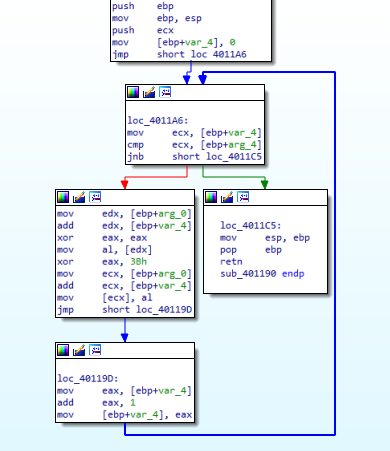
\includegraphics[width=0.4\textwidth]{ida-xor}
\caption{Esempio di codice Assembly mostrato in modalità grafo in cui è visibile un ciclo (mostrato dalla freccia blu) attraverso il quale viene eseguito uno XOR. Questo è un chiaro esempio dell'utilizzo dell'istruzione \scommand{xor} per codificare un testo.}
\label{fig:ida-xor}
\end{figure}

\subsection{Codifica in base64}
Conversione di una stringa in base64. L'algoritmo che codifica in base64 si occupa di prendere 6 bit alla volta e trasformarli in un unico carattere presente nell'alfabeto maiuscolo, minuscolo e nei numberi. In questo modo, la codifica restituisce per ogni 3 byte del testo originale 4 byte del testo codificato. Quando i byte del testo in chiaro non sono divisibili per 3 si aggiungono alla fine della stringa codificata un certo numeri di simboli \strings{=} per compensare. In poche parole i caratteri che si possono trovare in un testo codificato in base 64 è:\\
\strings{A B C D E F G H I J K L M N O P Q R S T U V W X Y Z}\\
\strings{a b c d e f g h i j k l m n o p q r s t u v w x y z}\\
\strings{0 1 2 3 4 5 6 7 8 9}\\
\strings{=}\\

Prendiamo come esempio....

Un malware può utilizzare la codifica in base64 per nascondere le stringhe durante l'analisi statica oppure per nascondere il contenuto di pacchetti che vengono inviati tramite la rete.

\subsubsection*{Identificare la codifica base64 durante l'analisi del malware}
La presenza di codifica in base64 può essere facilmente scovata durante l'analisi statica di base. In particolare se, durante l'analisi delle stringhe, troviamo la stringa:
\strings{ABCDEFGHIJKLMNOP}.\\

Con \softwarename{Krypto ANALyzer}, plug-in di PEiD, si possono trovare le tabelle di codifica di funzioni crittografiche e base64, con accanto l'indirizzo di memoria a cui si trovano.\\

Con strumenti per il Reverse Engineering alcune istruzioni Assembly che indicano una codifica base64 possono essere:
\begin{Verbatim}
cmp [ebx+var_4] 3
...
cmp [ebx+var_4] 4
\end{Verbatim}
Questo perchè l'algoritmo di codifica prevede che il valore di un byte nello stack sia prima confrontato con 3 per capire se è divisibile e successivamente con 4 per capire se vanno aggiunti i simboli \strings{=}. Tra le due istruzioni di compare c'è una jump di qualche tipo.\\

L'analisi dinamica avanzata, ossia l'utilizzo di un debugger, è il miglior modo per decodificare una stringa codificata all'interno del codice.

\subsection{Algoritmi crittografici}
Cifrature simmetriche e asimmetriche.

\subsubsection{Identificazione di algoritmi crittografici}
Si può identificare l'utilizzo di algoritmi crittografici se il malware importa o carica librerie che permettono di implementare la crittografia. Alcune librerie sono:
CryptAcquireContextA
CryptCreateHash
CryptDeriveKey
CryptDestroyHash
CryptDecrypt
CryptEncrypt
Oppure iniziano con, oltre a Crypt, CP o Cert.

Anche l'analisi delle stringhe può essere utile se si trovano stringhe che indicano nomi di protocolli come
OpenSSL
TLSv1
TLSv2
TLSv3
...ecc guardare slide\\

Anche in questo caso può essere utile l'utilizzo di KryptoANALyzer....

\section{Tecniche anti-debugging}
Fanno parte di tecniche anti-analisi e sono specifiche per impedire l'esecuzione del debugging da parte di un analista o per renderlo comunque più difficile. Queste tecniche consistono nell'identificare se il malware è in esecuzione in modalità debug e nel caso deviare il normale corso del programma processando istruzioni diverse da quelle che sarebbero state eseguite in condizioni normali. Ci possono essere centinaia di tecniche differenti e possiamo riassumerle in alcune categorie:
\begin{itemize}
\item Tecniche legate alle API
\item Controllo dei flag
\item Ricerca di processi
\item Controlli basati sul tempo
\item Ricerca di breakpoint
\item Self-debugging
\end{itemize} 

\subsection*{Tecniche legate alle API}
Queste tecniche controllano se l'esecuzione è in modalità debug attraverso librerie e servizi forniti direttamente dal sistema operativo Windows. In particolare si controlla il Process Block Environment (PEB) che mantiene le informazioni relative all'esecuzione del processo, oppure il Thread Environment Block (TEB) che mantiene invece le informazioni riguardanti i thread e al quale appartiene il PEB. Il TEB è una struttura del tipo:
\begin{Verbatim}
typedef struct _TEB {
  PVOID Reserved1[12];
  PPEB  ProcessEnvironmentBlock;	\\ riferimento al PEB
  PVOID Reserved2[399];
  BYTE  Reserved3[1952];
  PVOID TlsSlots[64];
  BYTE  Reserved4[8];
  PVOID Reserved5[26];
  PVOID ReservedForOle;
  PVOID Reserved6[4];
  PVOID TlsExpansionSlots;
} TEB, *PTEB;
\end{Verbatim}
dove si può notare che contiene in effetti un riferimento al PEB, che è una struttura del tipo sottostante:
\begin{Verbatim}
typedef struct _PEB {
  BYTE                          Reserved1[2];
  BYTE                          BeingDebugged;
  BYTE                          Reserved2[1];
  PVOID                         Reserved3[2];
  PPEB_LDR_DATA                 Ldr;
  PRTL_USER_PROCESS_PARAMETERS  ProcessParameters;
  PVOID                         Reserved4[3];
  PVOID                         AtlThunkSListPtr;
  PVOID                         Reserved5;
  ULONG                         Reserved6;
  PVOID                         Reserved7;
  ULONG                         Reserved8;
  ULONG                         AtlThunkSListPtr32;
  PVOID                         Reserved9[45];
  BYTE                          Reserved10[96];
  PPS_POST_PROCESS_INIT_ROUTINE PostProcessInitRoutine;
  BYTE                          Reserved11[128];
  PVOID                         Reserved12[1];
  ULONG                         SessionId;
} PEB, *PPEB;
\end{Verbatim}
All'interno di PEB ci sono tre campi molto importanti, due dei quali non rappresentati dal codice sopra:
\begin{itemize}
\item \scommand{BeingDebugged}: si trova all'offset 0x2 della struttura. Se il valore di questo campo è 1 il processo è eseguito in modalità debug, altrimenti è 0. 
\item \scommand{ProcessHeap}: si trova all'offset 0x18 della struttura.
\item \scommand{NtGlobalFlag}: si trova all'offset 0x68 della struttura.
\end{itemize}

Le API che controllano il valore di \scommand{BeingDebugged} sono \scommand{IsDebuggerPresent}, \scommand{CheckRemoteDebuggerPresent} che, oltre a controllare se il processo corrente è eseguito all'interno di un debugger, controlla anche altri processi poichè prende un Handle come argomento, e infine la \scommand{NtQueryInformationProcess} che può restituire le informazioni sul processo.

Per controllare direttamente il valore di \scommand{BeingDebugged} senza utilizzare un API si può accedere ad un particolare registro \scommand{fs} che punta all'inizio del TEB e accedere al PEB. Il codice può essere di questo tipo:
\begin{Verbatim}
mov eax fs:[30h]          ; accede al PEB
cmp b [eax+2] 0           ; controlla BeingDebugged
jne being_debugged
\end{Verbatim}
dove la prima istruzione memorizza il puntatore al PEB (che si trova all'offset 30h del TEB) nel registro eax, mentre la seconda controlla il valore di BeingDebugger (che si trova all'offset di 0x2 di eax, in questo caso). L'ultima istruzione serve a saltare ad una particolare sezione se il valore di BeingDebugged è maggiore di 0. Per bypassare questa tecnica si possono utilizzare le funzionalità di un debugger come x32dbg per modificare il registro prima che venga effettuta l'istruzione cmp. Oppure sostituire l'istruzione di JUMP con un'istruzione NOP che non fa nulla.\\

Il flag NtGlobalFlag quando viene settato, vengono settati insieme a lui altri tre flag il cui valore totale è 0x70:
\begin{Verbatim}
flag							value
FLG_HEAP_ENABLE_TAIL_CHECK	0x10
FLG_HEAP_ENABLE_FREE_CHECK	0x20
FLG_HEAP_VALIDATE_PARAMETERS	0x40
total							0x70
\end{Verbatim}
Per controllare questo flag direttamente quindi si utilizza un codice Assembly del tipo:
\begin{Verbatim}
mov eax fs:[30h]      ; accede al PEB
mov al, [eax+68h]    ; accede al flag NtGlobalFlag
and al, 70h
cmp al, 70h
je being_debugged
\end{Verbatim}
La prima istruzione, come nel caso di BeingDebugged, accede al PEB, mentre la seconda accede al NtGlobalFlag (che si trova all'offset 0x68 del PEB). Le istruzioni successive calcolano un AND del flag con 70 e poi si controlla che sia 70. Se lo è si salta ad un'altra sezione, come nel caso sopra. Per aggirare questo controllo si applicano le stesse tecniche del caso precedente.\\

Il flag invece, che punta alla struttura del primo Heap che è stato caricato dal System Loader, ha un valore che cambia in base al fatto che l'heap sia stato creato all'interno di un debugger o all'interno del sistema operativo. Al suo interno ha due flag: \scommand{Flags} e \scommand{ForceFlags}. La posizione di questi flag dipende dalla versione del sistema operativo:
nome valore arch
flag: 0x40 32bit
forceflag: 0x44 32bit\\
Le condizioni per il quali si può dire che un processo è eseguito in un debugger sono:
\begin{enumerate}
\item Se il campo \scommand{Flags} non ha il flag \scommand{HEAP\_GROWABLE} impostato al valore 0x00000002;
\item Se il valore di \scommand{ForceFlags} non è 0.
\end{enumerate}
 
Un'altra tecnica molto più banale è cercare le API \strings{FindWindow}, la cui funzione consiste nel cercare una finestra all'interno di Windows che ha un determinato nome. Un esempio di codice che implementa questa tecnica è il seguente:
\begin{Verbatim}
mov edi offset 12
11: push 0
push edi
call FindWindowA
test eax eax
jne being_debugged
or ecx -1
repne scasb
cmp [edi], al
jne 11
\end{Verbatim}
Lo scopo di questa tecnica è nel passare a FindWindowA come argomento il nome della finestra corrente e vedere se corrisponde al nome di qualche famoso debugger in circolazione. Questa tecnica non viene più utilizzata così spesso, poichè ora ci sono molti software diversi che si occupano di eseguire il debugging e non sarebbe possibile controllarli tutti.

\subsection*{Controllo dei flag}
Un'altra tecnica è il controllo del Trap flag che viene settato quando un processo viene eseguito all'inteno di un debugger. Controllando se il trap flag è stato settato si può facilmente dedurre che il processo si in esecuzione in modalità debug. Il problema di questa tecnica è la difficoltà nell'accedere al Trap flag: per farlo si deve utilizzare l'istruzione \scommand{pushf} che salva il valore del flag nello stack.

\subsection*{Controllo basato sul tempo}
Questa tecnica consiste nel controllare quanto tempo viene richiesto per eseguire un determinato programma. Vengono chiamate delle funzioni per memorizzare il timestamp, dopodichè si esegue una porzione di codice e si memorizza il nuovo valore di timestamp. Confrontando il timestamp iniziale e quello finale si capisce quanto tempo è passato e se l'intervallo è troppo grande può essere un segnale che il processo è in esecuzione in un debugger. Un esempio di codice Assembly per implementare questa tecnica è:
\begin{Verbatim}
rdtsc
mov ebx eax
... esecuzione del codice ...
rdtsc
sub eax ebx
cmp eax, 0x20
jg detected_debugger
\end{Verbatim}
L'istruzione \scommand{rdtsc} restituisce il numero di millisecondi della CPU da quando abbiamo acceso la macchina e lo salva in eax. In questo esempio viene salvato in ebx il valore iniziale, poi viene risalvato il nuovo valore in eax e calcolata la differenza e fatto un confronto con 20 (in millisecondi) e se il valore è superiore si salta a \scommand{detected\_debugger}.

Un altro modo, al posto di rdtsc, è utilizzare l'API GetTickCount che restituisce il numero di millisecondi.

\subsection*{Abuso delle eccezioni}
Quando c'è un eccezione Windows chiama una funzione callback associata ad un elemento. Se la funzione callback non rappresenta l'eccezzione chiama un'altra funzione callback associata. (non chiara questa cosa).
La funzione callback è scritta come:
\begin{Verbatim}
_cdecl_except_handler(
    struct _EXCEPTION_RECORD *ExceptionRecord,
    void *EstablishedFrame,
    struct _CONTEXT *ContextRecord,
    void *DispatcherContext
);
\end{Verbatim} 
Un malware tenta di modificare la prima funzione callback e lì implementa le istruzioni che controllano i registri che vengono impostati quando un malware viene eseguito all'interno di un debugger. Il codice per abusare di questa gestione delle eccezioni è:
\begin{Verbatim}
xor eax eax
push offset callback_function
push d fs:[eax]
mov fs:[eax] esp
int 3
\end{Verbatim}
...

\subsection*{Utilizzo delle TLS Callback}
Le TLS Callback (Thread Local Storage) sono funzioni all'interno del quale è eseguito del codice che serve a specificare cosa deve essere eseguito all'avvio dei vari Thread all'interno del processo malevolo.

Sono facilmente identificabili sia durante l'analisi statica di base, che durante l'analisi statica e dinamica avanzate. Nell'analisi statica di base solitamente si cerca una sezione all'interno del file PE che si chiama \textbf{.tls} o simile, come in figura \ref{fig:pestudio-tlssection}.
\begin{figure}[H]
\centering
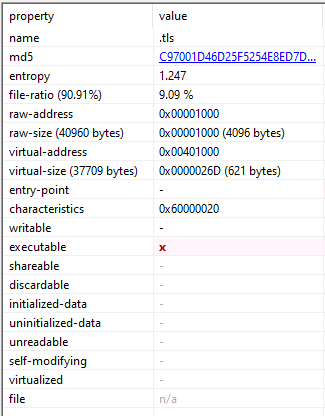
\includegraphics[width=0.4\textwidth]{pestudio-tlssection}
\caption{Esempio di sezione di un file PE che indica la presenza di una TLS Callback all'interno dell'eseguibile, analizzata con PEStudio.}
\label{fig:pestudio-tlssection}
\end{figure}

Nell'analisi statica avanzata invece la presenza di una TLS Callback è identificabile tramite la presenza di funzioni con nomi del tipo \strings{TlsCallback\_0}

\subsection*{Ricerca di breakpoint}
La ricerca di breakpoint avviene con la ricerca di istruzioni INT. Questo perchè quando si inserisce un breakpoint su una riga, l'istruzione corrispondente viene sostituita in memoria dall'istruzione esadecimale 0xCC corrispondente a:
\begin{Verbatim}
int 3
\end{Verbatim}
In questo modo la tecnica di ricerca di breakpoint scansiona in un ciclo la memoria alla ricerca dell'istruzione con valore 0xCC. 

\section{Tecniche anti-VM e anti-sandobox}

\section{Tecniche di anti-disassemblaggio}

\section{Impacchettamento}
L'impacchettamento, o \textit{Packing}, ha l'obbiettivo di impedire l'identificazione da parte di antivirus e antimalware che utilizzano il calcolo dell'hash per riconoscere malware già incontrati, oppure rendere più difficile l'analisi del malware, sia statica che dinamica.\\

Solitamente le tecniche utilizzate per impacchettare si basano sulla compressione dei dati o sulla cifratura, il che rende tutto non analizzabile. Per fare tutto ciò si ricorre ad un programma, detto \textbf{Packer}, che si occupa di impacchettare eseguibili o DLL.\\

Il Packer genera un eseguibile che, oltre a contenere il codice impacchettato, contiene anche una routine chiamata \textit{Unpacking stub}, il cui ruolo è analogo a quello che fa il sistema operativo quando deve caricare un eseguibile. Cioè il System Loader alloca in memoria RAM un'area per l'esecuzione del processo dove copia tutte le sezioni del file eseguibile. Nello stesso modo, l'unpacking stub alloca un'area di memoria nello spazio riservato per l'esecuzione del malware impacchettato, estrae il codice impacchettato, lo spacchetta risolvendo anche i riferimenti alle librerie chiamate e lo copia nell'area di memoria allocata. L'entry point, ovvero il punto in cui inizia il codice eseguibile, in un file impacchettato si trova infatti nell'unpacking stub (figura \ref{fig:packing-unpackingstub}) e, una volta terminate le operazioni di spacchettamento, viene posizionato nella sua posizione originale, cioè dove si trova il codice.

\begin{figure}[H]
\centering
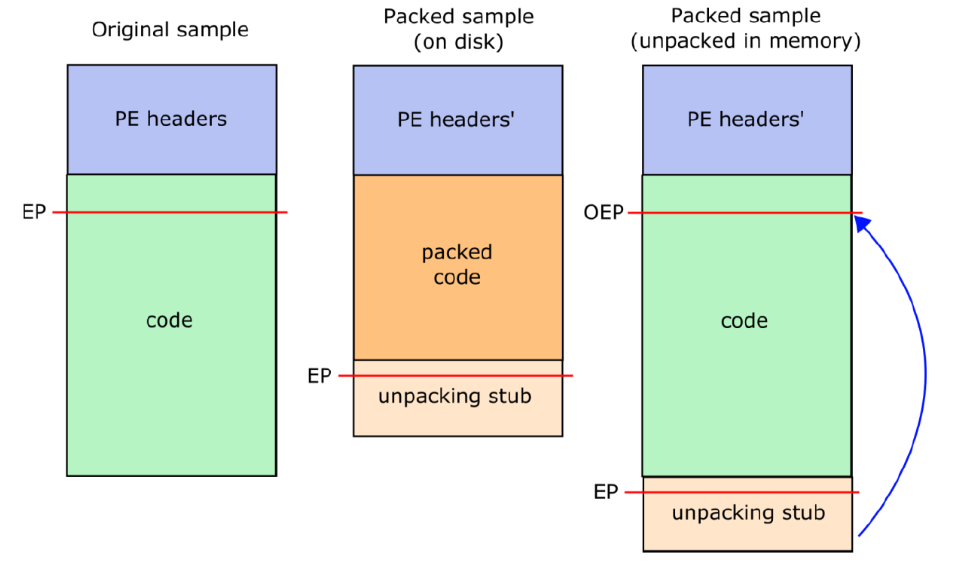
\includegraphics[width=0.75\textwidth]{packing-unpackingstub}
\caption{...}
\label{fig:packing-unpackingstub}
\end{figure}

L'unpacking si conclude quasi sempre con un'istruzione jump non condizionale (\scommand{jmp}) poichè, al termine dell'unpacking, ha bisogno di chiamare l'OEP (Original Entry Point).\\

Analizzando un malware ci si può trovare davanti diversi scenari in cui è presente un impacchettamento:
\begin{enumerate}
\item \textbf{Il Packer è ben noto}: in questo caso ci si può ritenere fortunati poichè il Packer è facilmente identificabile e le tecniche di spacchettamento si possono reperire in rete. 
\item \textbf{Il Packer è sconosciuto/personalizzato}: in questo caso chi ha scritto il malware ha creato un Packer personalizzato per il file, e lo spacchettamento deve avvenire manualmente.
\item \textbf{Il Packer è modulare}: questo è il caso peggiore in cui ci si può trovare, poichè il malware non è rappresentato da un file EXE o DLL, ma le sue funzionalità sono state suddivise in più parti di codice. Il Packer, in questo scenario, prende ciascuna di queste parti, le impacchetta e le include in un unico file eseguibile impacchettato.
\end{enumerate}

\subsection{Capire se un malware è impacchettato}
Per capire se un malware è impacchettato si può ricorrere all'analisi statica di base, in particolare PEStudio.\\
PEStudio può rivelare la signature del Packer nel campo \softwarecommand{signature} nella prima scermata una volta aperto un file PE. La signature di un packer viene ricercata in un database e non sono altro che documenti XML. Per esempio il seguente codice XML è una parte del file presente nella cartella \strings{<pestudio>\textbackslash{}xml\textbackslash{}signatures.xml} contenente le signatures riconosciute da PEStudio, in particolare è un esempio della signature di PECompact v2:
\begin{Verbatim}
<sig id="" bl="0">
  <text>PECompact v2.xx</text>
  <pattern>
    B8 xx xx xx 00 50 64 FF 35 00 00 00 00 64 89 25 00 00 00 00 33 C0
    89 08 50 45 43 6F 6D 70 61 63 74 32 00
  </pattern>
  <ep>false</ep>
</sig>
\end{Verbatim}
PEStudio non fa altro che ricercare all'interno del PE file la stringa data dal campo \scommand{<pattern>} della signature.\\

Un altro strumento molto utile è PEiD che, oltre a mostrare direttamente se il file è impacchettato oppure no, mostra dei suggerimenti su come tentare di spacchettarlo. Come fa anche PEStudio, PEiD ha un database di signature che però non è più mantenuto. In alternativa si può utilizzare ExeInfoPE e anch'esso offre un metodo suggerito per spacchettare il malware. La figura \ref{fig:exeinfope-packer} mostra un caso in cui si è trovato che il malware era impacchettato con PECompact.

\begin{figure}[H]
\centering
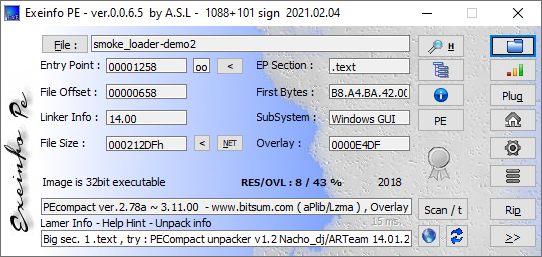
\includegraphics[width=0.75\textwidth]{exeinfope-packer}
\caption{Esempio di analisi con ExeInfoPE di un malware denominato \strings{smoke\_loader\_demo2}. Si può notare che è stato rilevato un impacchettamento con il Packer PECompact versione 2.78a, e che ExeInfoPE suggerisce di tentaro lo spacchettamento con uno strumento denominato \strings{PECompact unpacker v1.2 Nacho\_dj/ARTeam}.}
\label{fig:exeinfope-packer}
\end{figure}

\softwarename{Detect-It-Easy} è un altro software utile per l'individuazione di un packing.

Per capire se un malware è impacchettato può anche essere utile l'analisi delle stringhe: se infatti la maggior parte delle stringhe presenti sono codificate o comunque offuscate in qualche modo può essere un segnale. Gli import sono da tenere sotto controllo poichè se sono presenti librerie come stringhe ma non sono presenti nell'address table, cioè non individuabili tra gli import è un segnale che vengono caricate dinamicamente. Le funzioni presenti per un malware impacchettato sono:
\begin{itemize}
\item VirtualAlloc
\item GetProcAddress
\item LoadLibrary
\end{itemize}

Le sezioni sono un altro indicatore. Ad esempio nomi inusuali con permessi di esecuzione e scrittura, o la presenza sia della sezione .text che .CODE.

L'entropia, che misura il livello di casualità all'interno di una porzione di dati, può avere un valore che va da 0 a 8. L'implementazione comune dell'entropia è attraverso la formula di Shannon:
\[H(X) = - \sum_{i=1}^n P(x_i)\log{P(x_i)}\]
Ci dobbiamo insospettire se il valore dell'entropia di una sezione è superiore a 7.

La funzione start termina con istruzione strane!
\begin{Verbatim}
push eax
...
retn
\end{Verbatim}
C'è una possibilità che eax contenga l'Entry Point del codice originale. Bisogna utilizzare un debugger per capire quale valore viene assegnato a eax.

\begin{figure}[H]
\centering
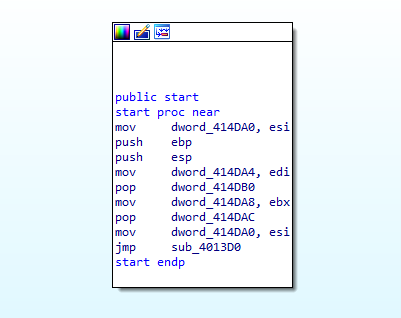
\includegraphics[width=0.5\textwidth]{ida-packedmain}
\caption{Struttura a grafo della funzione \strings{start} di un malware impacchettato, analizzato con IDA Freeware. Come si può notare è una funzione molto semplice e che possiede una JUMP non condizionale alla funzione \strings{sub\_4013D0} che molto probabilmente è la routine di spacchettamento del malware.}
\label{fig:ida-packedmain}
\end{figure}

\subsection{Come spacchettare un malware}
Ci sono diverse tecniche per fare l'unpacking di un malware.

\subsubsection*{Manualmente}
Una tecnica è quella di impostare all'interno di un debugger i breakpoint sulla funzione VirtualAlloc. Questo perchè la VirtualAlloc viene utilizzata dai malware impacchettati per allocare l'area di memoria in cui inserire il codice spacchettato. Dopodichè si esegue il malwarea fino alla chiamata di VirtualAlloc che può avvenire direttamente o indirettamente. Per controllare il valore restituito utilizzare la funzione di debug \softwarecommand{Return to User Code}. Bisogna poi ispezionare l'area di memoria appena allocato con \softwarecommand{Follow in Dump} e verificare che le chiamate successive alla VirtualAlloc vanno a modificare quell'area di memoria. Con un po' di fortuna in quell'area di memoria si trova il codice spacchettato. Considerando di utilizzare x32dbg, per impostare il breakpoint nei punti in cui viene chiamata la VirtualAlloc si può dare un comando nella sezione \softwarecommand{Command} in fondo alla finestra. Questo comando è:\\
\shellcommand{SetBPX VirtualAlloc}
e si potrà vedere nella finestra \softwarecommand{Breakpoints} il breakpoint appena impostato. Dopo che il processo si è fermato sul breakpoint di VirtualAlloc e si è cliccato \softwarecommand{Return to User code}, si può vedere che come valore di EAX c'è l'indirizzo che punta all'area di memoria appena creata, il cui contenuto è visualizzabile con \softwarecommand{Follow in Dump 1}. In questo modo in \softwarecommand{Dump 1} ci sarà sempre quell'area di memoria. Inizialmente si potrebbe trovare completamente a zero e questo significa che deve ancora essere allocata, perciò bisogna passare alla chiamata successiva e tornare successivamente a visualizzarne il contenuto. Una volta trovato l'eseguibile spacchettato cliccare su \softwarecommand{Follow in Map} e si aprirà la finestra \softwarecommand{Memory Map}. Come ultimo passaggio per salvare il file spacchettato cliccare con il tasto destro sull'indirizzo di memoria dove inizia la Dump e cliccare \softwarecommand{Dump Memory to File}.\\

Non tutte le chiamate a VirtualAlloc sono associate allo spacchettamento perciò è molto facile compiere errori. Solitamente è un processo molto lungo. Se vediamo comparire la stringa \strings{MZ} possiamo già dedurre di aver trovato il vero malware.\\

Un altro approccio invece consiste nel cercare l'OEP (Original Entry Point), ovvero il punto in cui inizia il codice eseguibile non impacchettato. Per trovarlo ci sono tre tecniche:
\begin{enumerate}
\item Section hop: il codice dell'unpacking stub e il codice del malware sono contenuti in due sezioni diverse. Di solito l'unpacking stub si trova in .text. Se inseriamo un breakpoint nel punto in cui l'esecuzione del codice passa in un'altra sezione possiamo individuare il momento in cui inzia l'esecuzione del codice spacchettato.
\item Trovare la coda del JUMP: nei casi in cui la funzione di unpacking stub termina con una JUMP non condizionale ad un indirizzo di memoria che non rientra nello stesso intervallo dell'indirzzo di memoria della funzione che si sta analizzando.
\item Push/Ret: legata all'utilizzo delle istruzioni push e ret. Casi in cui trovo una istruzione push seguita da una istruzione di return. La push potrebbe generalmente salvare l'indirizzo dell'Original Entry Point nello stack.
\end{enumerate}

\subsubsection*{\softwarename{UPX}}
Nel caso un malware sia impacchettato con UPX si può scaricare il software upx e dal terminale dare il comando:\\
\shellcommand{upx -d -o <percorso\_output> <percorso\_malware>}
dove \scommand{<percorso\_output>} corrisponde al percorso in cui volete salvare il file spacchettato, includendo anche il nome del nuovo file, mentre \scommand{<percorso\_malware>} corrisponde al percorso in cui si trova il malware da spacchettare. Nella figura \ref{fig:upx-output} è mostrato l'output risultante se l'operazione va a buon fine.

\begin{figure}[H]
\centering
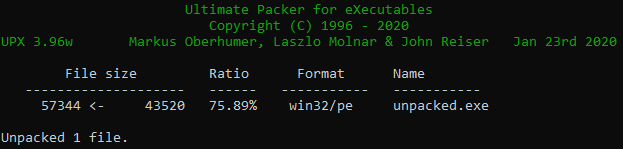
\includegraphics[width=0.7\textwidth]{upx-output}
\caption{Messaggio che viene mostrato dopo aver eseguito UPX per spacchettare un file e salvarlo in un altra cartella.}
\label{fig:upx-output}
\end{figure}

%%%%%%%%%%%%%%%%%%%%%%%%%
%% introduzione ai malware per altri sistemi
\chapter{Introduzione alla Malware Analysis per sistemi Unix}

\section{Sistemi Linux}

\section{Sistemi Mac}

%%%%%%%%%%%%%
%% esempi di analisi
\chapter {Esempi pratici di Malware Analysis}

%%%%%%%%%%%%%%%%%%%%%%%%%%%%%%%%%%%%%%%%%%%%%%%%%%%
\appendix

%%%%%%%%%%%%%
%% appendice windows
\chapter {Sistema operativo Windows}

%%
\section{Librerie ed API in Windows}
Le librerie più comunemente utilizzate in Windows sono riassunte nella seguente tabella e verranno analizzate singolarmente citando le funzioni più importati.

\section{DLL}
Una DLL è un file che contiene il riferimento alle librerie che un programma carica durante la sua esecuzione. Sono molto simili ai file .exe.

La funzione \strings{DllMain} è la funzione principale all'interno di un DLL ed è quella che verrà chiamata da un file eseguibile che vuole caricare le proprie librerie.

\subsection{Tipi di dati}
Le API di Windows lavorano con particolari tipi di dati diversi dai tipi a cui un normale programmatore potrebbe essere abituato. Sono elencati di seguito:
\begin{itemize}
\item \strings{WORD}: con prefisso \strings{w}, è un valore senza segno a 16 bit;
\item \strings{DWORD}: con prefisso \strings{dw}, è un valore senza segno a 32 bit;
\item \strings{Handle}: con prefisso \strings{H}, è un riferimento ad un oggetto;
\item \strings{Long Pointer}: con prefisso \strings{LP}, sono puntatori ad altri tipi di dati.
\end{itemize}

I prefissi sopracitati corrispondono ai valori iniziali delle variabili che contengono un particolare tipo, ad esempio un valore intero senza segno a 32 bit inizierà con \strings{dw}. Questa notazione è detta \textbf{notazione ungherese}.

I tipi \textbf{Handle} sono in pratica puntatori ad oggetti e per ottenere un handle associato ad un file basterà chiamare la funzione \strings{CreateFile} nel momento in cui si vuole crearlo e restituirà un tipo handle. Gran parte delle funzioni per modificare file e oggetti richiede come parametro un handle a tale file.

\subsection{Kernel32.dll}
\subsection{Advapi32.dll}
\subsection{User32.dll}
\subsection{Gdi32.dll}
\subsection{Ntdll.dll}
\subsection{WSock32.dll}
\subsection{Ws2\_32.dll}
\`E una libreria per gestire le connessioni in rete a basso. Ha le seguenti funzioni:
socket: crea un socket
bind: attach una socket ad una particolare porta
listen: indica che una socket è in ascolto in attesa di una connessione in entrata.
accept: apre una connessione ad un socket remoto e accetta la connessione.
connect: apre una connessione ad una socket remota che deve attendere per la connessione
recv: riceve dati dalla socket remota
send: invia dati sulla socket remota

Prima è necessario chiamare WSAStartup (?)
\subsection{Wininet.dll}
Implementa funzioni che utilizzano i protocolli di rete ad alto livello, in particolare del livello applicativo della suite di protocolli TCP/IP. Alcuni esempi sono HTTP e FTP. Le funzioni contenute in questa libreria sono:
InternetOpen: connette ad Internet
InternetOpenURL: connette ad un URL
InternetReadFile: legge il contenuto di un file scaricato dalla rete.

%%
\section{Formato Portable Executable}
Il formato PE (o Portable Executable) è un formato di file molto importante durante l'esecuzione di un file eseguibile. Il Loader, che si occupa di caricare in memoria l'eseguibile, deve caricare il codice del file, la sezione Data e importare le librerie. Per sapere tutte le informazioni per allocare lo spazio di memoria corretto e le librerie utilizzate da caricare utilizza il file PE. Il file PE contiene al suo interno informazioni come quanto spazio di memoria deve essere allocato per eseguire un file .exe, quali librerie o file DLL caricare, come sono divise le sezioni all'inteno dell'eseguibile ovvero dove finisce il codice e iniziano i dati. 

Il Loader quando alloca lo spazio di memoria da un file PE, associa un indirizzo di memoria che punta alla sezione allocata chiamato \textbf{Image Base}, inoltre il file PE ha un relative virtual address, che parte dalla prima sezione di memoria del PE e non è quindi assoluto. Per recuperare una certa allocazione nello spazio dedicato al file PE bisognerà calcolare: $ImageBase + RelativeVirtualAddress$.

Nel PE file ci possono essere anche informazioni su come viene eseguito il file .exe, ad esempio se il programma è un programma che viene lanciato da linea di comando oppure se ha un'interfaccia grafica. Un file PE è composto da diverse sezioni o header:
\begin{itemize}
\item DOS Header
\item PE Header
\end{itemize}

\subsection{DOS Header}
La prima componente di un file in formato Portable Executable è il DOS Header.  Questo è rappresentato dalla struttura sottostante che si trova all'interno dell'header winnt.h:

... struttura DOS header

e\_lfanew è un puntatore al header successivo, ovvero il PE Header.

\subsection{PE Header}
Il PE Header è una struttura di tre elementi: una signature, il File Header e l'Optional Header. La signature è una stringa ascii dal valore "PE" per indicare che il file in questione è un file PE.

\subsection{File Header}
In questo header ci sono quattro campi che servono a dare informazioni sul file corrente. Il primo campo è Machine che indica l'architettura su cui  l'eseguibile è stato progettato per girare: se a 32 bit (014C) o a 64 bit (8664). Un altro campo è il TimeDateStamp che indica quando il file è stato compilato in seconda dal 31 dicembre 1969 alle 4 PM. Il NumberOfSections indica il numero di sezioni contenute all'interno del PE file. L'ulimo campo sono le caratteristiche: una struttura con un insieme di flag e in base a quale flag è settato capiamo che tipo di file si ha davanti.

\subsection{Optional Header}
L'Optional Header è un altra struttura che, nonostante il nome, non è opzionale ed ha all'interno molti campi.

... struttura
... descrizione di tutti i campi.

\subsection{Section Header}
.text: contiene il codice da eseguire.
.data: contiene sia variabili globali o statiche il cui valore è stato inizializzato al momento della compilazione
.bss: contiene dati non inizializzati
.idata: contiene la import address table.
edata: contiene funzioni esportate dalla libreria.
.reloc: ???
.rsrc: risorse

Per ciascuna sezione esiste un header con valore Name di un byte che ci indica il nome, VirtualAddress, PointerToRawData, VirtualSize e SizeOfRawData. Esiste anche un campo Characteristics che contiene i permessi di una sezione, ovvero di scrittura, lettura ed esecuzione. 
.text deve essere sia leggibile che eseguibile
.data deve essere sia leggibile che scrivibile.

\subsection{Risorse}
Possono essere icone, immagini o qualsiasi componente dell'interfaccia grafica di un file eseguibile.

%%
\section{Registro di sistema}
Contengono informazioni su quali programmi eseguire quando un utente si collega alla macchina o quale programma è associato ad un determinato tipo di file.

I registri nel sistema Windows sono organizzati seguendo una struttura gerarchica, simile a quella del file system. Il registro radice contiene 5 cartelle principali:
\begin{itemize}
\item \strings{HKEY\_CLASSES\_ROOT}
\item \strings{HKEY\_CURRENT\_USER}
\item \strings{HKEY\_LOCAL\_MACHINE}
\item \strings{HKEY\_USERS}
\item \strings{HKEY\_CURRENT\_CONFIG}
\end{itemize}

\subsection{HKEY\_CLASSES\_ROOT}
Contiene tutte le informazioni su quali programmi eseguire associati ad ogni estensione dei file. Per esempio ...
\subsection{HKEY\_CURRENT\_USER}
Contiene tutte le informazioni sui programmi e le impostazioni legate all'utente corrente che sta utilizzando la macchina.
\subsection{HKEY\_LOCAL\_MACHINE}
Contiene tutte le informazioni legate alla macchina.
\subsection{HKEY\_USERS}
Contiene le informazioni per ciascun utente creato sulla macchina. Ogni utente ha una stringa che li associa. ... Le informazioni in \strings{HKEY\_CURRENT\_USER} sono una copia dell'utente corrente in questo registro.
\subsection{HKEY\_CURRENT\_CONFIG}
...

%%%%%%%%%%%%%
%% appendice assembly
\chapter{Linguaggio Assembly}
In questa sezione si illustrerà in maniera sintetica il funzionamento del linguaggio Assembly per architettura x86 al fine di comprendere il processo di disassemblaggio del codice malevolo che si vuole analizzare.

Il linguaggio Assembly è il linguaggio specifico per ogni architettura, qui di seguito si descriverà il linguaggio per architettura x86.

\section{Richiamo sull'architettura x86}
L'architettura x86, ma un po' tutte le architetture, ha tre componenti fondamentali: la \textit{RAM}, la \textit{CPU} e i \textit{dispositivi di Input/Output}.\\

La RAM (o Random Access Memory) è utilizzata per l'esecuzione dei programmi in quanto per ogni programma viene allocata un'area di memoria per contenerlo.\\

La CPU (o Central Processing Unit) si occupa dell'esecuzione delle istruzioni del programma. Dentro la CPU ci sono tre componenti: la Control Unit, che si occupa di recuperare le istruzioni da eseguire dallo spazio di memoria allocato per il programma, la ALU che riceve le istruzioni dal Control Unit e si occupa di decodificare le istruzioni ed eseguirle, i Registri che sono delle piccole unità di memoria utili per memorizzare i valori durante l'esecuzione delle istruzioni.\\

I dispositivi di Input/Output sono ad esempio la tastiera, il mouse, il monitor e servono a ricevere in ingresso i dati che l'utente vuole elaborare e restituirglieli.\\

..figura

\subsection*{Stuttura della memoria}
Contiene le librerie importate, lo stack, l'heap, e sezione data non allocata.

Lo stack ha una struttura a pila LIFO (Last In First Out). Gli argomenti di una funzione vengono inseriti nello stack.

\section{Endianess}
Specifica l'ordine in cui viene memorizzato un codice esadecimale associato ad una procedure. In poche parole si decide da che parte deve stare il byte meno significativo. Si può distinguere tra \textbf{Big Endian} e \textbf{Little Endian}.\\

Se si parla di \textbf{Big Endian}, un eventuale indirizzo esadecimale 0x12345678 viene salvato così com'è scritto, ovvero con il carattere più significativo a sinistra. Big Endian si utilizza all'interno dei pacchetti di rete.

Con il \textbf{Little Endian} invece, l'indirizzo utilizzato precedentemente verrà salvato come 0x78563412 (si ricorda che raggruppiamo i caratteri su 8 bit quindi si considerano coppie di caratteri esadecimali), ovvero con il byte più significativo a destra. Questa tipologia viene utlilizzata per salvare gli indirizzi in memoria RAM.

\begin{figure}[H]
\centering
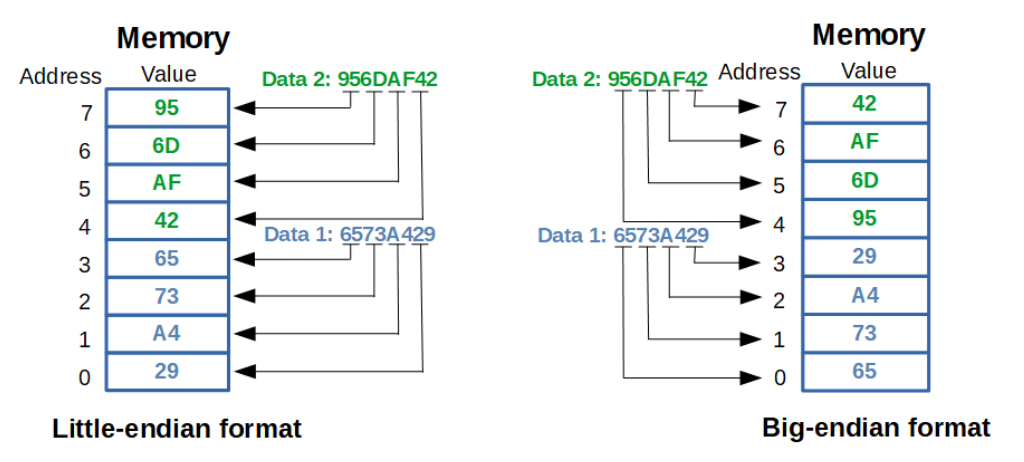
\includegraphics[width=0.8\textwidth]{endianess}
\caption{Rappresentazione del salvataggio degli indirizzi secondo le politiche di Endianess.}
\end{figure}

\section{Registri della CPU}
I registri si dividono in categorie: registri \textbf{generali}, registri di \textbf{segmento}, \textbf{flag di stato} e l'\textit{Istruction pointer}.

\subsection*{Registri generali}
Detti anche \textit{general-purpose registers}, sono registri che hanno lo scopo di memorizzare dati di operazioni aritmetiche o indirizzi di memoria. Questi registri sono 8 e possono essere immaginati come array lunghi 32 bit. Qui di seguito sono elencati i principali registri:
\begin{itemize}
\item \textbf{EAX}: registro utilizzato tipicamente per memorizzare i valori di ritorno delle funzioni;
\item \textbf{EBX}: utilizzato come \textit{base pointer} alla sezione .data;
\item \textbf{ECX}: è spesso utilizzato per implementare dei contatore per cicli come for e while;
\item \textbf{EDX}: puntatore Input/Output;
\item \textbf{ESI}: è il \textit{source pointer} per operazioni con le stringhe;
\item \textbf{EDI}: è il \textit{destination pointer} per operazioni con le stringhe;
\item \textbf{ESP}: utilizzato come \textit{stack pointer}, ovvero è un puntatore che punta sempre alla cima dello stack;
\item \textbf{EBP}: utilizzato come \textit{base pointer}, ovvero è un puntatore che punta all'inizio del frame allocato nello stack per gestire la chiamata di funzioni.
\end{itemize}

I registri EAX, EBX, ECX e EDX vengono utilizzati per salvare gli operandi durante le operazioni aritmetiche, mentre ESI e EDI sono utilizzati per operazioni con le stringhe.

\begin{figure}[H]
\centering
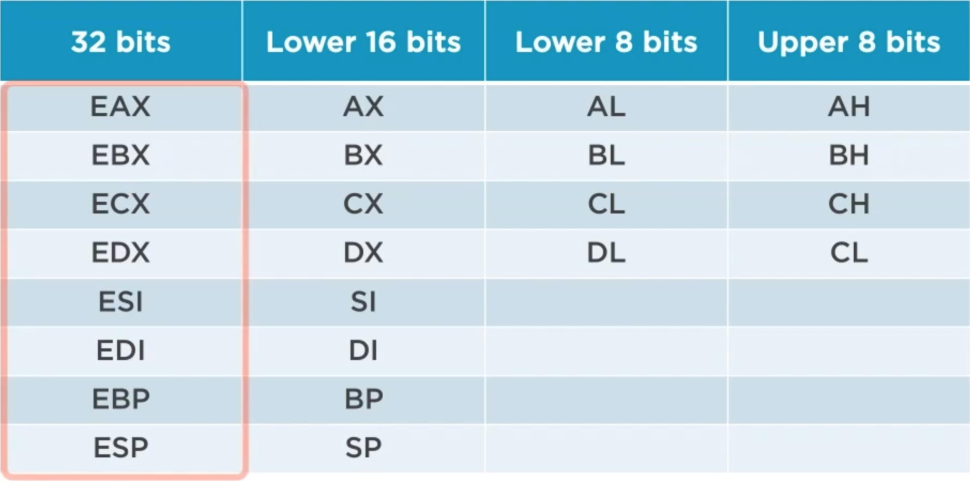
\includegraphics[width=0.8\textwidth]{general-registers}
\caption{Tabella che rappresenta i registri generali e i nomi assegnati in base ai bit presi in considerazione.}
\label{fig:general-registers}
\end{figure}

Ogni registro, come mostrato nella figura \ref{fig:general-registers}, può essere acceduto anche solo in parte: per esempio, per il registro EAX si può accedere solo ai 16 bit meno significativi e in questo caso il registro viene denominato solo AX (la E di EAX sta infatti per Extended). Il registro AX a sua volta può dare accesso solo agli 8 bit più significativi (i bit a sinistra) denominandosi AH, oppure solo agli 8 bit meno significativi (i bit a destra) denominandosi AL.

\subsection*{Registri di segmento}
Sono utilizzati per tenere traccia della posizione in memoria dello stack.

\subsection*{Flag di stato}
I flag di stato sono bit che servono a immagazzinare dei valori dovuti a risultati di operazioni aritmetiche e che possono essere utilizzati da altre istruzioni per prendere decisioni. C'è un solo registro che contiene tutti i bit di stato ed è chiamato \textbf{EFLAGS} ed è a 32 bit.\\

I bit contenuti in EFLAGS sono:
\begin{itemize}
\item \textbf{ZF}: o Zero Flag, è un bit che viene impostato a 1 quando il risultato di un'operazione è uguale a zero. Viene anche utilizzato per formulare istruzioni condizionali (equivalenti a if).
\item \textbf{CF}: o Carry Flag, è un bit che viene impostato a 1 quando il risultato di un'operazione è troppo grande o troppo piccola per essere memorizzata nel registro di destinazione.
\item \textbf{SF}: o Sign Flag, è un bit che viene impostato a 1 se il risultato di un'operazione è un numero negativo.
\item \textbf{TF}: o Trap Flag, è un bit che viene impostato a 1 nei momenti in cui si eseguono operazioni di debug.
\item ....
\end{itemize}

..tabella che mostra la distribuzione dei bit in EFLAG

\subsection*{Istruction pointer}
\`E un singolo registro che viene utilizzato per tenere traccia in memoria dell'indirizzo della prossima istruzione da eseguire.


\section{Istruzioni}
Le istruzioni in linguaggio Assembly hanno la seguente forma: il nome mnemonico dell'operazione da eseguire seguito dagli operandi, ad esempio:\\
\shellcommand{mov ecx 0x42}
Gli \textbf{operandi} possono essere di tre tipi diversi:
\begin{itemize}
\item Valore immediato, ovvero una costante come 0x42;
\item Il nome di un registro dove è presente un valore, come eax, ebx o ecx;
\item Un valore presente ad una determinata locazione di memoria, per farlo si usa la notazione \scommand{[eax]} che significa il valore contenuto nell'area di memoria rappresentata da eax. 
\end{itemize}

Qui di seguito è fornito un elenco delle istruzioni più utilizzato nel linguaggio Assembly.
\subsection*{MOV}
L'istruzione \scommand{MOV}, il cui nome deriva da move, è un istruzione utilizzata per spostare valori da un registro ad un altro, oppure per copiare un valore in un registro. La sintassi di \scommand{MOV} è:\\
\shellcommand{mov op2 op1} dove \scommand{op1} è un registro o un valore che viene copiato nel registro \scommand{op2}.

.. tabella esempi di mov

\subsection*{LEA}
L'istruzione \scommand{LEA}, acronimo di Load Effective Address, è un'istruzione simile a MOV ma con la differenza che in un registro viene copiato l'indirizzo di memoria di una allocazione e non il valore che si trova all'interno. La forma è:\\
\shellcommand{lea reg1, [mem\_addr]} dove \scommand{mem\_addr} è un indirizzo di memoria che verrà copiato nel registro \scommand{reg1}.

\subsection*{ADD}
\`E un istruzione per effettuare l'addizione. Ha la forma:\\
\shellcommand{add <dest> <src>} dove \scommand{<src>} è la sorgente dove andare a prendere il primo operando, che può essere un registro, un allocazione di memoria o un valore immediato, e \scommand{<src>}. Il risultato dell'addizione viene salvato nel registro di destinazione.
\subsection*{SUB}
Analogamente all'addizione, l'istruzione SUB compie la sottrazione tra il valore dell'operando sorgente e l'operando destinazione. Il risultato viene salvato nel registro di destinazione. Ha la forma:\\
\shellcommand{sub <dest> <src>}
Se il risultato è zero viene impostato a 1 lo Zero Flag. 
\subsection*{MUL}
L'istruzione mul effettua la moltiplicazione e, a differenza di addizione e sottrazione, ha un unico operando. La forma è quindi:\\
\shellcommand{mul <op>} con \scommand{<op>} un operando. La particolarità di questa istruzione è che utilizza un argomento implicito basato sulla grandezza dell'operando esplicito \scommand{<op>} come secondo fattore della moltiplicazione. Se l'operando esplicito ha una grandezza di a 8 bit, quello implicito andrà a leggere il valore dentro un registro di uguale grandezza (ad esempio AL) e salverà il risultato in AX. Se invece l'operando esplicito è una parola di 16 bit si andrà a leggere come secondo fattore AX e si salverà il risultato in DX e AX. La tabella mostra un esempio del funzionamento.

..tabella

\subsection*{DIV}
L'istruzione div serve per effettuare la divisione ed ha lo stesso funzionamento dell'istruzione mul. Ha la forma:
\shellcommand{div <op>} con \scommand{<op>} operando esplicito.
Il quozionte della divisione viene salvato in AL, AX o EAX, mentre il resto in AH, DX o EDX. La tabella mostra il funzionamento della divisione.

..tabella

\subsection*{AND}
Effettua l'operazione di and e segue la tabella di verita ... Ha la forma:\\
\shellcommand{and <dest> <src>} con \scommand{<dest>} operando di destinazione e \scommand{<src>} operando sorgente. L'operando di destinazione può essere solo un area di memoria o un registro, mentre l'operando sorgente può essere anche un valore immediato. 
\subsection*{OR}
Stesso funzionamento di and\\
\shellcommand{or <dest> <src>}
\subsection*{XOR}
\`E un istruzione che effettua lo XOR logico ed ha la forma:\\
\shellcommand{xor <dest> <src>} e viene spesso utilizzato per impostare a zero i valori di un registo.
\subsection*{NOT}
Ha solo un operando.
\subsection*{SHL}
SHL, che significa Shift Logical Left, è un'istruzione che effettua lo spostamento di un certo numero di bit verso sinistra. Ha due operandi e si può scrivere nella forma:\\
\shellcommand{shl <op> <shift>} dove \scommand{<op>} può essere un registro o un area di memoria ed è il valore su cui verrà effettuato lo spostamento e salvato nello stesso registro o memoria, mentre \scommand{<shift>} può essere un registro di un byte o un valore immediato (sempre di 1 byte).
\subsection*{SHR}
SHR, che significa Shift Logical Right, è un'istruzione che effettua, come lo fa la SHL, lo spostamento di un certo numero di bit però verso destra. Ha due operandi e si può scrivere nella forma:\\
\shellcommand{shr <op> <shift>} dove \scommand{<op>} può essere un registro o un area di memoria ed è il valore su cui verrà effettuato lo spostamento e salvato nello stesso registro o memoria, mentre \scommand{<shift>} può essere un registro di un byte o un valore immediato (sempre di 1 byte).
\subsection*{NOP}
NOP è un'istruzione che non fa nulla. In esadecimale ha valore 0x90.

\subsection{Istruzioni condizionali o roba simile}
\subsection*{JMP}
\`E un'Istruzione del controllo del flusso non condizionale, ovvero non verifica nessuna condizione prima di essere eseguita e salta all'istruzione dell'operando
\subsection*{JZ e JE}
Sono istruzioni di controllo del flusso condizionali ed entrambe vengono eseguite se il bit di EFLAG Zero Flag (ZF) è uguale a 1. In quel caso saltano all'istruzione passata come operando.
\subsection*{JNZ e JNE}
Sono istruzioni di controllo del flusso condizionali ed entrambe vengono eseguite se il ZF = 0
\subsection*{JL e JNGE}
Se SF = 1
\subsection*{JLE e JNG}
Se ZF = 1 o SF = 1
\subsection*{JGE e JNL}
Se SF = 0
\subsection*{CMP}
\`E un'istruzione che compara due operandi e imposta i valori dei bit di flag nel registro EFLAG in base al risultato in modo tale che possano essere acceduti da un istruzione di jump. Ha forma:\\
\shellcommand{cmp <dest> <src>} dove \scommand{<dest>} è l'operando di destinazione, mentre \scommand{<src>} è l'operando sorgente. In pratica viene sottratto l'operando sorgente all'operando destinazione e impostati i bit di flag, ma si distingue comunque dall'isturzione sub per il fatto che non salva il risultato dell'operazione nel operando \scommand{<dest>}. Modifica i bit CF, OF, SF, ZF, AF e PF. La tabella mostra un esempio di settaggi dei flag.

...tabella

\subsection*{TEST}
TEST è un'istruzione che, come cmp, effettua una comparazione dei suoi due operandi ma al contrario di cmp non effettua la sottrazione ma calcola l'AND logico e in base al risultato va a cambiare i bit di flag.

\subsection{Gestione dello stack}
\subsubsection*{PUSH}
Con l'istruzione push si va ad aggiungere un valore in cima allo stack della memoria. L'istruzione ha la forma:\\
\shellcommand{push <source>} dove la sorgente \scommand{<source>} è il valore, immediato o di un registro, che sarà inserito nello stack. L'istruzione push, una volta eseguita, decrementa automaticamente lo Stack Pointer (ESP) di 4, per allinearlo al nuovo valore.
\subsubsection*{POP}
\`E l'operazione opposta alla push e va infatti a estrarre il valore che si trova in cima allo stack e lo ritorna come DWORD mettendolo in un registro e incrementando lo Stack Pointer ESP di 4.
\subsubsection*{CALL}
L'istruzione call effettua una chiamata alla procedura rappresentata dal nome che viene passato.
\subsubsection*{RET}
Istruzione di ritorno da una procedura.... 

\section{Codice C vs. codice Assembly}
\subsection{Call Convention: stdcall}
La convenzione prevede che la stdcall rappresenti la funzione function(1,2,3) come\\
push 3\\
push 2\\
push 1\\
call function2
\subsection{Strutture condizionali IF e IF-ELSE}
esempio.
\subsection{Stuttura ciclica FOR}
esempio.
\subsection{Struttura ciclica WHILE}
esempio
\subsection*{\softwarename{Visual Studio}}
Visual Studio può esserci molto utile per visualizzare il codice assembly generato da uno script in linguaggio C che abbiamo scritto.\\

Per prima cosa aprire Visual Studio e creare un nuovo progetto con \softwarecommand{Create a new project} > \softwarecommand{Empty Project} e assegnargli un nome di progetto desiderato, dopodichè cliccare su \softwarecommand{Create}. Una volta apertosi il progetto vuoto dobbiamo creare un nuovo file in C dove scrivere il codice da visualizzare in Assembly; per farlo cliccare con il tasto destro sopra \softwarecommand{Source Files} nella finestra \softwarecommand{Solution Explorer}  e cliccare \softwarecommand{Add} > \softwarecommand{New Item}. Dopo aver fatto ciò si aprirà una finestra in sovraimpressione che permetterà di scegliere il tipo di file da creare e il nome da assegnarli: l'importante è che il file abbia estensione \softwarecommand{.c}. Cliccare su \softwarecommand{Add} per aggiungere il file al progetto, ora dovrebbe essere visualizzabile sotto \softwarecommand{Source Files}.

\subsubsection*{Impostazioni del compilatore}
Questa parte è fondamentale per far sapere al compilatore C di Visual Studio che deve evitare di eseguire alcune operazioni mentre compila. Le operazioni in questione riguardano ottimizzazioni del codice che potrebbere mostrare, una volta che abbiamo ottenuto il codice Assembly, delle istruzioni aggiuntive o addirittura togliere delle istruzioni scritte dal programmatore perchè considerate inutili. Altri esempi sono tecniche di modifica del codice utilizzate per prevenire il buffer overflow.\\

Per iniziare, cliccare con il tasto destro sul nome del proprio progetto nella finestra \softwarecommand{Solution Explorer} e selezionare \softwarecommand{Properties}. Si aprirà una finestra con un menù laterale e per ogni voce del menu una lista di opzioni. Cambiare le seguenti impostazioni come descritto qui di seguito:
\begin{itemize}
\item Su \softwarecommand{C/C++} > \softwarecommand{General} impostare:
	\begin{itemize}
	\item \textit{Debug Information Format} con il valore: \textbf{Program Database (/Zi)}
	\item \textit{Support Just My Code Debugging} con il valore: \textbf{No}
	\end{itemize}
\item Su \softwarecommand{C/C++} > \softwarecommand{Code Generation} impostare:
	\begin{itemize}
	\item \textit{Basic Runtime Checks} con il valore: \textbf{Default}
	\item \textit{Enable C++ Exceptions} con il valore: \textbf{No}
	\item \textit{Security Check} con il valore: \textbf{Disable Security Check (/GS-)}
	\end{itemize}
\item Su \softwarecommand{C/C++} > \softwarecommand{Advanced} impostare:
	\begin{itemize}
	\item \textit{Compile As} con il valore: \textbf{Compile as C Code (/TC)}
	\end{itemize}
\item Su \softwarecommand{Linker} > \softwarecommand{General} impostare:
	\begin{itemize}
	\item \textit{Enable Incremental Linking} con il valore: \textbf{No (/INCREMENTAL:NO)}
	\end{itemize}
\end{itemize}
Una volta cambiate le impostazioni cliccare su \softwarecommand{Apply}.
\subsubsection*{Visualizzazione del codice Assembly}
Supponiamo di aver scritto all'interno del file c del progetto il seguente codice C:
\begin{Verbatim}
int main(void)
{
    int a = 1;
    int b = 20;
    a = a + b;
    return 0;
}
\end{Verbatim}
Per visualizzare il codice Assembly corrispondente dobbiamo prima compilare il codice C e per farlo dobbiamo selezionare \softwarecommand{Build} > \softwarecommand{Build Solution}, dopodichè inseriamo un breakpoint sulla riga 3, ovvero la prima istruzione dentro il main, per avviare un debug e analizzare il codice Assembly riga per riga. La figura \ref{fig:visualstudio-compiled} mostra la schermata del progetto con il file in linguaggio C e il breakpoint inserito.

\begin{figure}[H]
\centering
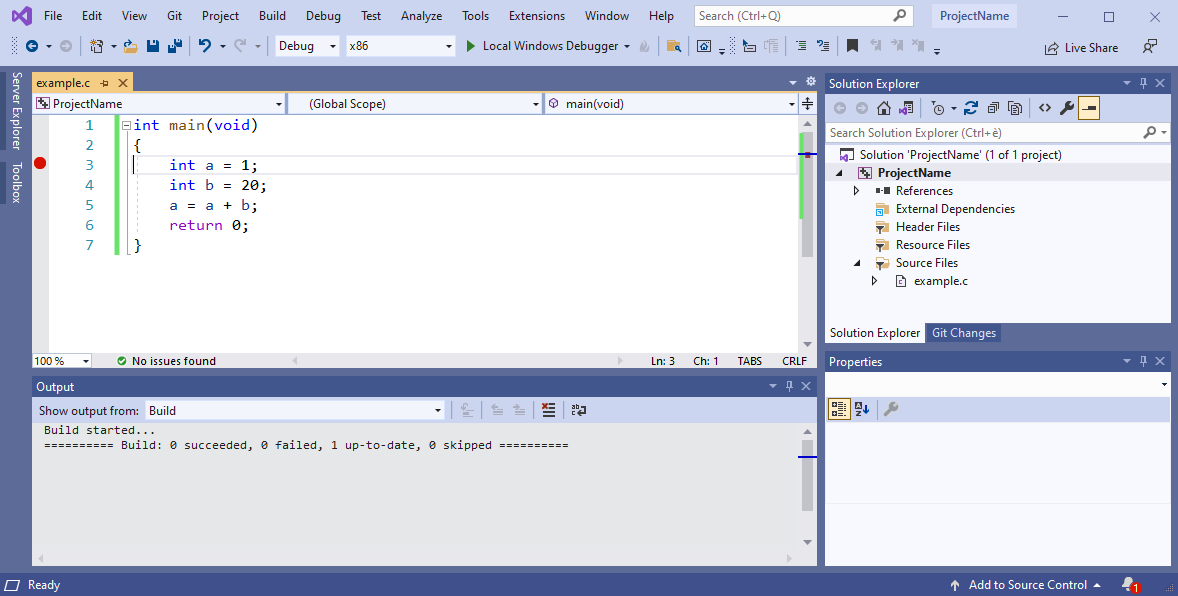
\includegraphics[width=0.98\textwidth]{visualstudio-compiled}
\caption{Schermata di VisualStudio in cui è stato creato, in un progetto, il file \strings{example.c}, contenente il codice C mostrato e compilato. \`E stato inoltre inserito un breakpoint alla riga 3.}
\label{fig:visualstudio-compiled}
\end{figure}

Per avviare il debug premere \softwarecommand{F5} oppure \softwarecommand{Debug} > \softwarecommand{Start Debugging}. Dopo aver avviato il debug è possibile passare al codice Assembly cliccando con il tasto destro nella finestra del codice e selezionando \softwarecommand{Go to Disassembly}. Fatto questo sarà possibile eseguire il debug visualizzando le istruzioni in Assembly accanto a quelle in C. La figura \ref{fig:visualstudio-assembly} mostra il codice in questione.

\begin{figure}[H]
\centering
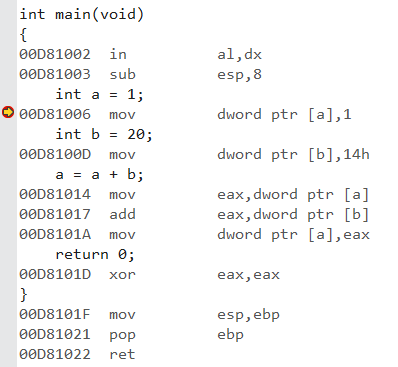
\includegraphics[width=0.5\textwidth]{visualstudio-assembly}
\caption{Codice Assembly fornito da Visual Studio durante il debug.}
\label{fig:visualstudio-assembly}
\end{figure}

In basso a sinistra nella finestra di Visual Studio comparirà una nuova finestra incorporata che mostra le schede \softwarecommand{Autos} e \softwarecommand{Locals}, le quali visualizzano rispettivamente i registri della CPU con i loro valori durante l'esecuzione e le variabili locali in C.\\

Altre due finestre molto utili che possono essere aggiunte cercandole nell'apposita barra di ricerca in alto sono: \softwarecommand{Registers} e \softwarecommand{Memory 1}. La finestra \softwarecommand{Registers} può essere cercata con \softwarecommand{Debug > Windows > Registers}  e rappresenta i valori dei registri della CPU durante l'esecuzione e viene mostrata dalla figura \ref{fig:visualstudio-registers}. 

\begin{figure}[H]
\centering
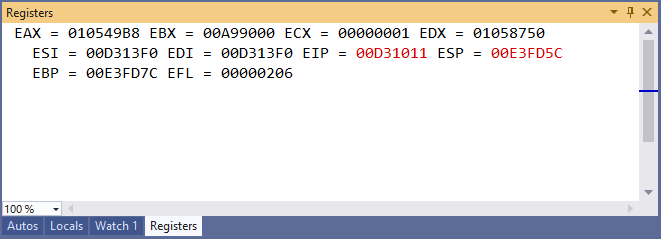
\includegraphics[width=0.8\textwidth]{visualstudio-registers}
\caption{Finestra che mostra il valore attuale dei registri della CPU, i valori in rosso sono appena stati riassegnati per esecuzione di una linea di codice all'interno del debug.}
\label{fig:visualstudio-registers}
\end{figure}

La finestra \softwarecommand{Memory 1} invece può essere cercata con  \softwarecommand{Debug > Windows > Memory 1} e mostra il contenuto della memoria durante l'esecuzione. Si possono impostare le dimensioni dei byte, la codifica e si possono cercare i registri per nome e visualizzare la riga corrispondente con il valore. La figura \ref{fig:visualstudio-memory} mostra la finestra in questione.

\begin{figure}[H]
\centering
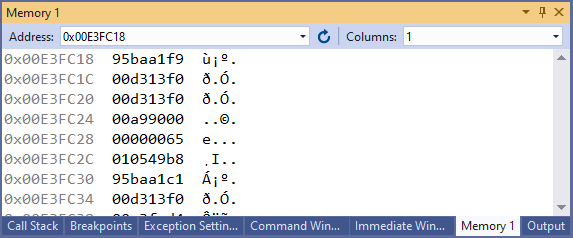
\includegraphics[width=0.8\textwidth]{visualstudio-memory}
\caption{Finestra che mostra il contenuto della memoria in byte e permette la ricerca tramite nomi dei registri.}
\label{fig:visualstudio-memory}
\end{figure}

\end{document}

